%entire chapter edited by me
%24 jan 2022
\باب{غیر تابع وقت نظریہ اضطراب}\شناخت{باب_غیر_تابع_وقت_نظریہ_اضطراب}

\حصہ{ غیر انحطاطی نظریہ اضطراب}
\جزوحصہ{ عمومی ضابطہ  بندی}
فرض کریں ہم کسی مخفیہ (مثلاً   یک  بُعدی لامتناہی چوکور کنویں) کے لئے غیر تابع وقت مساوات شروڈنگر:
\begin{align}\label{مساوات_اضطراب_پہلی}
H^0\psi_n^0=E_n^0\psi_n^0
\end{align}
حل کر کے معیاری عمودی امتیازی تفاعلات \عددی{\psi_n^0} کا مکمل سلسلہ
\begin{align}
\langle \psi_n^0 | \psi_m^0 \rangle = \delta_{nm}
\end{align}
اور ان کی مطابقتی امتیازی اقدار \عددی{E_n^0} حاصل کرتے ہیں۔ اب ہم مخفیہ میں معمولی اضطراب پیدا کرتے ہیں (مثلاً کنویں کی تہہ میں ایک چھوٹا موڑا ڈال کر؛  شکل \حوالہ{شکل_غیر_تابع_اضطراب_چکور_معمولی}) ہم  نئے  امتیازی تفاعلات اور امتیازی اقدار جاننا چاہیں گے
\begin{align}\label{مساوات_اضطراب_بنیادی}
H\psi_n = E_n\psi_n
\end{align}
%
\begin{figure}
\centering
\begin{tikzpicture}
\fill[path fading=west,color=lgray] (-0.25,0) rectangle (0,3.75);
\fill[path fading=east,color=lgray] (5,0) rectangle (5.25,3.75);
\draw[-stealth] (-0.5,0) -- (5.75,0)node[below]{$x$};
\draw[-stealth] (0,-0.25) -- (0,4)node[left]{$V(x)$};
\draw[very thick](0,3.75) -- (0,0) -- (3,0) to [out=30,in=180](3.5,0.5) to [out=0,in=150](4,0) -- (5,0)node[below]{$a$} -- (5,3.75);
\end{tikzpicture}
\caption{لامتناہی چوکور کنویں میں معمولی اضطراب}
\label{شکل_غیر_تابع_اضطراب_چکور_معمولی}
\end{figure}

تاہم ہماری  خوش قسمتی کے علاوہ ایسی   کوئی وجہ   نہیں  پائی  جاتی کہ  ہم اس  پیچیدہ مخفیہ کے لیے مساوات شروڈنگر کو بالکل ٹھیک ٹھیک حل کر  پائیں ۔ \اصطلاح{ نظریہ   اضطراب}،      غیر  مضطرب صورت کے معلوم ٹھیک ٹھیک حلوں کو لے کر،  قدم بقدم چلتے ہوئے مضطرب مسئلے کے  \ترچھا{تخمینی}  حل دیتا ہے۔  ہم نئے  ہیملٹنی کو دو اجزاء کا  مجموعہ:
\begin{align}
H = H^0 + \lambda H'
\end{align}
 لکھ کر آغاز کرتے ہیں ، جہاں \عددی{H'} اضطراب ہے (زیر بالا میں \عددی{0} ہمیشہ  غیر  مضطرب مقدار کو ظاہر کرتا ہے)۔  ہم وقتی طور پر \عددی{\lambda} کو ایک چھوٹا عدد تصور کرتے ہیں؛  بعد میں اس کی قیمت کو بڑھا کر ایک \عددی{(1)} کر دی جائے گی،  اور \عددی{H} اصل ہیملٹنی ہو گی۔ اگلے  قدم میں،   ہم \عددی{\psi_n} اور \عددی{E_n} کو \عددی{\lambda} کی طاقتی تسلسل کے صورت میں لکھتے ہیں ۔
\begin{align}
\psi_n &= \psi_n^0 + \lambda\psi_n^1 + \lambda^2\psi_n^2+\cdots \label{مساوات_اضطراب_سائے_این}\\
E_n &= E_n^0 + \lambda E_n^1 + \lambda^2 E_n^2+\cdots \label{مساوات_اضطراب_ای_این}
\end{align} 
یہاں \عددی{n} ویں امتیازی قدر کی قیمت میں \اصطلاح{اول رتبی تصحیح} کو \عددی{E_n^1} ظاہر کرتا ہے جبکہ \عددی{n} ویں امتیازی تفاعل میں \اصطلاح{اول رتبی تصحیح} کو  \عددی{\psi_n^1} ظاہر کرتا ہے؛ اسی طرح \عددی{E_n^2} اور \عددی{\psi_n^2} دوم رتبی تصحیح ہوں گی ،و غیر ه۔ مساوات \حوالہ{مساوات_اضطراب_سائے_این} اور مساوات \حوالہ{مساوات_اضطراب_ای_این} کو مساوات \حوالہ{مساوات_اضطراب_بنیادی} میں پُر کر کے 
\begin{multline*}
(H^0 + \lambda H')[\psi_n^0 + \lambda \psi_n^1 + \lambda^2 \psi_n^2 + \cdots]\\
= (E_n^0 + \lambda E_n^1 + \lambda^2 E_n^2 + \cdots)[\psi_n^0 + \lambda \psi_n^1 + \lambda^2 \psi_n^2 + \cdots]
\end{multline*}
یا ( \عددی{\lambda} کے ایک جیسے طاقتوں کو اکٹھا لکھ کر)  درج ذیل لکھا جا سکتا ہے ۔
\begin{multline*}
H^0 \psi_n^0 + \lambda (H^0 \psi_n^1 + H' \psi_n^0) + \lambda^2 (H^0 \psi_n^2 + H' \psi_n^1) + \cdots \\
= E_n^0 \psi_n^0 + \lambda (E_n^0 \psi_n^1 + E_n^1 \psi_n^0) + \lambda^2 (E_n^0 \psi_n^2 + E_n^1 \psi_n^1 + E_n^2 \psi_n^0) + \cdots
\end{multline*}
 کمتر رتبہ \عددی{(\lambda^0)} کی صورت میں\حاشیہد{ہمیشہ کی طرح، طاقتی تسلسل پھیلاو کی یکتائی  ضمانت دیتی ہے کہ  ایک جیسی طاقت کے عددی سر ایک جتنے  ہوں گے۔} اس سے \عددی{H^0 \psi_n^0 = E_n^0 \psi_n^0} حاصل ہوتا ہے،  جو   نئی مساوات نہیں ہے (مساوات \حوالہ{مساوات_اضطراب_پہلی})۔ رتبہ اول \عددی{(\lambda^1)} تک درج ذیل ہو گا ۔
\begin{align}\label{مساوات_اضطراب_رتبہ_اول}
H^0 \psi_n^1 + H' \psi_n^0 = E_n^0 \psi_n^1 + E_n^1 \psi_n^0
\end{align}
رتبہ دوم \عددی{(\lambda^2)} تک درج ذیل ہو گا 
\begin{align}\label{مساوات_اضطراب_رتبہ_دوم}
H^0 \psi_n^2 + H' \psi_n^1 = E_n^0 \psi_n^2 + E_n^1 \psi_n^1 + E_n^2 \psi_n^0
\end{align}
و غیر ه ۔ (رتبہ  پر نظر رکھنے کی غرض سے ہم نے \عددی{\lambda} استعمال کیا؛ اب اس کی کوئی  ضرورت نہیں  لہٰذا اس کی قیمت ایک، \عددی{1}، کر دیں۔)

\جزوحصہ{اول رتبی نظریہ}\شناخت{حصہ_غیر_مضطرب_اول_رتبی_نظریہ}
مساوات \حوالہ{مساوات_اضطراب_رتبہ_اول} کا \عددی{\psi_n^0} کے ساتھ اندرونی ضرب لیتے ہیں  (یعنی \عددی{(\psi_n^0)^*} سے ضرب دے کر تکمل لیتے ہیں)۔ 
\begin{align*}
\langle \psi_n^0 | H^0 \psi_n^1 \rangle + \langle \psi_n^0 | H' \psi_n^0 \rangle = E_n^0 \langle \psi_n^0 | \psi_n^0 | \psi_n^1 \rangle + E_n^1 \langle \psi_n^0 | \psi_n^0 \rangle
\end{align*}
تاہم \عددی{H^0} ہرمشی ہے لہٰذا
\begin{align*}
\langle \psi_n^0 | H^0 \psi_n^1 \rangle = \langle H^0 \psi_n^0 | \psi_n^1 \rangle = E_n^0 \langle \psi_n^0 | \psi_n^1 \rangle
\end{align*}
 ہو گا،  جو دائیں ہاتھ کے پہلے  جزو کو حدف کرے گا۔مزید  \عددی{
\langle \psi_n^0 | \psi_n^0 \rangle = 1
} 
کی بنا پر درج ذیل ہو گا ۔\حاشیہد{موجودہ سیاق و سباق میں \عددی{\langle\psi_n^0|H'\psi_n^0\rangle} یا   \عددی{\langle\psi_n^0|H'|\psi_n^0\rangle} (جہاں اضافی انتصابی  لکیر شامل کی گئی ہے)  لکھنے میں کوئی فرق نہیں، چونکہ ہم حال کو تفاعل موج کے لحاظ سے "نام"  دیتے ہیں۔لیکن موخر الذکر علامتی اظہار زیادہ بہتر ہے، چونکہ یہ ہمیں اس روایت سے آزاد کرتا ہے۔}
\begin{align}\label{مساوات_غیر_اضطراب_اہم_ترین}
E_n^1 = \langle \psi_n^0 | H' | \psi_n^0 \rangle
\end{align}
یہ رتبہ اول نظریہ اضطراب کا بنیادی نتیجہ ہے؛  بلکہ عملاً یہ پوری کوانٹائی  میکانیات میں غالباً سب سے اہم مساوات ہے۔ یہ کہتی ہے کے  غیر  مضطرب حال میں اضطراب کی توقعاتی قیمت،  توانائی کی  اول رتبی   تصحیح ہو گی۔ 

\ابتدا{مثال}\شناخت{مثال_غیر_تابع_اضطراب_چوکور_کے_تفاعلات}
لامتناہی چوکور کنویں کے غیر مضطرب تفاعلات موج (مساوات \حوالہ{مساوات_شروڈنگر_میری_سائے})   درج ذیل ہیں  ۔
\begin{align*}
\psi_n^0 (x) = \sqrt{\frac{2}{a}} \sin \big (\frac{n \pi}{a} x\big )
\end{align*}
 فرض کریں ہم کنویں کی "تہہ" (زمین)  کو مستقل مقدار \عددی{V_0} اوپر اٹھاتے ہوئے اس نظام کو مضطرب کرتے ہیں (شکل  \حوالہ{شکل_غیر_تابع_اضطراب_چکور_مستقل_اضطراب})۔   توانائیوں میں رتبہ اول  تصحیح تلاش کریں ۔

\begin{figure}
\centering
\begin{tikzpicture}
\fill[path fading=west,color=lgray] (-0.25,0) rectangle (0,3.75);
\fill[path fading=east,color=lgray] (5,0) node[below,black]{$a$} rectangle (5.25,3.75);
\draw[-stealth] (-0.5,0) -- (5.75,0)node[below]{$x$};
\draw[-stealth] (0,-0.25) -- (0,4)node[left]{$V(x)$};
\draw[very thick](0,3.75) -- (0,0.5)node[left]{$V_0$} -- (5,0.5) -- (5,3.75);
\end{tikzpicture}
\caption{پورے کنویں میں مستقل اضطراب}
\label{شکل_غیر_تابع_اضطراب_چکور_مستقل_اضطراب}
\end{figure}

حل: یہاں \عددی{H' = V_0}   ہو گا لہٰذا   \عددی{n} ویں حال کی توانائی میں رتبہ اول تصحیح درج ذیل ہو گی۔
\begin{align*}
E_n^1 = \langle \psi_n^0 | V_0 | \psi_n^0 \rangle = V_0 \langle \psi_n^0 | \psi_n^0 \rangle = V_0
\end{align*}
یوں  تصحیح  شدہ توانائیوں کی سطحیں  \عددی{E_n \cong  E_n^0 + V_0} ہوں گی؛ جی ہاں،  تمام  \عددی{V_0} مقدار  اوپر  اٹھتی ہیں۔ یہاں حیرانگی کی بات صرف  یہ ہے کہ رتبہ اول نظریہ بالکل ٹھیک جواب دیتا ہے۔ یوں ظاہر ہے کہ مستقل اضطراب کی صورت میں تمام بلند رتبی تصحیح صفر ہوں گی۔ \حاشیہد{یہاں  کوئی ی چیز لامتناہی چوکور کنویں کی خصوصیات پر منحصر نہیں ہے،  لہٰذا یہی کچھ کسی بھی مخفیہ کے لیے مستقل اضطراب کی صورت میں درست ہو گا۔} اس کے برعکس کنویں کی نصف چوڑائی تک اضطراب کی وسعت کی صورت  (شکل \حوالہ{شکل_غیر_تابع_اضطراب_نصف_چکور_مستقل_اضطراب})  میں درج ذیل   ہو گا۔
\begin{align*}
E_n^1 = \frac{2V_0}{a} \int_0^{a/2} \sin^2 \big(\frac{n \pi}{a} x\big ) \dif  x= \frac{V_0}{2}
\end{align*}
%
\begin{figure}
\centering
\begin{tikzpicture}
\fill[path fading=west,color=lgray] (-0.25,0) rectangle (0,3.75);
\fill[path fading=east,color=lgray] (5,0) rectangle (5.25,3.75);
\draw[-stealth] (-0.5,0) -- (5.75,0)node[below]{$x$};
\draw[-stealth] (0,-0.25) -- (0,4)node[left]{$V(x)$};
\draw[very thick](0,3.75) -- (0,0.5)node[left]{$V_0$} -- (2.5,0.5) -- (2.5,0)node[below]{$\tfrac{a}{2}$} -- (5,0)node[below,black]{$a$} -- (5,3.75);
\end{tikzpicture}
\caption{نصف  کنویں میں مستقل اضطراب}
\label{شکل_غیر_تابع_اضطراب_نصف_چکور_مستقل_اضطراب}
\end{figure}


اب توانائی کی ہر سطح  \عددی{\frac{V_0}{2}}اوپر  اٹھتی ہے۔ یہ غالباً بالکل ٹھیک نتیجہ نہیں،  تاہم  اول رتبی تخمین کے نقطہ نظر سے معقول جواب ہے۔
\انتہا{مثال}

 مساوات  \حوالہ{مساوات_غیر_اضطراب_اہم_ترین}  ہمیں توانائی کی اول رتبی  تصحیح دیتی ہے؛  تفاعل موج کے لئے اول رتبی تصحیح حاصل کرنے کی غرض سے ہم مساوات  \حوالہ{مساوات_اضطراب_رتبہ_اول}  کو درج ذیل روپ میں لکھتے ہے ۔
\begin{align}\label{مساوات_غیر_اضطراب_تصحیح_اول_توانائی}
(H^0 - E_n^0) \psi_n^1 = - (H' - E_n^1) \psi_n^0
\end{align}

چونکہ اس کا دایاں ہاتھ ایک معلوم تفاعل ہے،  لہٰذا یہ \عددی{\psi_n^1} کی  غیر  متجانس  تفرقی مساوات ہے۔  اب غیر مضطرب تفاعلات موج ایک مکمل سلسلہ دیتے ہیں،   لہٰذا   (کسی بھی تفاعل کی طرح)  \عددی{\psi_n^1} کو ان کا خطی جوڑ:
\begin{align}\label{مساوات_غیر_اضطراب_تصحیح_اول_تفاعل}
\psi_n^1 = \sum_{m \ne n} c_m^{(n)} \psi_m^0
\end{align}
 لکھا جا سکتا ہے ۔ اگر \عددی{\psi_n^1} مساوات \حوالہ{مساوات_غیر_اضطراب_تصحیح_اول_توانائی} کو مطمئن کرتے  ہوں تب کسی بھی مستقل \عددی{\alpha} کے لیے \عددی{(\psi_n^1 + \alpha \psi_n^0)} بھی اس مساوات کو مطمئن کریں  گے،   لہٰذا  ہم جزو \عددی{\psi_n^0} کو منفی کر سکتے ہیں؛ ایسا ہی کرتے ہوئے مساوات  \حوالہ{مساوات_غیر_اضطراب_تصحیح_اول_تفاعل}  کے مجموعہ میں \عددی{m = n} شامل نہیں کیا گیا۔ عددی سر \عددی{c_m^{(n)}} تعین کر کے ہم مسئلہ حل کر سکتے ہیں۔
 
  ہم مساوات  \حوالہ{مساوات_غیر_اضطراب_تصحیح_اول_توانائی}  میں مساوات  \حوالہ{مساوات_غیر_اضطراب_تصحیح_اول_تفاعل}  پُر کرتے ہوئے، اور  یہ جانتے ہوئے کہ غیر مضطرب مساوات  شروڈنگر   (مساوات \حوالہ{مساوات_اضطراب_پہلی})  کو \عددی{\psi_m^0} مطمئن کرتے ہیں درج ذیل حاصل کرتے ہیں ۔
\begin{align*}
\sum_{m \ne n} {(E_m^0 - E_n^0) c_m^{(n)} \psi_m^0} = - {(H' - E_n^1) \psi_n^0}
\end{align*}
اس کا \عددی{\psi_l^0} کے ساتھ اندرونی ضرب لیتے ہیں ۔
\begin{align*}
\sum_{m \ne n} (E_m^0 - E_n^0) c_m^{(n)} \langle \psi_l^0 | \psi_m^0 \rangle = - \langle \psi_l^0 | H' | \psi_n^0 \rangle + E_n^1 \langle \psi_l^0 | \psi_n^0 \rangle 
\end{align*}
اگر \عددی{l = n} ہو تب بایاں ہاتھ صفر ہو گا اور ہمیں دوبارہ مساوات  \حوالہ{مساوات_غیر_اضطراب_اہم_ترین}  ملتی ہے؛  اگر \عددی{l \ne n} ہو تو 
\begin{align*}
(E_l^0 - E_n^0) c_l^{(n)} = - \langle \psi_l^0 | H' | \psi_n^0 \rangle
\end{align*}
یا 
\begin{align}\label{مساوات_غیر_اضطراب_عددی_سر_ایم}
c_m^{(n)} = \frac{\langle \psi_m^0 | H' | \psi_n^0 \rangle}{E_n^0 - E_m^0}
\end{align}
ہو گا،  لہٰذا ا درج ذیل حاصل ہو گا ۔
\begin{align}\label{مساوات_غیر_اضطراب_تفاعل_این}
\psi_n^1 = \sum_{m \ne n} \frac{\langle \psi_m^0 | H' | \psi_n^0 \rangle}{(E_n^0 - E_m^0)} \psi_m^0
\end{align}
جب تک غیر مضطرب توانائی طیف غیر انحطاطی ہو،   نسب نما  کوئی  مسئلہ کھڑا نہیں کرتا   (چونکہ کسی بھی عددی سر کے لئے  \عددی{m = n} نہیں ہو گا)۔  ہاں  اگر  دو غیر مضطرب حالات کی توانائیاں ایک  جتنی ہوں   ( مساوات  \حوالہ{مساوات_غیر_اضطراب_عددی_سر_ایم}  کے  نسب نما میں صفر پایا جائے گا)  تب نسب نما  ہمیں مصیبت میں ڈالتا ہے؛  ایسی صورت میں \اصطلاح{ انحطاطی نظریہ اضطراب}\فرہنگ{نظریہ اضطراب!انحطاطی}\حاشیہب{degenerate perturbation theory}\فرہنگ{perturbation theory!degenerate} کی ضرورت پیش آئے گی، جس پر حصہ \حوالہ{حصہ_غیر_اضطراب_انحطاطی_نظریہ_اضطراب} میں غور کیا جائے گا۔ 

 یوں اول رتبی  نظریہ اضطراب مکمل ہوتا ہے۔  توانائی کی اول رتبی تصحیح،  \عددی{E_n^1}،  مساوات  \حوالہ{مساوات_غیر_اضطراب_اہم_ترین}  دیتی ہے،  اور  تفاعل موج کی اول رتبی  تصحیح،  \عددی{\psi_n^1}،  مساوات \حوالہ{مساوات_غیر_اضطراب_تفاعل_این} دیتی ہے۔ میں آپ کو یہاں یہ ضرور بتانا چاہوں گا کہ اگرچہ نظریہ اضطراب عموماً  توانائیوں کی انتہائی  درست قیمتیں دیتا ہے  (یعنی \عددی{E_n^0 + E_n^1}  اصل قیمت \عددی{E_n} کے بہت قریب ہو گی)،  اس سے حاصل تفاعلات موج عموماً   افسوس  کن  ہوتے ہیں۔  

\ابتدا{سوال} \شناخت{سوال_غیر_اضطراب_لامتناہی_موڑا_الف}
فرض کرے ہم لامتناہی چوکور کنویں کے وسط میں \عددی{\delta} تفاعلی موڑا:
\begin{align*}
H' = \alpha \delta \big(x - \frac{a}{2}\big)
\end{align*}
 ڈالتے ہیں ، جہاں \عددی{\alpha} ایک مستقل ہے۔ 
\begin{enumerate}[a.]
\item
 اجازتی توانائیوں کی اول رتبی تصحیح تلاش کریں۔ بتائیں   جفت \عددی{n} کی صورت میں توانائیاں کیوں  مضطرب  نہیں   ۔
\item
 زمینی حال کی  تصحیح، \عددی{\psi_1^1}،  کی اتساع    (مساوات \حوالہ{مساوات_غیر_اضطراب_تفاعل_این})   کے    ابتدائی تین غیر صفر اجزاء تلاش کریں  ۔
 \end{enumerate}
\انتہا{سوال}
\ابتدا{سوال}\شناخت{سوال_غیر_مضطرب_اجازتی_توانائیاں}
ہارمونی مرتعش \عددی{[V(x) = \tfrac{1}{2} kx^2]}  کی اجازتی توانائیاں درج ذیل ہیں 
\begin{align*}
E_n &= \big(n + \frac{1}{2}\big) \hslash \omega  && (n = 0, 1, 2, \cdots )
\end{align*}
جہاں \عددی{\omega = \sqrt{k/m}} کلاسیکی تعدد ہے۔  اب فرض کریں  مقیاس لچک میں معمولی تبدیلی رونما ہوتی ہے: \عددی{k \to (1 + \epsilon ) k}، (جس سے اسپرنگ کی لچک کم ہو گی)۔
\begin{enumerate}[a.]
\item
 نئی  توانائیوں کی بالکل ٹھیک ٹھیک قیمتیں  حاصل  کریں  (جو یہاں ایک آسان کام ہے)۔ اپنے  کلیہ کو دوم رتبہ تک \عددی{\epsilon} کی طاقتیں تسلسل میں پھیلائیں۔ 
\item
 اب مساوات \حوالہ{مساوات_غیر_اضطراب_اہم_ترین}  استعمال کرتے ہوئے توانائی میں اول رتبی اضطراب کا حساب لگائیں۔ یہاں \عددی{H'} کیا  ہو گا؟  اپنے نتیجے کا جزو-ا کے ساتھ موازنہ کریں۔ \ترچھا{ اشارہ:} یہاں کسی نئے تکمل کی قیمت کے حصول کی نہ ضرورت اور نہ اجازت ہے ۔
 \end{enumerate}
\انتہا{سوال} 
\ابتدا{سوال}
ایک لامتناہی چوکور کنویں (مساوات  \حوالہ{مساوات_شروڈنگر_لامتناہی_چکور})   میں دو یکساں بوسن رکھے جاتے ہیں۔ یہ مخفیہ 
\begin{align*}
V(x_1, x_2) = -aV_0\delta (x_1 - x_2)
\end{align*}
( جہاں \عددی{V_0} ایک مستقل   جس کا بُعد توانائی ہے  اور \عددی{a} کنویں کی چوڑائی ہے)  کے ذریعے ایک دوسرے پر بہت معمولی اثر انداز ہوتے ہیں ۔
\begin{enumerate}[a.]
\item
 پہلے قدم میں،  ذرات کے باہمی   اثر  کو نظر انداز کرتے ہوئے، زمینی حال اور پہلے ہیجان حال کے تفاعلات موج اور مطابقتی توانائیاں تلاش کریں ۔
\item
 زمینی حال اور پہلے    ہیجان  حال کی  توانائیوں پر ذرات کے باہمی  اثر کا تخمین اول رتبی نظریہ اضطراب سے دریافت کریں ۔
 \end{enumerate}
\انتہا{سوال} 


%====================
\جزوحصہ{دوم رتبی توانائیاں}\شناخت{حصہ_غیر_اضطراب_دوم_رتبی_توانائیاں}
 اسی طرح بڑھتے ہوئے،  ہم \عددی{\psi_n^0} اور دو رتبی مساوات (مساوات \حوالہ{مساوات_اضطراب_رتبہ_دوم}) کا اندرونی ضرب لیتے ہیں ۔
\begin{align*}
\langle \psi_n^0 | H^0 \psi_n^2 \rangle + \langle \psi_n^0 | H' \psi_n^1 \rangle = E_n^0 \langle \psi_n^0 | \psi_n^2 \rangle + E_n^1 \langle \psi_n^0 | \psi_n^1 \rangle + E_n^2 \langle \psi_n^0 | \psi_n^0 \rangle
\end{align*}
یہاں بھی ہم \عددی{H^0} کے ہرمشی پن کو بروئے کار لاتے ہیں: 
\begin{align*}
\langle \psi_n^0 | H^0 \psi_n^2 \rangle = \langle H^0 \psi_n^0 | \psi_n^2 \rangle = E_n^0 \langle \psi_n^0 | \psi_n^2 \rangle
\end{align*}
 لہٰذا  بائیں ہاتھ کا پہلا جزو دائیں ہاتھ کے پہلے جزو کے ساتھ کٹ جائے گا۔   ساتھ   ہی \عددی{\langle \psi_n^0 | \psi_n^0 \rangle = 1} ہے    لہٰذا    \عددی{E_n^2} کا درج ذیل  کلیہ حاصل ہوتا ہے۔
\begin{align}\label{مساوات_غیر_مضطرب_دوم_رتبی_تصحیح}
E_n^2 = \langle \psi_n^0 | H' | \psi_n^1 \rangle - E_n^1 \langle \psi_n^0 | \psi_n^1 \rangle
\end{align}
تاہم  مجموعہ  میں \عددی{m = n} شامل نہیں  اور  باقی تمام عمودی ہیں  لہٰذا  
\begin{align*}
\langle \psi_n^0 | \psi_n^1 \rangle  = \sum_{m \ne n} c_m^{(n)} \langle \psi_n^0 | \psi_m^0 \rangle = 0
\end{align*}
 ہو گا جس کی بنا پر 
\begin{align*}
E_n^2 = \langle \psi_n^0 | H' | \psi_n^1 \rangle = \sum_{m \ne n} c_m^{(n)} \langle \psi_n^0 | H' | \psi_m^0 \rangle = \sum_{m \ne n} \frac{\langle \psi_m^0 | H' | \psi_n^0 \rangle \langle \psi_n^0 | H' | \psi_m^0 \rangle }{E_n^0 - E_m^0}
\end{align*}
یا  
\begin{align}\label{مساوات_غیر_اضطراب_دوم_رتبی_نتیجہ}
E_n^2 = \sum_{m \ne n} \frac{ \abs{ \langle \psi_m^0 | H' | \psi_n^0\rangle }^2 }{E_n^0 - E_m^0}
\end{align}
 ہو گا۔ یہ  دو رتبی نظریہ اضطراب کا بنیادی نتیجہ ہے۔

 اگرچہ ہم اسی طرح آگے بڑھتے ہوئے تفاعل موج   \عددی{(\psi_n^2)}   کی  دوم رتبی تصحیح،  توانائی کی سوم  رتبی تصحیح،  وغیرہ  حاصل کر سکتے ہیں،  لیکن عملاً اس ترکیب کو صرف مساوات \حوالہ{مساوات_غیر_اضطراب_دوم_رتبی_نتیجہ} تک استعمال کرنا سودمند  ہو گا۔\حاشیہد{مختصر انداز لکھائی میں
 \عددی{V_{mn}\equiv \langle \psi_m^0|H'|\psi_n^0\rangle}، \عددی{\Delta_{mn}\equiv E_m^0-E_n^0} اور \عددی{n} ویں توانائی کی پہلی تین تصحیح درج ذیل  ہوں گی۔
 \begin{align*}
 E_n^1=V_{nn},\quad E_n^2=\sum_{m\ne n} \frac{\abs{V_{nm}}^2}{\Delta_{nm}},\quad E_n^3=\sum_{l,m\ne n} \frac{V_{nl}V_{lm}V_{mn}}{\Delta_{nl}\Delta_{nm}}-V_{nn}\sum_{m\ne n}\frac{\abs{V_{nm}}^2}{\Delta_{nm}^2}
 \end{align*}
 }
 
\ابتدا{سوال}
\begin{enumerate}[a.]
\item
توانائیوں کی  دوم رتبی  تصحیح  \عددی{(E_n^2)}،  سوال  \حوالہ{سوال_غیر_اضطراب_لامتناہی_موڑا_الف}   کے  مخفیہ کے لیے تلاش کریں۔ \ترچھا{ تبصرہ:}  آپ تسلسل کا مجموعہ صریحاً حاصل کر کے طاق \عددی{n} کیلئے  \عددی{-2m( \alpha / \pi \hslash n)^2} حاصل کر سکتے ہیں۔
\item
زمینی حال توانائی کے لئے دوم رتبی تصحیح  \عددی{(E_n^2)}،  سوال  \حوالہ{سوال_غیر_مضطرب_اجازتی_توانائیاں}  کے مخفیہ کے لیے تلاش کریں۔ تصدیق کریں  کہ آپ کا نتیجہ بالکل درست نتیجے کے مطابق ہے۔ 
\end{enumerate}
\انتہا{سوال}
\ابتدا{سوال}
ایک ایسے  باردار  ذرہ پر غور کریں جو یک بُعدی ہارمونی ارتعاشی مخفیہ  میں پایا جاتا ہو۔ فرض کریں  ہم ایک کمزور برقی میدان \عددی{(E)} چالو کرتے ہیں جس کی بنا پر مخفی توانائی میں \عددی{H' = qEx} مقدار کی تبدیلی پیدا ہوتی ہے۔
\begin{enumerate}[a.]
\item
دکھائیں کہ توانائیوں کی  دو سطحوں میں کوئی اول رتبی تبدیلی پیدا نہیں ہو گی۔ دو رتبی تصحیح  تلاش کریں۔\ترچھا{ اشارہ:}  سوال  \حوالہ{سوال_قواعد_قالبی_ارکان}  دیکھیں۔
\item
تبدیلی متغیرات \عددی{x' \equiv x - (qE/m \omega^2)} استعمال کرتے ہوئے موجودہ صورت میں مساوات  شروڈنگر  کو بلا واسطہ حل کیا جا سکتا ہے۔ ایسا کرتے ہوئے ٹھیک ٹھیک توانائیاں تلاش کر کے دکھائیں کہ یہ نظریہ اضطراب کی تخمین کے مطابق ہیں۔
\end{enumerate}
\انتہا{سوال}




\حصہ{انحطاطی نظریہ اضطراب}\شناخت{حصہ_غیر_اضطراب_انحطاطی_نظریہ_اضطراب}
اگر غیر مضطرب حالات انحطاطی ہوں؛  یعنی،  دو (یا دو سے زیادہ)  منفرد حالات ( \عددی{\psi_a^0} اور \عددی{\psi_b^0})  کی توانائیاں ایک  جیسی ہوں،  تب سادہ نظریہ اضطراب غیر کارآمد ہو گا،  چونکہ \عددی{c_a^{(b)}} (مساوات  \حوالہ{مساوات_غیر_اضطراب_عددی_سر_ایم})   اور \عددی{E_a^2} (مساوات \حوالہ{مساوات_غیر_اضطراب_دوم_رتبی_نتیجہ})  بےقابو بڑھتے ہیں  ( ماسوائے اس صورت میں  جب شمار کنندہ صفر ہو:  \عددی{\langle \psi_a^0 | H' | \psi_b^0 \rangle = 0}؛  اس  پوشیدہ   صورت   کو ہم بعد میں استعمال کریں گے)۔ یوں  انحطاطی صورت میں ہمیں توانائیوں کی اول  رتبی تصحیح ( مساوات \حوالہ{مساوات_غیر_اضطراب_اہم_ترین})   پر بھی یقین نہیں کرنا چاہیے اور ہمیں مسئلے کا کوئی دوسرا حل ڈھونڈنا   ہو گا۔


\جزوحصہ{دو پڑتا انحطاط}\شناخت{حصہ_غیر_مضطرب_دو_پڑتا_انحطاط}
درج ذیل فرض کریں جہاں \عددی{\psi_a^0} اور \عددی{\psi_b^0} معمول شدہ ہیں۔
\begin{align}\label{مساوات_غیر_مضطرب_دو_پڑتا_اضطراب}
H^0 \psi_a^0 = E^0 \psi_a^0, \quad H^0 \psi_b^0 = E^0 \psi_b^0, \quad \langle \psi_a^0 | \psi_b^0 \rangle = 0
\end{align}
دھیان رہے کہ ان حالات کا ہر خطی جوڑ 
\begin{align}\label{مساوات_غیر_مضطرب_دو_پڑتا_عمومی}
\psi^0 = \alpha \psi_a^0 + \beta \psi_b^0
\end{align}
بھی \عددی{H^0} کا امتیازی حال ہو گا اور اس  کی  امتیازی قدر \عددی{E^0} بھی وہی ہو گی۔ 
\begin{align}\label{مساوات_غیر_مضطرب_دو_پڑتا_وہی_توانائی}
H^0 \psi^0 = E^0 \psi^0
\end{align}

\begin{figure}
\centering
\begin{tikzpicture}
\draw[-stealth] (0,0) -- (6,0) node[below]{$\lambda$};
\draw[-stealth] (0,0) -- (0,4) node[left]{$E$};
\draw[thick] (0,2) to [out = 0, in=-140] (5,3.75);
\draw[thick] (0,2)node[left]{$E_0$} to [out = 0, in=140] (5,0.25);
\draw[dashed] (5,0) node[below]{$1$} -- (5, 4);
\end{tikzpicture}
\caption{انحطاط کا خاتمہ بذریعہ اضطراب۔}
\label{شکل_غیر_تابع_اضطراب_اختتام_انحطاط}
\end{figure}


عام طور پر اضطراب \عددی{(H')} انحطاط کو "توڑے"  (یا "منسوخ" کرے) گا:  جیسے جیسے ہم \عددی{\lambda} کی قیمت ( \عددی{0} سے \عددی{1}  کی طرف) بڑھاتے ہیں مشترک غیر مضطرب توانائی \عددی{E^0} دو ٹکڑوں میں تقسیم ہو گی   (شکل  \حوالہ{شکل_غیر_تابع_اضطراب_اختتام_انحطاط})۔ مخالف رخ  چلتے ہوئے اگر ہم اضطراب کو بند (  یعنی صفر)  کر دیں تب "بالائی"  حال کی تخفیف ،  \عددی{\psi_a^0} اور \عددی{\psi_b^0} کے  ایک خطی جوڑ میں  جبکہ" زیریں" حال کی تخفیف کسی دوسرے  \ترچھا{عمودی} خطی جوڑ میں ہو گا،   تاہم ہم قبل از وقت نہیں جان سکتے  کہ یہ" \اصطلاح{موزوں}"\فرہنگ{موزوں!خطی جوڑ}\حاشیہب{good linear combinations}\فرہنگ{good!linear combinations} خطی جوڑ کیا ہوں گے۔ چونکہ ہم غیر مضطرب حالات نہیں جانتے،   لہٰذا    ہم اول رتبی توانائیوں  (مساوات  \حوالہ{مساوات_غیر_اضطراب_اہم_ترین}) کا حساب نہیں کر سکتے۔ 

اسی لیے، ہم ان "موزوں" غیر مضطرب حالات کو فی الحال عمومی روپ (مساوات  \حوالہ{مساوات_غیر_مضطرب_دو_پڑتا_عمومی})   میں لکھتے ہیں،  جہاں \عددی{\alpha} اور \عددی{\beta} قابل تغیر ہوں گے۔ ہم مساوات شروڈنگر
\begin{align}\label{مساوات_غیر_مضطرب_مساوات_شروڈنگر}
H \psi = E \psi
\end{align}
کو \عددی{H = H^0 + \lambda H'} اور 
\begin{align}
E = E^0 + \lambda E^1 + \lambda^2 E^2 + \cdots, \quad \psi = \psi^0 + \lambda \psi^1 + \lambda^2 \psi^2 + \cdots
\end{align}
کیلئے حل کرنا چاہتے ہیں۔  انہیں مساوات \حوالہ{مساوات_غیر_مضطرب_مساوات_شروڈنگر} میں ڈال  کر  (ہمیشہ کی طرح)  \عددی{\lambda} کی ایک جیسی طاقتیں اکٹھی کر کے درج ذیل حاصل  کرتے ہیں ۔
\begin{align*}
H^0 \psi^0 + \lambda (H' \psi^0 + H^0 \psi^1) + \cdots = E^0 \psi^0 + \lambda (E^1 \psi^0 + E^0 \psi^1) + \cdots
\end{align*}
اب \عددی{H^0 \psi^0 = E^0 \psi^0} (مساوات \حوالہ{مساوات_غیر_مضطرب_دو_پڑتا_وہی_توانائی})   کی بنا پر اولین اجزاء ایک دوسرے کے ساتھ کٹ جائیں گے،  جبکہ \عددی{\lambda^1} رتبہ کے لیے درج ذیل ہو گا ۔
\begin{align}
H^0 \psi^1 + H' \psi^0 = E^0 \psi^1 + E^1 \psi^0
\end{align}
اس کا \عددی{\psi_a^0} کے ساتھ اندرونی ضرب لیتے ہیں ۔
\begin{align*} 
\langle \psi_a^0 | H^0 \psi^1 \rangle + \langle \psi_a^0 | H' \psi^0 \rangle = E^0 \langle \psi_a^0 | \psi^1 \rangle + E^1 \langle \psi_a^0 | \psi^0 \rangle
\end{align*}
چونکہ \عددی{H^0} ہرمشی ہے،  لہٰذا  بائیں ہاتھ پہلا جزو دائیں ہاتھ کے پہلے جزو کے ساتھ کٹ جائے گا۔  مساوات \حوالہ{مساوات_غیر_مضطرب_دو_پڑتا_عمومی}  کو استعمال کرتے ہوئے اور معیاری عمودیت کی شرط (مساوات  \حوالہ{مساوات_غیر_مضطرب_دو_پڑتا_اضطراب})   کو بروئے کار لاتے ہوئے 
\begin{align*}
\alpha \langle \psi_a^0 | H' | \psi_a^0 \rangle + \beta \langle \psi_a^0 | H' | \psi_b^0 \rangle = \alpha E^1
\end{align*}
یا مختصراً
\begin{align}\label{مساوات_غیر_مضطرب_اندرونی_ضرب_اول}
\alpha W_{aa} + \beta W_{ab} = \alpha E^1
\end{align}
حاصل ہو گا جہاں درج ذیل ہو گا ۔
\begin{align}\label{مساوات_غیر_مضطرب_مختصر}
W_{ij} \equiv \langle \psi_i^0 | H' | \psi_j^0 \rangle, \quad (i, j = a, b)
\end{align}
اسی طرح \عددی{\psi_b^0} کے ساتھ اندرونی ضرب درج ذیل دے گا ۔
\begin{align}\label{مساوات_غیر_مضطرب_اندرونی_ضرب_دوم}
\alpha W_{ba} + \beta W_{bb} = \beta E^1
\end{align}

دھیان رہے کہ( اصولاً)  ہمیں تمام \عددی{W} معلوم ہیں،  چونکہ یہ غیر مضطرب تفاعلات موج \عددی{\psi_a^0} اور \عددی{\psi_b^0} کے لحاظ سے \عددی{H'} کے ارکان قالب ہیں۔  مساوات  \حوالہ{مساوات_غیر_مضطرب_اندرونی_ضرب_دوم}   کو \عددی{W_{ab}} سے ضرب دے کر،  مساوات  \حوالہ{مساوات_غیر_مضطرب_اندرونی_ضرب_اول}  استعمال کرتے ہوئے  \عددی{\beta W_{ab}} کو خارج کر کے،  درج ذیل حاصل ہو گا ۔
\begin{align}\label{مساوات_غیر_مضطرب_پہلا_اچھا_نتیجہ}
\alpha [W_{ab} W_{ba} - (E^1 - W_{aa}) (E^1 - W_{bb})] = 0
\end{align}
غیر صفر \عددی{\alpha} کی صورت میں مساوات  \حوالہ{مساوات_غیر_مضطرب_پہلا_اچھا_نتیجہ}  ہمیں \عددی{E^1} کی مساوات دیگی۔ 
\begin{align}\label{مساوات_غیر_مضطرب_امتیازی_مساوات}
(E^1)^2 - E^1 (W_{aa} + W_{bb}) + (W_{aa} + W_{bb} - W_{ab} W_{ba}) = 0
\end{align}
دو درجی کلیہ استعمال کرتے ہوئے اور( مساوات \حوالہ{مساوات_غیر_مضطرب_مختصر}  سے)  جانتے ہوئے کہ  \عددی{W_{ba} = W^*_{ab}} ہو گا،  ہم درج ذیل اخذ کرتے ہیں ۔
\begin{align}\label{مساوات_غیر_مضطرب_مضطرب_تونائیاں}
E_{\pm}^1 = \frac{1}{2} \left[W_{aa} + W_{bb} \pm \sqrt{(W_{aa} - W_{bb})^2 + 4 \abs{W_{ab}}^2} \,\,\right ]
\end{align}
یہ انحطاطی نظریہ اضطراب کا بنیادی نتیجہ ہے، جہاں دو  جذر دو مضطرب توانائیوں   ہیں۔

 لیکن صفر \عددی{\alpha} کی صورت میں کیا ہو گا؟ ایسی صورت میں \عددی{\beta = 1} ہو گا، لہٰذا     مساوات  \حوالہ{مساوات_غیر_مضطرب_اندرونی_ضرب_اول}  کے تحت \عددی{W_{ab} = 0} اور مساوات \حوالہ{مساوات_غیر_مضطرب_اندرونی_ضرب_دوم}  کے تحت \عددی{E^1 = W_{bb}} ہو گا۔ یہ درحقیقت  عمومی نتیجہ  (مساوات \حوالہ{مساوات_غیر_مضطرب_مضطرب_تونائیاں})   میں منفی علامت کے ذریعے  شامل ہے ( مثبت علامت \عددی{\alpha = 1}، \عددی{\beta = 0} کی صورت میں ہو گا)۔ اس کے علاوہ ہمارے جوابات 
\begin{align*}
E_{+}^1 = W_{aa} = \langle \psi_a^0 | H' | \psi_a^0 \rangle, \quad E_{-}^1 = W_{bb} = \langle \psi_b^0 | H' | \psi_b^0 \rangle
\end{align*}
ٹھیک وہی ہیں جو  غیر انحطاطی نظریہ اضطراب سے حاصل  ہوتے ( مساوات  \حوالہ{مساوات_غیر_اضطراب_اہم_ترین})۔   یہ محض ہماری خوش قسمتی ہے:  حالات \عددی{\psi_a^0} اور \عددی{\psi_b^0} پہلے سے "موزوں" خطی جوڑ تھے۔ کیا اچھا ہوتا،  اگر ہم آغاز سے ہی  " موزوں" حالات جان پاتے؛   تب  ہم غیر انحطاطی نظریہ اضطراب استعمال کر پاتے۔  حقیقت میں درج ذیل مسئلہ کے تحت ہم عموماً ایسا کر پاتے ہیں ۔

\ابتدا{مسئلہ}
فرض کریں \عددی{A} ایک ایسا ہرمشی عامل ہے،  جو \عددی{H^0} اور \عددی{H'} کے ساتھ  مقلوبی  ہے۔  اگر( \عددی{H^0} کے انحطاطی امتیازی تفاعلات)  \عددی{\psi_a^0} اور \عددی{\psi_b^0} عامل \عددی{A} کے بھی امتیازی تفاعلات ہوں،  جن کے منفرد امتیازی اقدار ہوں،
\begin{align*}
\text{\RL{ہو}}\quad \mu\ne \nu\quad \text{\RL{اور}}\quad A \psi_a^0 = \mu \psi_a^0, \quad A \psi_b^0 = \nu \psi_b^0 
\end{align*} 
تب \عددی{W_{ab} = 0} ہو گا ( لہٰذا  \عددی{\psi_a^0} اور \عددی{\psi_b^0} نظریہ اضطراب میں قابل استعمال،  "موزوں" حالات ہوں گے)۔
\انتہا{مسئلہ}
\ابتدا{ثبوت}
ہم فرض کر چکے  کہ \عددی{[A, H'] = 0} ہو گا لہٰذا  درج ذیل ہو گا ۔
\begin{align*}
\langle \psi_a^0 | [A, H'] \psi_b^0 \rangle &= 0 \\
&= \langle \psi_a^0 | A H' \psi_b^0 \rangle - \langle \psi_a^0 | H' A \psi_b^0 \rangle \\
&= \langle A \psi_a^0 | H' \psi_b^0 \rangle - \langle \psi_a^0 | H' \nu \psi_b^0 \rangle \\
&= (\mu - \nu) \langle \psi_a^0 | H' \psi_b^0 \rangle = (\mu - \nu) W_{ab} 
\end{align*}
اب \عددی{\mu \ne \nu} ہے لہٰذا  \عددی{W_{ab} = 0} ہو گا ۔

\موٹا{سبق:}   اگر آپ کا سامنا انحطاطی حالات سے ہو،  ایسا ہرمشی عامل \عددی{A} تلاش کرنے کی کوشش کریں جو \عددی{H^0} اور \عددی{ H'} کے ساتھ  مقلوبی  ہو؛  \عددی{ H^0} اور \عددی{ A} کے بیک وقت امتیازی تفاعلات کو  غیر مضطرب حالات منتخب کر کے سادہ اول رتبی نظریہ اضطراب بروئے کار لائیں۔ ایسے عامل کی  تلاش  میں ناکامی  کی صورت میں آپ کو مساوات \حوالہ{مساوات_غیر_مضطرب_مضطرب_تونائیاں}  استعمال کرنا ہو گا،  جس کی ضرورت عملاً  کم ہی پڑتی ہے ۔
\انتہا{ثبوت} 
%=============================
\ابتدا{سوال}
  دو"موزوں" غیر مضطرب حالات
\begin{align*}
\psi_\pm^0 = \alpha_\pm \psi_a^0 + \beta_\pm \psi_b^0
\end{align*}
لیں، جہاں \عددی{\alpha_\pm} اور \عددی{\beta_\pm} کو( معمول زنی  تک)  مساوات \حوالہ{مساوات_غیر_مضطرب_اندرونی_ضرب_اول} (  یا مساوات \حوالہ{مساوات_غیر_مضطرب_اندرونی_ضرب_دوم})   تعین کرتا ہے۔   صریحاً  درج ذیل دکھائیں ۔
\begin{enumerate}[a.]
\item
\عددی{\psi_\pm^0} عمودی ہیں:  \عددی{(\langle \psi_+^0 | \psi_-^0 \rangle = 0)}  ؛
\item
\عددی{\langle \psi_+^0 | H' | \psi_-^0 \rangle = 0} ؛
\item
\عددی{\langle\psi_\pm^0 | H' | \psi_\pm^0 \rangle = E_\pm^1} جہاں \عددی{E_{\pm}^1} کی قیمت مساوات \حوالہ{مساوات_غیر_مضطرب_مضطرب_تونائیاں} دیتی ہے۔ 
\end{enumerate}
\انتہا{سوال} 
\ابتدا{سوال} 
فرض کرے ایک ذرہ،  جس کی کمیت \عددی{m} ہے،  ایک  بند یک بُعدی تار،  جس کی لمبائی \عددی{L} ہے،  پر آزادی سے حرکت کرتا ہے (سوال \حوالہ{سوال_غیر_تابع_شروڈنگر_بے_رگڑ_موتی})۔ 
\begin{enumerate}[a.]
\item
دکھائیں کے ساکن حالات کو درج ذیل روپ میں لکھا جا سکتا ہے 
 \begin{align*}
\psi_n (x) &= \frac{1}{\sqrt{L}} e^{2 \pi i n x/ L}, &&(-L/2 < x < L/2)
\end{align*}
جہاں \عددی{ n = 0, \pm 1, \pm 2, \dotsc} اور اجازتی توانائیاں درج ذیل ہوں گی۔
\begin{align*}
E_n = \frac{2}{m} \big ( \frac{n \pi \hslash}{L} \big )^2
\end{align*}
دھیان رہے کہ زمینی حال \عددی{( n = 0)} کے علاوہ تمام حالات دہرے  انحطاطی ہیں۔ 
\item
فرض کریں ہم اب اضطراب 
\begin{align*}
H' = -V_0 e^{-x^2 / a^2}
\end{align*}
متعارف کرتے ہیں جہاں \عددی{a \ll L} ہے۔ ( یہ \عددی{ x = 0} پر مخفیہ میں ایک ٹویا  پیدا کرتا ہے، گویا    تار کو مروڑ   کر پکڑ بنایا  گیا ہو۔) مساوات \حوالہ{مساوات_غیر_مضطرب_مضطرب_تونائیاں}  استعمال کرتے ہوئے \عددی{ E_n} کی اول رتبی  تصحیح  تلاش کریں۔ \ترچھا{ اشارہ:} چونکہ \عددی{H'} خطہ \عددی{-a < x < a} کے باہر تقریباً  صفر ہے اور \عددی{a \ll L} ہے لہٰذا تکمل کی قیمت حاصل کرتے وقت تکمل کی حدوں کو \عددی{\pm L/2} کی بجائے  \عددی{\pm \infty} رکھیں ۔
\item
اس مسئلہ کے لئے \عددی{\psi_n} اور \عددی{\psi_{-n}} کے "موزوں" خطی جوڑ کیا ہوں گے؟  دکھائے کہ ان حالات کو لے کر،  مساوات \حوالہ{مساوات_غیر_اضطراب_اہم_ترین}  استعمال کرتے ہوئے،  اول رتبی  تصحیح  حاصل ہو گی۔ 
\item
ایسا ہرمشی عامل \عددی{ A} تلاش کریں جو مسئلہ کے شرائط پر پورا اترتا ہو، اور   دکھائیں کہ \عددی{H^0} اور \عددی{A} کے بیک وقت امتیازی حالات ٹھیک وہی ہیں   جنہیں  آپ نے جزو-ج میں استعمال کیا ۔
\end{enumerate}
\انتہا{سوال} 


%=======================
\جزوحصہ{ بلند رتبی انحطاط}
گزشتہ حصہ میں انحطاط کو دو پڑتا تصور کیا گیا،  تاہم ہم دیکھ سکتے ہیں کہ اس ترکیب کو کس طرح عمومی بنایا جا سکتا ہے۔ مساوات  \حوالہ{مساوات_غیر_مضطرب_اندرونی_ضرب_اول}  اور  مساوات \حوالہ{مساوات_غیر_مضطرب_اندرونی_ضرب_دوم}  کو ہم   قالبی  روپ میں لکھتے ہیں۔ 
\begin{align}
\begin{pmatrix} 
W_{aa} & W_{ab} \\
W_{ba} & W_{bb}
\end{pmatrix}
\begin{pmatrix}
\alpha \\
\beta
\end{pmatrix}
= E^1
\begin{pmatrix}
\alpha \\
\beta
\end{pmatrix}
\end{align}
ظاہر ہے کہ \عددی{E^1} \عددی{ W}،  قالب کے امتیازی اقدار ہیں۔ مساوات  \حوالہ{مساوات_غیر_مضطرب_امتیازی_مساوات}  اس قالب کی امتیازی مساوات ہے،   اور غیر مضطرب حالات کے "موزوں" خطی جوڑ \عددی{ \mat{W}} کے امتیازی سمتیات ہیں۔

 ہم \عددی{ n} پڑتا انحطاط کی صورت میں \عددی{n \times n}  قالب:
\begin{align}
W_{i j} = \langle \psi_i^0 | H' | \psi_j^0
\end{align}
کے امتیازی اقدار تلاش کرتے ہیں۔ الجبرا کی زبان میں "موزوں" غیر مضطرب تفاعلات موج کی تلاش سے مراد انحطاطی  ذيلی فضا میں ایسی اساس تیار کرنا ہے جو قالب \عددی{ \mat{W}} کو \ترچھا{  وتری}  بناتی ہو۔ یہاں بھی اگر آپ  ایسا عامل \عددی{ A} تلاش کر  سکیں،  جو \عددی{ H'} کا  مقلوبی ہو، اور   \عددی{A} اور \عددی{H'} کے بیک وقت امتیازی تفاعلات استعمال کر سکیں تو  قالب \عددی{ W} خود بخود  وتری ہو گا ، لہٰذا  آپ  کو امتیازی مساوات حل کرنے کی ضرورت پیش نہیں آئی گی۔\حاشیہد{انحطاطی نظریہ اضطراب، درحقیقت، ہیملٹنی کے  انحطاطی حصہ کو وتری بنانے کے مترادف ہے۔  قوالب  کا وتری بنانا (اور  مقلوبی قوالب کا بیکوقت وتری بنانا)  ضمیمہ کے حصہ \حوالہ{ضمیمہ_امتیازی_تفاعلات_و_اقدار} میں سکھایا گیا ہے۔}  ( اگر آپ کو میری دو پڑتا انحطاط کو عمومیت دیتے ہوئے \عددی{ n} پڑتا انحطاط پر یقین نہ ہو تو سوال \حوالہ{سوال_غیر_مضطرب_دو_پڑتا_عمومی} حل کر کے  اپنی تسلی کر لیں ۔)

\ابتدا{مثال} 
تین ابعادی  لامتناہی کعبی کنویں (سوال  \حوالہ{سوال_تین_ابعادی_کعبی_کنواں}):
\begin{align}\label{مساوات_غیر_مضطرب_کعبی_کنواں}
V(x, y, z) = 
\begin{cases}
0, & 0 <x < a, \, 0 < y < a, \, 0 < z < a \\
\infty & \text{\RL{دیگر صورت}}
\end{cases}
\end{align}
  پر غور کریں ۔ ساکن حالات درج ذیل ہیں 
\begin{align}
\psi_{n_x n_y n_z}^0 (x, y, z) = \big( \frac{2}{a}\big)^{3/2} \sin(\tfrac{n_x \pi}{a} x) \sin(\tfrac{n_y \pi}{a} y) \sin(\tfrac{n_z \pi}{a} z)
\end{align}
جہاں \عددی{n_x}، \عددی{n_y} اور \عددی{n_z} مثبت عدد صحیح ہیں۔  ان کی مطابقتی اجازتی توانائیاں درج ذیل ہیں ۔
\begin{align}
E_{n_x n_y n_z}^0 = \frac{\pi^2 \hslash^2}{2 m a^2} (n_x^2 + n_y^2 + n_z^2)
\end{align}
دھیان رہے کہ زمینی حال \عددی{(\psi_{111})} غیر انحطاطی ہے جس کی توانائی درج ذیل ہے۔ 
\begin{align}
E_1^0 \equiv 3 \frac{\pi^2 \hslash^2}{2ma^2} 
\end{align}
تاہم پہلا ہیجان حال ( تہرا)  انحطاطی ہے:
\begin{align}
\psi_a \equiv \psi_{112}, \quad \psi_b \equiv \psi_{121}, \quad \psi_c \equiv \psi_{211}
\end{align}
اور ان تینوں کی توانائی:
\begin{align}\label{مساوات_غیر_مضطرب_تہرا_توانائی}
E_1^0 \equiv 3 \frac{\pi^2 \hslash^2}{ma^2}
\end{align}
ایک جیسی ہے۔ آئیے  اب درج ذیل اضطراب متعارف کرتے ہیں 
\begin{align} 
H' = 
\begin{cases}
V_0, & 0 < x < a/2, \, 0 < y < a/2 \\
0, & \text{\RL{دیگر صورت}}
\end{cases}
\end{align}
%
\begin{figure}
\centering
\begin{tikzpicture}[x={(-0.5cm,-0.5cm)}, y={(1cm,0cm)},z={(0cm,1cm)}]
\pgfmathsetmacro{\a}{2.5}
\pgfmathsetmacro{\b}{2.5}
\pgfmathsetmacro{\c}{2.5}
\pgfmathsetmacro{\d}{\a/2}
\pgfmathsetmacro{\e}{\b/2}
\pgfmathsetmacro{\f}{\c}
\fill[lgray] (0,0,\f) -- (\d,0,\f) -- (\d,0,0) -- (\d,\e,0) -- (0,\e,0) -- (0,\e,\f) -- (0,0,\f);
\draw[-stealth] (0,0,0) -- (3.5,0,0) node[left]{$x$};
\draw[-stealth] (0,0,0) -- (0,4,0) node[below]{$y$};
\draw[-stealth] (0,0,0) -- (0,0,3.25) node[left]{$z$};
\draw[thick] (0,0,0) -- (\a,0,0)node[below]{$a$} -- (\a,\b,0) -- (0,\b,0)node[below]{$a$} -- (0,0,0);
\draw[thick] (0,0,\c) -- (\a,0,\c) -- (\a,\b,\c) -- (0,\b,\c) -- (0,0,\c);
\draw[thick] (0,0,0) -- (0,0,\c);
\draw[thick] (\a,0,0) -- (\a,0,\c);
\draw[thick] (\a,\b,0) -- (\a,\b,\c);
\draw[thick] (0,\b,0) -- (0,\b,\c);
\draw[thick] (0,0,0) -- (\d,0,0)  -- (\d,\e,0) -- (0,\e,0)  -- (0,0,0);
\draw[thick] (0,0,\f) -- (\d,0,\f) node[left, yshift=0.25em]{$a/2$} -- (\d,\e,\f) -- (0,\e,\f) node[above]{$a/2$} -- (0,0,\f) node[above right]{$a$};
\draw[thick] (0,0,0) -- (0,0,\f);
\draw[thick] (\d,0,0) -- (\d,0,\f);
\draw[thick] (\d,\e,0) -- (\d,\e,\f);
\draw[thick] (0,\e,0) -- (0,\e,\f);
\end{tikzpicture}
\caption{سایہ دار خطہ میں مخفیہ کو اضطراب مقدار \عددی{V_0} بڑھاتا ہے۔}
\label{شکل_غیر_تابع_اضطراب_مخفیہ_بڑھنا_چکور_نما}
\end{figure}
%
جو ڈبے کے ایک چوتھائی  حصہ میں مخفیہ کو \عددی{V_0} مقدار  بڑھاتا ہے  (شکل \حوالہ{شکل_غیر_تابع_اضطراب_مخفیہ_بڑھنا_چکور_نما})  ۔ زمینی حال توانائی کی ایک رتبی  تصحیح  مساوات \حوالہ{مساوات_غیر_اضطراب_اہم_ترین}  دیتی ہے :
\begin{align}
E_0^1 &= \langle \psi_{111} | H' | \psi_{111} \rangle\nonumber \\
&= \big (\frac{2}{a} \big )^3 V_0 \int_0^{a/2} \sin^2 \big ( \frac{\pi}{a} x \big ) \dif x \int_0^{a/2} \sin^2 \big ( \frac{\pi}{a} y \big ) \dif y \int_0^a \sin^2 \big ( \frac{\pi}{a} z \big ) \dif z\nonumber \\
&= \frac{1}{4} V_0
\end{align}
%=============
جو ہمارے توقعات کے عین مطابق ہے۔

 اول ہیجان  حال جاننے کے لیے ہمیں انحطاطی نظریہ اضطراب کی  پوری صلاحیت درکار ہو گی۔ پہلے قدم میں ہم قالب \عددی{ \mat{W}} تیار کرتے ہیں۔  اس کے  وتری ارکان وہی ہونگے جو زمینی حال کے ہیں  (سوائے اس بات کے،  کہ  ان میں سے ایک سائن  کا دلیل دگنا ہے)؛  آپ درج ذیل کی  تصدیق کر سکتے  ہیں ۔
\begin{align*}
W_{aa} = W_{bb} = W_{cc} = \frac{1}{4} V_0
\end{align*}
غیر وتری ارکان زیادہ دلچسپ ہیں۔ 
\begin{multline*}
W_{ab} = \big ( \frac{2}{a} \big )^3 V_0 \int_0^{a/2} \sin^2 \big ( \frac{\pi}{a} x \big ) \dif x\\
\times \int_0^{a/2} \sin \big (\frac{\pi}{a} y \big ) \sin \big ( \frac{2 \pi}{a} y \big ) \dif y \int_0^a \sin \big ( \frac{2 \pi}{a} z \big ) \sin \big ( \frac{\pi}{a} z \big ) \dif z
\end{multline*}
تاہم \عددی{ z} تکمل صفر ہو گا ( جیسا \عددی{W_{ac}} کے لیے بھی ہو گا)،  لہٰذا  درج ذیل ہو گا۔ 
\begin{align*}
W_{ab} = W_{ac} = 0
\end{align*}
الغرض 
\begin{multline*}
W_{bc} = \big ( \frac{2}{a} \big )^3 V_0 \int_0^{a/2} \sin \big ( \frac{\pi}{a} x \big ) \sin \big (\frac{2 \pi}{a} x \big ) \dif x\\
\times \int_0^{a/2} \sin \big (\frac{\pi}{a} y \big ) \sin \big ( \frac{\pi}{a} y \big ) \dif y \int_0^a \sin^2 \big ( \frac{\pi}{a} z \big ) \dif z = \frac{16}{9 \pi^2} V_0
\end{multline*}
ہو گا۔یوں درج ذیل ہو گا جہاں \عددی{\kappa \equiv (8/3 \pi)^2 \approx 0.7205} ہے۔
\begin{align}
\mat{W} =
\begin{pmatrix}
W_{aa} & W_{ab} & W_{ac} \\
W_{ba} & W_{bb} & W_{bc} \\
W_{ca} & W_{cb} & W_{cc}
\end{pmatrix}=
 \frac{V_0}{4}
\begin{pmatrix}
1 & 0 & 0 \\
0 & 1 & \kappa \\
0 & \kappa & 1
\end{pmatrix}
\end{align}

قالب \عددی{\mat{W}} بلکہ \عددی{4 \mat{W}/V_0} جس کے ساتھ کام کرنا زیادہ آسان ہے کی امتیازی مساوات ( ضمیمہ \حوالہ{ضمیمہ_امتیازی_تفاعلات_و_اقدار} کے تحت):
\begin{align*}
\begin{vmatrix}
1 - w & 0 & 0 \\
0 & 1 - w& \kappa \\
0 & \kappa & 1 - w
\end{vmatrix}
\end{align*}
یعنی
\begin{align*}
(1 - w)^3 - \kappa^2 (1 - w) = 0
\end{align*}
ہو گی جس کی  امتیازی اقدار درج ذیل ہونگی۔ 
\begin{align*}
w_1 = 1; \quad w_2 = 1+ \kappa \approx 1.7205; \quad w_3 = 1 - \kappa \approx 0.2795
\end{align*}
یوں \عددی{\lambda} کے اول رتبہ تک درج ذیل ہو گا 
\begin{align}
E_1 (\lambda) = 
\begin{cases}
E_1^0 + \lambda V_0/4 \\
E_1^0 + \lambda (1+ \kappa) V_0 /4 \\
E_1^0 + \lambda (1 - \kappa) V_0 /4
\end{cases}
\end{align}
جہاں \عددی{E_1^0} (مشترکہ)  غیر مضطرب توانائی (مساوات \حوالہ{مساوات_غیر_مضطرب_تہرا_توانائی})  ہے۔یہ   اضطراب،  توانائی \عددی{E_1^0} کو تین منفرد توانائیوں کی سطحوں میں تقسیم کر کے انحطاط ختم  کرتا ہے  (شکل \حوالہ{شکل_غیر_تابع_اضطراب_انحطاط_اختتام_مثال} دیکھیں)۔   اگر ہم بھول کر  اس مسئلے کو غیر انحطاطی نظریہ اضطراب سے حل کرتے تب ہم اخذ کرتے کہ اول رتبی تصحیح (مساوات\حوالہ{مساوات_غیر_اضطراب_اہم_ترین})   تینوں حالات کے لئے ایک جتنی   اور  \عددی{V_0 /4} کے برابر ہوتی جو درحقیقت صرف درمیانے حال کے لیے درست ہے ۔

\begin{figure}
\centering
\begin{tikzpicture}
\draw[-stealth] (0,0) -- (6,0) node[below]{$\lambda$};
\draw[-stealth] (0,0) -- (0,4) node[left]{$E_1(\lambda)$};
\draw[thick] (0,1) node[left]{$E_1^0$} -- (5,1.5) node[right]{$E_1^0 + \lambda (1-k) \tfrac{V_0}{4}$};
\draw[thick] (0,1) -- (5,2.5) node[right]{$E_1^0 + \lambda \tfrac{V_0}{4}$};
\draw[thick] (0,1) -- (5,3.5)  node[right]{$E_1^0 + \lambda (1+k) \tfrac{V_0}{4}$};
\draw[dashed] (5,0) node[below]{$1$} -- (5, 4);
\end{tikzpicture}
\caption{انحطاط کا اختتام (برائے مثال \حوالہء{6.39})۔}
\label{شکل_غیر_تابع_اضطراب_انحطاط_اختتام_مثال}
\end{figure}


مزید "موزوں" غیر مضطرب حالات درج ذیل روپ کے خطی جوڑ ہونگے 
\begin{align}
\psi^0 = \alpha \psi_a + \beta \psi_b + \gamma \psi_c 
\end{align}
جہاں عددی سر (\عددی{\alpha}،  \عددی{\beta} اور \عددی{\gamma})  قالب \عددی{\mat{W}} کے امتیازی سمتیات  ہیں۔ 
\begin{align*}
\begin{pmatrix}
1 & 0 & 0 \\
0 & 1 & \kappa \\
0 & \kappa & 1
\end{pmatrix}
\begin{pmatrix}
\alpha \\
\beta \\
\gamma
\end{pmatrix}
= w 
\begin{pmatrix}
\alpha \\
\beta \\
\gamma
\end{pmatrix}
\end{align*}
ہمیں \عددی{w = 1} کے لیے  \عددی{\alpha = 1}، \عددی{\beta = \gamma = 0}؛  جبکہ  \عددی{w = 1 \pm \kappa} کے لیے \عددی{\alpha = 0}،
 \عددی{\beta = \pm \gamma = 1/ \sqrt{2}} حاصل ہوتے ہیں۔ ( میں نے انہیں  معمول شدہ    کیا ہے۔) یوں "موزوں" حالات درج ذیل ہونگے۔ \حاشیہد{یہ جانتے ہوئے کہ \عددی{H'} کے ساتھ،   \عددی{x} اور \عددی{y} کو آپس میں تبدیل کرنے والا عامل،  \عددی{P_{xy}} مقلوب ہے، ہم اس نتیجے کو قیاساً معلوم کر سکتے تھے۔ اس کے امتیازی اقدار (زیر تبدیلی  جفت تفاعلوں کے لئے) \عددی{+1}  اور (طاق تفاعلات کے لئے) \عددی{-1} ہے۔  یہاں \عددی{\psi_a} پہلے سے جفت ہے، \عددی{(\psi_b+\psi_c)} جفت  اور \عددی{(\psi_b-\psi_c)} طاق ہے۔ یہ فیصلہ کن نہیں ہے، چونکہ جفت  حالات کا ہر ایک خطی جوڑ جفت ہو گا۔ لیکن،  اگر ہم   عامل \عددی{Q} بھی   استعمال کریں، جو \عددی{z} کو \عددی{a-z} منتقل کرتا ہو، اور  یہ جانتے ہوں کہ  \عددی{\psi_a} ایسا  امتیازی تفاعل ہے جس کی امتیازی قدر \عددی{-1} ہے اور  باقی دو  امتیازی تفاعلات  کی امتیازی قدر \عددی{+1} ہے، ابہام دور ہو جاتا ہے۔ یہاں عاملین \عددی{P_{xy}} اور \عددی{Q} مل کر، حصہ \حوالہ{حصہ_غیر_مضطرب_دو_پڑتا_انحطاط} میں پیش کئے گئے  مسئلہ میں \عددی{A} کا کردار ادا کرتے ہیں۔}
\begin{align}
\psi^0 =
\begin{cases}
\psi_a \\
(\psi_b + \psi_c)/ \sqrt{2} \\
(\psi_b - \psi_c)/ \sqrt{2}
\end{cases}
\end{align}
\انتہا{مثال}
\ابتدا{سوال} 
لامتناہی کعبی کنویں ( مساوات  \حوالہ{مساوات_غیر_مضطرب_کعبی_کنواں})   میں نقطہ \عددی{(a/4, a/2, 3a/4)} پر ڈیلٹا تفاعلی  "موڑا":
\begin{align*}
H' = a^3 V_0 \delta (x - a/4) \delta (y - a/2) \delta (z - 3a/4)
\end{align*}
 رکھ کر کنویں کو مضطرب کیا جاتا ہے۔ زمینی حال اور  (تہرا انحطاطی)  اول ہیجان حال کی توانائیوں میں اول رتبی تصحیح  کتنی ہو گی؟
\انتہا{سوال}
\ابتدا{سوال}
ایک ایسے کوانٹائی نظام پر غور کریں جس میں صرف  "تین"  خطی غیر تابع حالات پائے جاتے ہوں۔  فرض کریں قالبی روپ میں اس کا ہیملٹنی درج ذیل ہے
\begin{align*}
\mat{H} = V_0 
\begin{pmatrix}
(1 - \epsilon) & 0 & 0 \\
0 & 1 & \epsilon \\
0 & \epsilon & 2
\end{pmatrix}
= \underbrace{V_0 
\begin{pmatrix}
1 & 0 & 0 \\
0 & 1 & 0 \\
0 & 0 & 2
\end{pmatrix}}_{H^0} 
+ \underbrace{\epsilon V_0 
\begin{pmatrix}
-1 & 0 & 0 \\
0 & 0 & 1 \\
0 & 1 & 0
\end{pmatrix}}_{H'}
\end{align*}
جہاں \عددی{V_0} ایک مستقل ہے،  اور \عددی{\epsilon} کوئی چھوٹا عدد  \عددی{(\epsilon \ll 1)}  ہے۔
\begin{enumerate}[a.]
\item
\ترچھا{غیر مضطرب}  ہیملٹنی  \عددی{(\epsilon = 0)} کے امتیازی سمتیات اور امتیازی اقدار لکھیں ۔
\item
قالب \عددی{\mat{H}} کے  \ترچھا{ٹھیک  ٹھیک}  امتیازی اقدار  کے لئے حل کریں۔   ہر ایک کو \عددی{\epsilon} کی صورت میں دوم رتبہ تک طاقتی تسلسل کی روپ میں پھیلائیں۔ 
\item
اول رتبی اور دوم رتبی  \ترچھا{غیر}  انحطاطی نظریہ اضطراب استعمال کرتے ہوئے اس حال کی امتیازی قدر کی تخمینی قیمت تلاش کریں جو \عددی{H^0} کے غیر انحطاطی امتیازی سمتیہ سے پیدا ہوتا ہے۔  اس نتیجے   کا جزو-ا کے ٹھیک  ٹھیک نتیجہ  کے ساتھ موازنہ کریں ۔
\item
دو ابتدا میں      انحطاطی   امتیازی اقدار  کی اول رتبی تصحیح  کو انحطاطی نظر یہ اضطراب سے تلاش کریں۔   ٹھیک  ٹھیک نتائج کے ساتھ موازنہ کریں۔ 
\end{enumerate}
\انتہا{سوال}
\ابتدا{سوال}\شناخت{سوال_غیر_مضطرب_دو_پڑتا_عمومی}
میں دعویٰ چکا ہوں کہ \عددی{ n} پڑتا انحطاطی توانائی کی  اول رتبی تصحیح،   قالب \عددی{ W} کی  امتیازی اقدار ہوں گی۔ میں نے  اس دعوے   کی وجہ یہ  پیش کی کہ یہ \عددی{ n = 2} صورت کی "قدرتی" عمومیت ہے۔ اس کو \ترچھا{ثابت} کرنے کے لئے،  حصہ  \حوالہ{حصہ_غیر_مضطرب_دو_پڑتا_انحطاط}  کے  قدموں پر چل کر،  درج ذیل سے آغاز کر کے
\begin{align*}
\psi^0 = \sum_{j = 1}^n \alpha_j \psi_j^0
\end{align*}
(مساوات   \حوالہ{مساوات_غیر_مضطرب_دو_پڑتا_عمومی}  کو  عمومیت  دیتے ہوئے)  دکھائیں کہ مساوات \حوالہ{مساوات_غیر_مضطرب_اندرونی_ضرب_اول} کے مماثل کا مفہوم   قالب \عددی{\mat{W}} کی امتیازی قدر مساوات  لی جا سکتی  ہے۔ 
\انتہا{سوال} 

%========================================
\حصہ{ہائیڈروجن کا  مہین  ساخت}\شناخت{حصہ_غیر_مضطرب_ہائیڈروجن_کا_مہین_ساخت}
ہائیڈروجن جوہر    (حصہ  \حوالہ{حصہ_تین_بعدی_ہائیڈروجن_جوہر}) کے مطالعہ کے دوران    ہم نے   ہیملٹنی  درج ذیل لی 
\begin{align}\label{مساوات_غیر_مضطرب_بوہر_ہیملٹنی}
H = - \frac{\hslash^2}{2m} \nabla^2 - \frac{e^2}{4 \pi \epsilon_0} \frac{1}{r}
\end{align}
(جو الیکٹران کی حرکی توانائی جمع کولمب مخفی توانائی ہے)۔ تاہم یہ مکمل کہانی نہیں ہے۔  ہم \عددی{ m} کی بجائے تخفیف   شدہ  کمیت ( سوال  \حوالہ{سوال_متماثل_تخفیف_شدہ_کمیت})   استعمال  کر کے  ہیملٹنی میں حرکت مرکزہ کا اثر شامل  کرنا سیکھ چکے ہیں۔  زیادہ اہم \اصطلاح{ مہین ساخت}\فرہنگ{مہین ساخت}\حاشیہب{fine structure}\فرہنگ{fine structure} ہے،  جو در حقیقت دو منفرد وجوہات، \اصطلاح{  اضافیتی تصحیح}\فرہنگ{اضافیتی تصحیح}\حاشیہب{relativistic correction}\فرہنگ{relativistic correction}  اور \اصطلاح{ چکرو مدار   ربط}\فرہنگ{چکر و مدار ربط}\حاشیہب{spin-orbit coupling}\فرہنگ{spin-orbit coupling}،  کی بنا پر پیدا ہوتی ہے۔ بوہر توانائیوں ( مساوات   \حوالہ{مساوات_ابعادی_ہائیڈروجن_اجازتی_توانائیاں})   کے لحاظ سے مہین ساخت،  \عددی{\alpha^2} جزو ضربی  کم،   نہایت چھوٹا اضطراب ہے،  جہاں 
\begin{align}
\alpha \equiv \frac{e^2}{4 \pi \epsilon_0 \hslash c} \cong \frac{1}{137.036}
\end{align} 
\اصطلاح{مہین ساخت مستقل}\فرہنگ{مہین ساخت مستقل}\حاشیہب{fine structure constant}\فرہنگ{fine structure constant}  کہلاتا ہے۔ اس سے بھی (مزید  \عددی{\alpha} جزو ضربی) چھوٹا \اصطلاح{  لیمب انتقال}\فرہنگ{لیمب انتقال}\حاشیہب{Lamb shift}\فرہنگ{Lamb shift}  ہے، جو برقی میدان کی کوانٹازنی سے وابستہ ہے،  اور اس سے مزید ایک رتبہ کم،  \اصطلاح{ نہایت مہین ساخت}\فرہنگ{نہایت مہین ساخت}\حاشیہب{hyperfine structure}\فرہنگ{hyperfine structure}  کہلاتی ہے،  جو الیکٹران اور پروٹان کے جفت قطب  معیار اثر کے بیچ مقناطیسی باہم عمل سے پیدا ہوتا ہے۔  اس   تنظیمی  ڈھانچہ کو جدول  \حوالہ{جدول_غیر_مضطرب_توانائی_تصحیح_درجہ_بندی}  میں پیش کیا گیا ہے۔  موجودہ حصہ میں ہم غیر تابع  وقت نظریہ اضطراب کی مثال کے طور پر ہائیڈروجن کی مہین ساخت پر غور کریں گے ۔
\begin{table}
\caption{ہائیڈروجن کی بوہر توانائیوں میں تصحیح  کی درجہ بندی۔}
\label{جدول_غیر_مضطرب_توانائی_تصحیح_درجہ_بندی}
\centering
\begin{tabular}{rrr}
بوہر توانائی:& کا   رتبہ&$\alpha^2mc^2$\\
مہین ساخت:& کا رتبہ& $\alpha^4mc^2$\\
لیمب انتقال:&کا رتبہ&$\alpha^5mc^2$\\
نہایت مہین ساخت:&کا رتبہ&$(m/m_p)\alpha^4mc^2$
\end{tabular}
\end{table}
\ابتدا{سوال}
\begin{enumerate}[a.]
\item
بوہر توانائیوں کو مہین ساخت مستقل اور الیکٹران کی ساکن توانائی \عددی{(mc^2)} کی صورت میں لکھیں ۔
\item
(\عددی{\epsilon_0}، \عددی{e}، \عددی{\hslash} اور \عددی{c} کی تجرباتی قیمتیں  استعمال کیے بغیر)  مہین ساخت مستقل کی قیمت   بنیادی اصول استعمال کرتے ہوئے  تلاش کریں۔\ترچھا{ تبصرہ:}  پوری طبیعیات میں  بلاشبہ مہین ساخت مستقل سب سے زیادہ خالص  (بے بُعدی)   بنیادی عدد ہے۔  یہ برقناطیسیت (  الیکٹران کا بار)،  اضافیت  (روشنی کی رفتار)  اور کوانٹائی  میکانیات  (پلانک مستقل) کے بنیادی مستقلات کے بیچ رشتہ بیان کرتا ہے۔  اگر آپ جزو -ب حل کر پائیں،   یقیناً   آپ کو نوبیل انعام سے نوازا جائے گا۔ البتہ میرا مشورہ ہوگا کہ  اس پر زیادہ  وقت ضائع نہ کریں؛   (اب  تک) بہت سارے انتہائی قابل لوگ ایسا  کر کے       ناکام ہو چکے ہیں۔  
\end{enumerate}
\انتہا{سوال} 

\جزوحصہ{اضافیتی  تصحیح}
ہیملٹنی کا پہلا جزو بظاہر حرکی توانائی کو ظاہر کرتا ہے 
\begin{align}\label{مساوات_غیر_مضطرب_حرکی_توانائی}
T = \frac{1}{2} mv^2 = \frac{p^2}{2m} 
\end{align}
جس میں باضابطہ متبادل \عددی{\kvec{p} \to (\hslash/i) \nabla^2} پُر کر کے درج ذیل عامل حاصل ہوگا ۔
\begin{align}
T = - \frac{\hslash^2}{2m} \nabla^2
\end{align} 
تاہم مساوات  \حوالہ{مساوات_غیر_مضطرب_حرکی_توانائی}  حرکی توانائی کا کلاسیکی کلیہ ہے؛  اضافیتی کلیہ درج ذیل ہے
\begin{align}
T = \frac{mc^2}{\sqrt{1 - (v/c)^2}} - mc^2
\end{align}
جہاں پہلا جزو کل اضافیتی  توانائی ہے ( جس میں مخفی توانائی شامل نہیں ہے،  اور جس سے ہمیں فی الحال غرض بھی نہیں ہے)،  جبکہ دوسرا جزو ساکن توانائی ہے؛  ان  کے \ترچھا{فرق}کو    حرکت سے منسوب کیا جا سکتا ہے۔

 ہمیں سمتی رفتار کی بجائے   (اضافیتی)معیار حرکت
\begin{align}\label{مساوات_غیر_مضطرب_اضافیتی_معیار_حرکت}
p = \frac{mv}{\sqrt{1 - (v/c)^2}}
\end{align}
 کی صورت میں \عددی{ T} کو لکھنا ہوگا۔دھیان رہے کہ
\begin{align*}
p^2 c^2 + m^2 c^4 = \frac{m^2 v^2 c^2 + m^2 c^4 [1 - (v/c)^2]}{1 - (v/c)^2} = \frac{m^2 c^4}{1 - (v/c)^2} = (T + mc^2)^2
\end{align*}
لہٰذا    درج ذیل ہوگا ۔
\begin{align}
T = \sqrt{p^2 c^2 + m^2 c^4} - mc^2
\end{align}
غیر اضافیتی حد \عددی{p \ll mc} کی صورت میں حرکی توانائی کی اضافیتی مساوات تخفیف کے بعد کلاسیکی نتیجہ  (مساوات \حوالہ{مساوات_غیر_مضطرب_حرکی_توانائی})    دیتی ہے؛   ایک چھوٹے 
 عدد \عددی{(p/mc)} کی طاقتی تسلسل میں پھیلا کر درج ذیل حاصل ہوگا ۔
\begin{align}\label{مساوات_غیر_مضطرب_ٹی}
T = mc^2 \big [ \sqrt{1 + \big(\frac{p}{mc}\big)^2}  - 1 \big ] &= mc^2 \big [ 1 + \frac{1}{2} \big(\frac{p}{mc}\big)^2 - \frac{1}{8} \big(\frac{p}{mc}\big)^4 \cdots - 1 \big ] \nonumber \\
&= \frac{p^2}{2m} - \frac{p^4}{8m^3 c^2} + \cdots 
\end{align}
ظاہر ہے کہ ہیملٹنی کی  سب سے کم رتبی\حاشیہد{چونکہ ہائیڈروجن میں الیکٹران کی حرکی توانائی کا رتبہ \عددی{\SI{10}{\electronvolt}} ہے، جو اس کی ساکن
 توانائی \عددی{ (\SI{511000}{\electronvolt}) } سے بہت کم ہے، لہٰذا ہائیڈروجن جوہر بنیادی طور پر غیر اضافیتی ہے اور یوں ہم صرف  سب سے کم رتبی تصحیح رکھ سکتے ہیں۔ مساوات \حوالہ{مساوات_غیر_مضطرب_ٹی} میں \عددی{p} اضافیتی معیار حرکت (مساوات \حوالہ{مساوات_غیر_مضطرب_اضافیتی_معیار_حرکت}) ہے نا کہ کلاسیکی معیار حرکت \عددی{(mv)}۔ ہم مساوات \حوالہ{مساوات_غیر_مضطرب_سب_سے_کم_اضطراب} میں اب  کوانٹائی عامل \عددی{-i\hslash\nabla} کے ساتھ   اول الذکر منسلک کرتے ہیں۔}  اضافیتی تصحیح درج ذیل ہے ۔
\begin{align}\label{مساوات_غیر_مضطرب_سب_سے_کم_اضطراب}
H'_r = - \frac{p^4}{8m^3 c^2}
\end{align}

غیر مضطرب حال میں \عددی{H'} کی توقعاتی قیمت رتبہ اول نظریہ اضطراب میں \عددی{E_n} کی تصحیح  ہو گی (مساوات  \حوالہ{مساوات_غیر_اضطراب_اہم_ترین}) ۔
\begin{align}\label{مساوات_غیر_مضطرب_انحطاطی}
E_r^1 = \langle H'_r \rangle = - \frac{1}{8 m^3 c^2} \langle \psi | p^4 \psi \rangle = - \frac{1}{8m^3 c^2} \langle p^2 \psi | p^2 \psi \rangle
\end{align}
اب  (غیر مضطرب حالات کے لئے)  مساوات شروڈنگر کہتی ہے  کہ
\begin{align}
p^2 \psi = 2m (E - V) \psi
\end{align}
 لہٰذا   درج ذیل ہوگا ۔\حاشیہد{یہاں، ہم نے \عددی{p^2} اور \عددی{(E-V)} کی ہرمشی پن استعمال کی جو درست نہیں ہے۔ درحقیقت ان حالات کے لئے جن کا \عددی{l=0} ہو عامل \عددی{p^4} غیر ہرمشی ہو گا (سوال \حوالہ{سوال_غیر_مضطرب_غیر_ہرمشی_عامل})، اور مساوات \حوالہ{مساوات_غیر_مضطرب_سب_سے_کم_اضطراب} پر  (\عددی{l=0} کی صورت میں) نظریہ اضطراب کا اطلاق شک سے خالی  نہیں ہو گا۔خوش قسمتی سے،ہمیں  ٹھیک ٹھیک جواب معلوم ہے؛ جسے  (غیر اضافیتی) مساوات شروڈنگر  کی بجائے  (اضافیتی)  مساوات ڈیراک استعمال کرتے ہوئے حاصل  کیا جا سکتا ہے، اور جو یہاں  سرسری انداز میں حاصل نتیجہ کی تصدیق کرتا ہے (سوال \حوالہ{سوال_غیر_مضطرب_ٹھیک_ٹھیک_جواب} دیکھیں)۔}
\begin{align}
E_r^1 = - \frac{1}{2mc^2} \langle (E - V)^2 \rangle = - \frac{1}{2mc^2} [E^2 - 2E \langle V \rangle + \langle V^2 \rangle]
\end{align}
اب تک یہ مکمل طور پر ایک عمومی نتیجہ ہے؛  تاہم ہمیں ہائیڈروجن میں دلچسپی ہے جس کے لیے \عددی{(-1/4 \pi \epsilon_0)e^2 /r} لہٰذا درج ذیل ہوگا 
\begin{align} 
E_r^1 = - \frac{1}{2mc^2} \big [ E_n^2 + 2E_n \big(\frac{e^2}{4 \pi \epsilon_0}\big) \big\langle \frac{1}{r} \big\rangle + \big(\frac{e^2}{4 \pi \epsilon_0}\big)^2 \big\langle \frac{1}{r^2} \big\rangle \big ]
\end{align} 
جہاں \عددی{E_n} زیر غور حال کی بوہر توانائی توانائی ہے۔

 یہ کام مکمل کرنے کی خاطر،  ہمیں (غیر مضطرب)  حال \عددی{\psi_{nlm}}  (مساوات  \حوالہ{مساوات_تین_ابعادی_ہائیڈروجن_تفاعلات_موج})  میں \عددی{1/r} اور \عددی{1/r^2} کی توقعاتی قیمتیں درکار ہوں گی۔ان میں سے   پہلا دریافت کرنا  آسان ہے  (سوال  \حوالہ{سوال_غیر_مضطرب_پہلا_آسان_ہے}  دیکھیں):
\begin{align}\label{مساوات_غیر_مضطرب_آر_ایک}
\big\langle \frac{1}{r} \big\rangle = \frac{1}{n^2 a}
\end{align}
جہاں \عددی{ a} رداس بوہر (مساوات  \حوالہ{مساوات_تین_ابعادی_رداس_بوہر})  ہے۔  دوسرا اتنا آسان نہیں ہے ( سوال  \حوالہ{سوال_غیر_مضطرب_مسئلہ_فائن_من}  دیکھیں)،  تاہم اس کا جواب درج ذیل ہے ۔\حاشیہد{متغیر \عددی{r} کے کسی بھی طاقت کی توقعاتی قیمت کا عمومی کلیہ موجود ہے۔}
\begin{align}\label{مساوات_غیر_مضطرب_آر_دوم}
\big\langle \frac{1}{r^2} \big\rangle = \frac{1}{(l + 1/2)n^3 a^2}
\end{align}
یوں درج ذیل ہوگا 
\begin{align*}
E_r^1 = - \frac{1}{2mc^2} \big [ E_n^2 + 2 E_n \big(\frac{e^2}{4 \pi \epsilon_0}\big) \frac{1}{n^2 a} + \big(\frac{e^2}{4 \pi \epsilon_0}\big)^2 \frac{1}{(l + 1/2)n^3 a^2} \big ]
\end{align*}
یا (مساوات \حوالہ{مساوات_تین_ابعادی_رداس_بوہر}   استعمال کرتے ہوئے)  \عددی{ a} کو خارج  کر کے،   (مساوات \حوالہ{مساوات_ابعادی_ہائیڈروجن_اجازتی_توانائیاں} استعمال کر کے)  تمام  کو \عددی{E_n}  کی صورت میں لکھ کے درج ذیل حاصل ہوگا ۔
\begin{align}\label{مساوات_غیر_مضطرب_اضافیتی_تصحیح}
E_r^1 = - \frac{(E_n)^2}{2mc^2} \big [ \frac{4n}{l + 1/2} - 3 \big ]
\end{align}
ظاہر ہے کہ اضافیتی تصحیح کی مقدار \عددی{E_n} سے تقریباً  \عددی{E_n/mc^2 = \num{2e-5}}جزو ضربی   کم ہے۔

اگرچہ ہائیڈروجن جوہر بہت زیادہ انحطاطی ہے،   میں نے حساب کے دوران غیر انحطاطی نظریہ اضطراب استعمال کیا ( مساوات \حوالہ{مساوات_غیر_مضطرب_انحطاطی})۔  لیکن  یہاں  اضطراب کروی تشاکلی ہے،   لہٰذا    یہ \عددی{L^2} اور \عددی{L_z} کا مقلوب ہو گا۔  مزید کسی   \عددی{E_n} کے \عددی{n^2}  حالات کے لئے  ان  (ایک ساتھ تمام)   عاملین   کے امتیازی تفاعلات کی  منفرد امتیازی اقدار ہوں گی۔  یوں خوش قسمتی سے،  تفاعلات \عددی{\psi_{nlm}} اس مسئلہ کے" موزوں"  حالات  ہوں گے (  یا جیسا ہم کہتے ہیں \عددی{n}، \عددی{l} اور \عددی{m} \اصطلاح{موزوں کوانٹائی اعداد}\فرہنگ{موزوں کوانٹائی اعداد}\حاشیہب{good quantum numbers}\فرہنگ{good quantum numbers} ہیں)،   لہٰذا   غیر انحطاطی نظریہ اضطراب کا استعمال قانوناً   درست تھا  (حصہ \حوالہ{حصہ_غیر_مضطرب_دو_پڑتا_انحطاط} کے آخر میں سبق دیکھیں)۔

\ابتدا{سوال}  \شناخت{سوال_غیر_مضطرب_پہلا_آسان_ہے}
مسئلہ وریل (سوال \حوالہ{سوال_تین_ابعادی_تین_بعدی_مسئلہ_وریل})  استعمال کرتے ہوئے مساوات  \حوالہ{مساوات_غیر_مضطرب_آر_ایک}  ثابت کریں۔ 
\انتہا{سوال} 
\ابتدا{سوال} 
آپ نے سوال  \حوالہ{سوال_تین_ابعادی_ہائیڈروجن_حال_تین_دو_ایک}  میں حال \عددی{\psi_{321}} میں  \عددی{r^s} کی توقعاتی قیمت حاصل کی۔ اپنے جواب کی تصدیق \عددی{s = 0} (حقیر  سا کام)،  \عددی{s = -1} (مساوات \حوالہ{مساوات_غیر_مضطرب_آر_ایک})،  \عددی{s = -2} (مساوات \حوالہ{مساوات_غیر_مضطرب_آر_دوم})،   اور \عددی{s = -3} (مساوات \حوالہ{مساوات_غیر_مضطرب_آر_تین}) کے لیے کریں۔ اس پر تبصرہ کریں کہ  \عددی{s = -7} کی صورت میں کیا ہو گا۔
\انتہا{سوال} 
\ابتدا{سوال}
 یک بُعدی ہارمونی مرتعش کی توانائی کی سطحوں کے لیے (سب سے کم رتبی)  اضافیتی تصحیح تلاش کریں۔\ترچھا{ اشارہ:}  مثال  \حوالہ{مثال_شروڈنگر_ہارمونی_مرتعش_مخفی_توقعاتی}  میں مستعمل ترکیب بروئے کار لائیں۔ 
\انتہا{سوال}
\ابتدا{سوال}\شناخت{سوال_غیر_مضطرب_غیر_ہرمشی_عامل}
دکھائیں کہ ہائیڈروجن حالات کے لیے \عددی{l = 0} لیتے ہوئے \عددی{p^2} ہرمشی  اور  \عددی{p^4} غیر ہرمشی  ہے۔  ایسے  حالات کے لئے \عددی{\psi}،  متغیرات \عددی{\theta} اور \عددی{\phi} کا غیر تابع ہے،   لہٰذا   درج ذیل ہوگا  (مساوات \حوالہ{مساوات_تین_ابعادی_لاپلاسی_کروی_محدد})۔
\begin{align*}
p^2 = - \frac{\hslash^2}{r^2} \frac{\dif }{\dif r} \big ( r^2 \frac{\dif}{\dif r} \big )
\end{align*}
تکمل بالحصص استعمال کرتے ہوئے درج ذیل دکھائیں ۔
\begin{align*}
\langle f | p^2 g \rangle = - 4 \pi \hslash^2 
\big ( r^2 f \frac{\dif g}{\dif r} - r^2 g \frac{\dif f}{\dif r} \big ) \big \rvert_0^{\infty} + \langle p^2 f | g \rangle 
\end{align*}
تصدیق کریں  کہ \عددی{\psi_{n00}} کے لیے، جو مبدا کے قریب درج ذیل ہوگا، سرحدی جزو صفر ہے۔
\begin{align*}
\psi_{n00} \sim \frac{1}{\sqrt{\pi} (na)^{3/2}} e^{(-r/na)}
\end{align*}
اب یہی کچھ \عددی{p^4} کے لئے کر کے دیکھیں،  اور دکھائیں  کہ سرحدی اجزاء صفر نہیں ہونگے۔  درحقیقت درج ذیل ہوگا ۔
\begin{align*}
\langle \psi_{n00} | p^4 \psi_{m00} \rangle = \frac{8\hslash^4}{a^4} \frac{(n - m)}{(nm)^{5/2}} + \langle p^4 \psi_{n00} | \psi_{m00} \rangle
\end{align*}
\انتہا{سوال}
%====================================


\جزوحصہ{چکر و مدار ربط}
مرکزہ کے گرد مدار میں الیکٹران کا تصور کریں؛  \ترچھا{الیکٹران}  کے نقطہ نظر سے پروٹان اس کے گرد گھومتا ہے( شکل \حوالہ{شکل_غیر_تابع_اضطراب_جوہر_الیکٹران_نقطہ_نظر})۔   مدار میں مثبت بار الیکٹران کے چھوکٹ میں مقناطیسی میدان \عددی{\kvec{B}}   پیدا کرتا ہے،  جو چکر کھاتے ہوئے الیکٹران پر  قوت مروڑ   پیدا کر کے الیکٹران کے مقناطیسی معیار اثر \عددی{(\mu)} کو میدان کے ہم رخ بنانے کی کوشش کرتا ہے۔  اس کی ہیملٹنی (مساوات \حوالہ{مساوات_تین_ابعادی_جفت_قطب_قوت_مروڑ_توانائی})درج ذیل ہے۔
\begin{align}\label{مساوات_غیر_مضطرب_مقناطیسی_میدان_میں_ہیملٹنی}
H = - \kvec{\mu} \cdot \kvec{B}
\end{align}

\begin{figure}
\centering
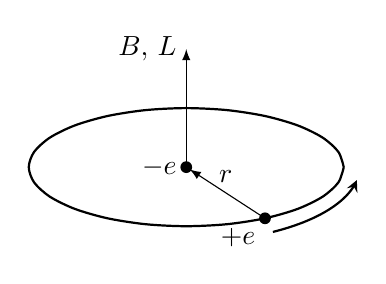
\begin{tikzpicture}[declare function={f(\x)=\ra*cos(\x) +\rb*sin(\x);}]
\pgfmathsetmacro{\ra}{2}
\pgfmathsetmacro{\rb}{0.75}
\pgfmathsetmacro{\rc}{\ra+0.2}
\pgfmathsetmacro{\rd}{\rb+0.2}
\draw[thick,domain=0:360]plot[smooth]({\ra*cos(\x)},{\rb*sin(\x)});
\draw [-latex] (0,0) node[left]{$-e$} node[fill=black, circle, inner sep=1.5pt]{} -- (0,1.5) node[left]{$\kvec{B}, \, \mat{L}$};
\draw [latex-,shorten <=1.5pt] (0,0) -- ({\ra*cos(300)},{\rb*sin(300)}) node[pos=0.5,above]{$r$} node[fill=black, circle, inner sep=1.5pt]{} node[below left]{$+e$};
\draw[-stealth,thick,domain=300:350]plot({\rc*cos(\x)},{\rd*sin(\x)});
\end{tikzpicture}
\caption{الیکٹران کے نقطہ نظر سے ہائیڈروجن جوہر۔}
\label{شکل_غیر_تابع_اضطراب_جوہر_الیکٹران_نقطہ_نظر}
\end{figure}

ہمیں پروٹان کا مقناطیسی میدان \عددی{(\kvec{B})}   اور الیکٹران کا جفت قطب معیار اثر \عددی{(\kvec{\mu})} درکار ہوگا۔ 

\quad
\موٹا{پروٹان کا مقناطیسی میدان۔}  ہم ( الیکٹران کے نقطہ نظر سے)  پروٹان کو استمراری دائری  رو (شکل \حوالہ{شکل_غیر_تابع_اضطراب_جوہر_الیکٹران_نقطہ_نظر})   تصور کرکے،  اس کے مقناطیسی میدان کو بایوٹ و سيوارٹ قانون سے حاصل کرتے ہیں :
\begin{align*} 
B = \frac{\mu_0 I}{2r}
\end{align*}
جس میں موثر رو \عددی{ I = e/T} ہے،  جہاں \عددی{ e} پروٹان کا بار،  اور \عددی{ T} دائرے پر ایک چکر کا دوری عرصہ  ہے۔  اس کے برعکس، \عددی{L = rmv = {2\pi m r ^2} /T}   ( مرکزہ کے ساکن  چھوکٹ میں)  الیکٹران کا مداری زاویائی معیار حرکت  ہوگا۔  مزید،  \عددی{ \kvec{B}} اور \عددی{\mat{L}} دونوں کا رخ ایک   جیسا ہوگا ( شکل \حوالہ{شکل_غیر_تابع_اضطراب_جوہر_الیکٹران_نقطہ_نظر} میں اوپر جانب)،  لہٰذا
\begin{align}\label{مساوات_غیر_مضطرب_اندرونی_مقناطیسی_میدان}
\kvec{B} = \frac{1}{4 \pi \epsilon_0} \frac{e}{mc^2 r^3} \mat{L}
\end{align}
لکھا جا سکتا ہے (جہاں میں نے \عددی{c = 1/\sqrt{\epsilon_0 \mu_0}} استعمال کرکے \عددی{\mu_0} کی جگہ \عددی{\epsilon_0} استعمال کیا ہے)۔ 

\quad
\موٹا{الیکٹران کا مقناطیسی جفت قطب معیار  حرکت۔}   چکر کھاتے بار کا مقناطیسی جفت قطب معیار اثر،  اس کے ( چکری)  زاویائی معیار حرکت سے تعلق رکھتا ہے؛   مسکن مقناطیسی  نسبت    ( جسے ہم   حصہ  \حوالہ{حصہ_تین_ابعاد_مقناطیسی_میدان_میں_ایک_الیکٹران}  میں دیکھ چکے ہیں)،   ان کے بیچ تناسبی جزو ضربی ہو گا۔  آئیں اس مرتبہ،   کلاسیکی برقی حرکیات استعمال کرتے ہوئے،  اسے اخذ کرتے ہیں۔ ایک ایسا بار \عددی{ q} جس کی لپائی  رداس \عددی{ r} کے چلا پر  کی گئی ہو،  اور جو محور کے گرد دوری عرصہ \عددی{ T} سے گھومتا ہو،  پر غور کریں(شکل  \حوالہ{شکل_غیر_تابع_اضطراب_چھلا_بار})۔   اس چھلے کے مقناطیسی جفت قطب معیار اثر کی تعریف،  رو \عددی{(q/T)} ضرب رقبہ \عددی{(\pi r^2)} ہے ۔
\begin{align*}
\mu = \frac{q \pi r^2}{T}
\end{align*}

\begin{figure}
\centering
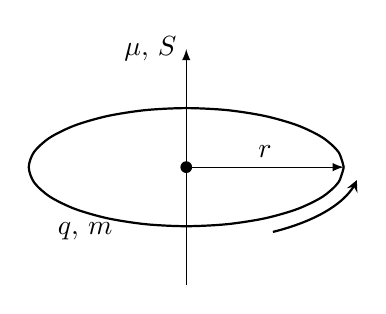
\begin{tikzpicture}[declare function={f(\x)=\ra*cos(\x) +\rb*sin(\x);}]
\pgfmathsetmacro{\ra}{2}
\pgfmathsetmacro{\rb}{0.75}
\pgfmathsetmacro{\rc}{\ra+0.2}
\pgfmathsetmacro{\rd}{\rb+0.2}
\draw[thick,domain=0:360]plot[smooth]({\ra*cos(\x)},{\rb*sin(\x)});
\draw [-latex] (0,-1.5) -- (0,1.5) node[left]{$\kvec{\mu}, \, \mat{S}$};
\draw [-latex] (0,0)node[circle,inner sep=1.5pt,fill=black]{} -- ({\ra*cos(0)},{\rb*sin(0)}) node[pos=0.5,above]{$r$};
\draw[-stealth,thick,domain=300:350]plot({\rc*cos(\x)},{\rd*sin(\x)});
\draw []  ({\ra*cos(230)},{\rb*sin(230)}) node[below]{$q,\, m$};
\end{tikzpicture}
\caption{بار کا چھلا جو اپنے محور کے گرد گھوم رہا ہے۔}
\label{شکل_غیر_تابع_اضطراب_چھلا_بار}
\end{figure}

اگر چھلے کی کمیت \عددی{ m} ہو،  جمودی معیار اثر \عددی{(mr^2)} ضرب زاویائی سمتی رفتار \عددی{(2 \pi/T)} اس کا زاویائی معیار حرکت،\عددی{S}، ہوگا ۔
\begin{align*} 
S = \frac{2 \pi mr^2}{T}
\end{align*}
اس  تشکیل   کے لیے ظاہر ہے کہ مسکن مقناطیسی نسبت \عددی{\mu /S = q/2m} ہوگا۔  دھیان رہے کہ یہ \عددی{ r} ( اور \عددی{ T})  کا  تابع نہیں  ہے۔  اگر میرے پاس کوئی زیادہ پیچیدہ شکل  کا جسم ہوتا،  مثلاً   ایک  کرہ (  صرف اتنا ضروری ہے کہ یہ اپنے محور کے گرد گھومتا ہوا  شکل طواف ہو)،   میں اس کو باریک چھلوں میں ٹکڑے کر کے،  تمام  چھلوں  کی  پیدا حصوں کا مجموعہ لے کر \عددی{\kvec{\mu}} اور \عددی{\mat{S}} کی قیمتیں معلوم کر پاتا۔ جب تک کمیت اور بار کی تقسیم ایک جیسی ہو ( تاکہ بار اور کمیت کی نسبت یکساں ہو)،  ہر  چھلے  کا اور لہٰذا   پورے جسم کا مسکن مقناطیسی نسبت ایک  جیسا ہوگا۔ مزید،  \عددی{\kvec{\mu}} اور \عددی{\mat{S}} کے رخ ایک  جیسے ( یا اگر بار منفی ہو تو ایک دونوں کے مخالف)  ہوں گے،  لہٰذا   درج ذیل ہوگا۔ 
\begin{align*}
\kvec{\mu} = \big ( \frac{q}{2m} \big ) \mat{S}
\end{align*}

یہ خالصاً  کلاسیکی حساب ہے، درحقیقت،  الیکٹران کا مقناطیسی معیار اثر اس کی  کلاسیکی قیمت کا دگنا ہے۔ 
\begin{align}\label{مساوات_غیر_مضطرب_جفت_قطب_معیار_اثر}
\kvec{\mu}_e = - \frac{e}{m} \mat{S}
\end{align}
ڈیراک   نے الیکٹران کی (اپنے)  اضافیتی نظریہ میں" اضافی"  جزو ضربی \عددی{2} کی وجہ پیش کی ہے۔\حاشیہد{ہم دیکھ چکے ہیں کہ الیکٹران کو  محور کے گرد چکر کاٹتا ہوا کرہ تصور کرنا،  خطرے سے باہر نہیں ہے (سوال \حوالہ{سوال_تین_ابعادی_بے_ساخت_ذرہ} دیکھیں)، اور یہ حیرت کی بات نہیں کہ سادہ لوح    کلاسیکی نمونہ،  مسکن مقناطیسی نسبت کی غلط قیمت دیتا ہے۔ کلاسیکی توقعات سے حاصل قیمت کو  \اصطلاح{\عددی{g} جزو ضربی}\فرہنگ{جی جزو ضربی}\فرہنگ{g-factor} کہتے ہیں: \عددی{\kvec{\mu}=g(q/2m)\kvec{S}}، لہٰذا    نظریہ ڈیراک میں \عددی{g} جزو ضربی کی قیمت ٹھیک \عددی{2} ہے۔لیکن \اصطلاح{ کوانٹائی برقی حرکیات }\فرہنگ{برقی حرکیات!کوانٹائی}\فرہنگ{electrodynamics!quantum} اس میں معمولی تصحیح دیتی ہے:  \اصطلاح{بے ضابطہ مقناطیسی معیار اثر}\فرہنگ{مقناطیسی معیار اثر!بے ضابطہ}\فرہنگ{magnetic moment!anomalous}،  \عددی{g_e}،  کی قیمت دراصل \عددی{2+(\alpha/\pi)+\dotsc=2.002\dotsc} ہے۔ اس کا حساب اور اس کی پیمائش (جو آپس میں شاندار    حتمیت تک متفق ہیں)  بیسویں صدی طبیعیات کی اہم ترین کامیابیوں میں سے ایک ہے۔}

 ان تمام کو اکٹھے کرتے ہوئے درج ذیل حاصل ہوگا ۔
\begin{align*}
H = \big ( \frac{e^2}{4 \pi \epsilon_0} \big ) \frac{1}{m^2 c^2 r^3} \mat{S} \cdot \mat{L}
\end{align*}
اس حساب میں ایک  فریب سے کام لیا گیا ہے:  میں نے الیکٹران کے ساکن  چھوکٹ میں تجزیہ کیا،  جو ایک غیر جمودی نظام ہے؛ چونکہ الیکٹران مرکزہ کے گرد گھومتا ہے، لہٰذا   یہ چھوکٹ  اسراع  پذیر ہوگا ۔اس حساب میں مجرد حرکیات تصحیح،  جسے \اصطلاح{ طامس استقبالی حرکت}\فرہنگ{طامس استقبالی حرکت}\حاشیہب{Thomas precession}\فرہنگ{Thomas precession} کہتے\حاشیہد{سوچنے کا ایک انداز یہ ہو گا کہ آپ تصور کریں کہ الیکٹران مستمر انداز میں  ایک ساکن نظام سے دوسرے ساکن نظام میں قدم رکھتا ہے؛  ان لورینز  تبادلہ کے مجموعی اثر کو طامس استقبالی حرکت بیان کرتا ہے۔ ہم تجربہ گاہ کی چھوکٹ میں، جہاں پروٹان ساکن ہے، رہ کر اس پوری   مصیبت سے نجات حاصل کر سکتے  تھے۔ ایسی صورت میں، پروٹان کا میدان خالصتاً برقی ہو گا، اور آپ سوچ سکتے ہیں کہ یہ الیکٹران پر قوت مروڑ کیسا پیدا کرتا ہے۔ حقیقت یہ ہے کہ حرکت پذیر  مقناطیسی جفت قطب، برقی جفت قطب معیار اثر اختیار کرتا ہے، اور تجربہ گاہ کے چھوکٹ میں مرکزہ کے  برقی میدان اور  الیکٹران کے  برقی جفت قطب معیار اثر کے بیچ باہم عمل،  چکر و مدار ربط کا باعث بنتا ہے۔ چونکہ اس  تجزیہ  کے لئے زیادہ پیچیدہ  برقی حرکیات درکار ہو گا  لہٰذا بہتر یہی ہے کہ ہم الیکٹران کے ساکن چھوکٹ میں کام کریں جہاں طبیعی   پہلو زیادہ واضح ہے۔ }  ہیں،    شامل کرکے قبول کیا جا سکتا ہے،  جو حساب میں جزو ضربی \عددی{1/2} شامل کرتا ہے۔\حاشیہد{یہ کہنا زیادہ درست ہو گا کہ  طامس استقبالی حرکت \عددی{g} جزو ضربی سے \عددی{1} منفی کرتا ہے۔} 
\begin{align}\label{مساوات_غیر_مضطرب_طامس_کا_کام}
H'_{so} = \big ( \frac{e^2}{8 \pi \epsilon_0} \big ) \frac{1}{m^2 c^2 r^3} \mat{S} \cdot \mat{L}
\end{align}
%=====================
یہ \اصطلاح{چکر و  مدار   باہم عمل}\فرہنگ{چکر و مدار باہم عمل}\حاشیہب{spin-orbit interaction}\فرہنگ{spin-orbit!interaction}  ہے؛  ماسوائے دو تصحیح (الیکٹران کی ترمیم شدہ مسکن مقناطیسی نسبت  اور طامس استقبالی حرکت جزو ضربی جو اتفاقاً ایک دوسرے کو کاٹتے  ہیں) کے،   یہ وہی نتیجہ ہے جو آپ  سادہ لوح   کلاسیکی نمونہ سے حاصل کرتے ہیں۔ طبیعی  طور پر،  یہ الیکٹران کے لمحاتی ساکن چھوکٹ  میں،  چکر کاٹتے ہوئے  الیکٹران کے مقناطیسی جفت قطب معیار اثر پر،   پروٹان کے مقناطیسی میدان  کی  قوت مروڑ کے  بدولت ہے۔

 اب کوانٹائی  میکانیات کی بات کرتے ہیں۔ چکر و دائری ربط کی صورت  میں \عددی{\mat{L}} اور \عددی{\mat{S}} کے ساتھ ہیملٹنی غیر مقلوب ہو گا،  لہٰذا چکر اور  مداری  زاویائی معیار اثر علیحدہ علیحدہ   بقائی  نہیں  ہوں گے   (سوال \حوالہ{سوال_غیر_مضطرب_بقائی_نہیں} دیکھیں)۔ البتہ،   \عددی{L^2}، \عددی{S^2} اور کل زاویائی معیار حرکت:
\begin{align}\label{مساوات_غیر_مضطرب_ایل_جمع_ایس_برابر_جے}
\mat{J} \equiv \mat{L} + \mat{S}
\end{align}
کے ساتھ \عددی{H'_{so}} مقلوب ہو گا،  لہٰذا   یہ مقداریں   بقائی  ہوں گی ( مساوات   \حوالہ{مساوات_قواعد_شرح_تبدیلی_قابل_مشاہدہ} اور اس کے نیچے پیراگراف دیکھیں )۔دوسرے لفظوں میں،  \عددی{L_z} اور \عددی{S_z} کے امتیازی حالات نظریہ اضطراب میں استعمال کے لئے "موزوں" حالات نہیں ہیں،  جبکہ \عددی{L^2}، \عددی{S^2}، \عددی{J^2}، اور \عددی{J_z} کے امتیازی حالات  "موزوں" حالات ہیں۔ اب 
\begin{align*}
J^2 = (\mat{L} + \mat{S}) \cdot (\mat{L} + \mat{S}) = L^2 + S^2 + 2 \mat{L} \cdot \mat{S}
\end{align*}
کی بنا پر 
\begin{align}
\mat{L} \cdot \mat{S} = \frac{1}{2} (J^2 - L^2 - S^2)
\end{align}
ہوگا  لہٰذا   \عددی{\mat{L} \cdot \mat{S}} کی  امتیازی اقدار درج ذیل ہوں گی ۔
\begin{align*}
\frac{\hslash^2}{2} [j (j + 1) - l(l + 1) - s(s + 1)]
\end{align*}
یہاں یقیناً \عددی{s = 1/2} ہے۔  مزید \عددی{1/r^3} کی توقعاتی قیمت  (سوال  \حوالہ{سوال_غیر_مضطرب_طاقتی_توقعاتی_قیمتیں}-ج  دیکھیں) 
\begin{align}\label{مساوات_غیر_مضطرب_آر_تین}
\big\langle \frac{1}{r^3} \big\rangle = \frac{1}{l(l + 1/2) (l + 1) n^3 a^3} 
\end{align}
 ہے، لہٰذا   
\begin{align*}
E_{so}^1 = \langle H'_{so} \rangle = \frac{e^2}{8 \pi \epsilon_0} \frac{1}{m^2 c^2} \frac{(\hslash^2 /2) [j(j + 1) - l(l + 1) - 3/4]}{l(l + 1/2)(l + 1)n^3 a^3}
\end{align*} 
  یا، تمام  کو  \عددی{E_n} کی صورت میں لکھتے ہوئے، درج ذیل اخذ کرتے ہیں۔ \حاشیہد{یہاں بھی، \عددی{l=0} کی صورت میں ہمیں  مسئلہ درپیش  ہو گا، چونکہ ہم بظاہر صفر سے تقسیم کرتے ہیں۔ ساتھ ہی، اس صورت میں \عددی{j=s} کی بنا پر،  شمار کنندہ بھی صفر ہے، لہٰذا مساوات \حوالہ{مساوات_غیر_مضطرب_چکر_و_مدار_ربط} بلا  تعیین ہو گا۔ طبیعی بنیادوں  پر \عددی{l=0} کی صورت میں چکر و مدار ربط ہونا ہی نہیں چاہیے۔ اس  ابہام کو دور کرنے کا ایک طریقہ یہ ہے کہ ہم \اصطلاح{جزو ڈارون}\فرہنگ{جزو ڈارون}\فرہنگ{Darwin term} متعارف کریں۔ غیر متوقع طور پر، اگرچہ اضافیتی تصحیح (مساوات \حوالہ{مساوات_غیر_مضطرب_اضافیتی_تصحیح}) اور چکر و مدار ربط (مساوات \حوالہ{مساوات_غیر_مضطرب_چکر_و_مدار_ربط}) دونوں \عددی{l=0} کی صورت میں شک سے مبرا نہیں ہیں، ان کا مجموعہ (مساوات \حوالہ{مساوات_غیر_مضطرب_اضافیتی_تصحیح_چکرومدار_ربط})  تمام \عددی{l} کے لئے درست ہے (سوال \حوالہ{سوال_غیر_مضطرب_ٹھیک_ٹھیک_جواب} دیکھیں)۔}
\begin{align}\label{مساوات_غیر_مضطرب_چکر_و_مدار_ربط}
E^1_{so} = \frac{(E_n)^2}{mc^2} \Big \{ \frac{n[j(j + 1) - l(l + 1) - 3/4]}{l(l + 1/2)(l + 1)} \Big \}
\end{align}

یہ ایک حیرت کن بات ہے کہ،  بالکل مختلف طبیعی پہلوؤں کے باوجود،  اضافیتی تصحیح (مساوات \حوالہ{مساوات_غیر_مضطرب_اضافیتی_تصحیح})  اور چکر و  مدار ربط (مساوات \حوالہ{مساوات_غیر_مضطرب_چکر_و_مدار_ربط})  ایک جتنا رتبہ \عددی{(E_n^2 / mc^2)} رکھتے ہیں۔ انہیں جمع کرکے،  ہمیں مکمل مہین ساخت  کلیہ:
\begin{align}\label{مساوات_غیر_مضطرب_اضافیتی_تصحیح_چکرومدار_ربط}
E_{fs}^1 = \frac{(E_n)^2}{2mc^2} \big ( 3 - \frac{4n}{j + 1/2} \big )
\end{align}
 ( سوال \حوالہ{سوال_غیر_مضطرب_مکمل_مہین_ساخت_کلیہ} دیکھیں)   حاصل ہوتا ہے ۔ اسے  کلیہ بوہر کے ساتھ ملا  کر،  ہم ہائیڈروجن  توانائی سطحوں کا عظیم نتیجہ:
\begin{align}\label{مساوات_غیر_مضطرب_مجموعی_نتیجہ_مہین}
E_{nj} = - \frac{\SI{13.6}{\electronvolt}}{n^2} \big [ 1 + \frac{\alpha^2}{n^2} \big ( \frac{n}{j + 1/2} - \frac{3}{2} \big ) \big ]
\end{align}
حاصل کرتے ہیں، جس میں مہین ساخت شامل ہے ۔ 

مہین ساخت \عددی{l} میں انحطاط  توڑتی ہے ( یعنی کسی ایک \عددی{ n} کیلئے،  \عددی{l} کی مختلف اجازتی قیمتیں ایک  جیسی توانائی کے حامل نہیں ہونگی)،  تاہم اب بھی یہ \عددی{ j} میں انحطاط  برقرار رکھتی  ہے ( شکل \حوالہ{شکل_غیر_مضطرب_ہائیڈروجن_سطح_توانائی}  دیکھیں)۔ مدارچی  اور چکری  زاویائی معیار حرکت  کے \عددی{ z} جزو امتیازی اقدار ( \عددی{m_l} اور \عددی{m_s})  اب "موزوں" کوانٹائی  اعداد نہیں ہونگے؛  ان مقداروں کی مختلف قیمتوں والے حالات کے خطی جوڑ ساکن حالات ہوں گے؛ " ‏موزوں" کوانٹائی  اعداد \عددی{n}، \عددی{l}، \عددی{s}، \عددی{j}، اور \عددی{m_j} ہونگے ۔\حاشیہد{کسی \عددی{l} اور \عددی{s} کے لئے، \عددی{|jm_j\rangle} کو \عددی{|lm_l\rangle|sm_s\rangle} کا خطی جوڑ لکھنے کی خاطر ہمیں مناسب    کلیبش و  گورڈن عددی سر (مساوات \حوالہ{مساوات_تین_ابعادی_کلیبش_گورڈن_خطی_مجموعہ})   استعمال کرنے ہوں گے۔}
\begin{figure}
\centering
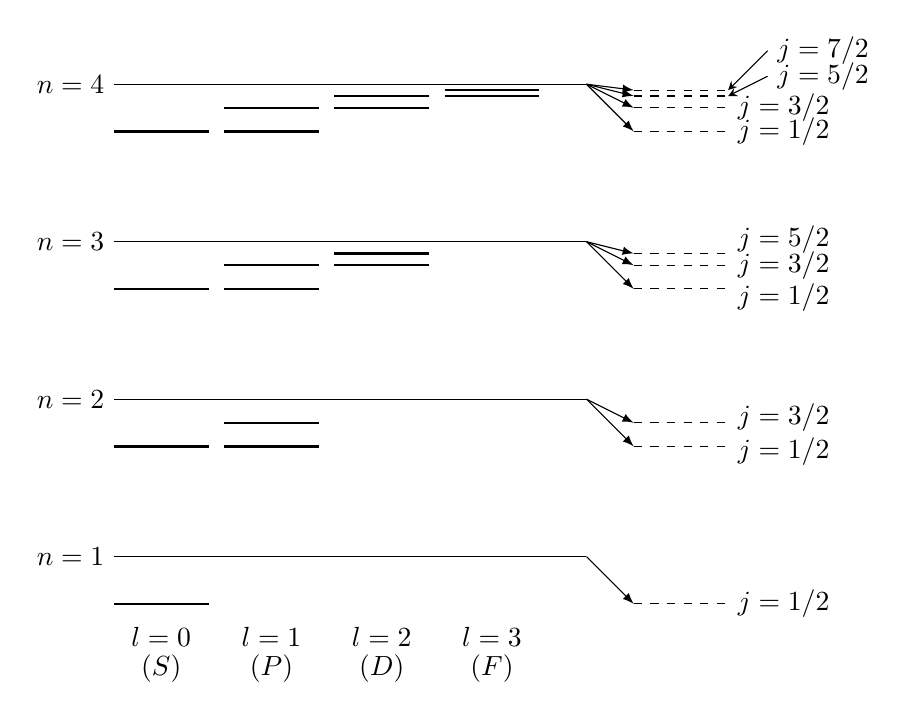
\begin{tikzpicture}
\pgfmathsetmacro{\da}{0.6}
\pgfmathsetmacro{\db}{\da/2}
\pgfmathsetmacro{\dc}{\db/2}
\pgfmathsetmacro{\dd}{\dc/2}
\pgfmathsetmacro{\stY}{2}
\pgfmathsetmacro{\dX}{0.2}
\pgfmathsetmacro{\stX}{1.2}
\pgfmathsetmacro{\Xmax}{6}
\pgfmathsetmacro{\arX}{0.6}
\draw(0,3*\stY)node[left]{$n=4$}--++(\Xmax,0)coordinate(kA);
\draw[thick](0,3*\stY-\da)--++(\stX,0);
\draw[thick](\stX+\dX,3*\stY-\da)--++(\stX,0);
\draw[thick](\stX+\dX,3*\stY-\db)--++(\stX,0);
\draw[thick](2*\stX+2*\dX,3*\stY-\db)--++(\stX,0);
\draw[thick](2*\stX+2*\dX,3*\stY-\dc)--++(\stX,0);
\draw[thick](3*\stX+3*\dX,3*\stY-\dc)--++(\stX,0);
\draw[thick](3*\stX+3*\dX,3*\stY-\dd)--++(\stX,0);
\draw[-latex](kA)--++(\arX,-\da)coordinate(kAa);
\draw[dashed](kAa)--++(2*\arX,0)node[right]{$j=1/2$};
\draw[-latex](kA)--++(\arX,-\db)coordinate(kAa);
\draw[dashed](kAa)--++(2*\arX,0)node[right]{$j=3/2$};
\draw[-latex](kA)--++(\arX,-\dc)coordinate(kAa);
\draw[dashed](kAa)--++(2*\arX,0)coordinate(kT);
\draw[stealth-](kT)--++(0.5,0.25)node[right]{$j=5/2$};
\draw[-latex](kA)--++(\arX,-\dd)coordinate(kAa);
\draw[dashed](kAa)--++(2*\arX,0)coordinate(kT);
\draw[stealth-](kT)--++(0.5,0.5)node[right]{$j=7/2$};
%
\draw(0,2*\stY)node[left]{$n=3$}--++(\Xmax,0)coordinate(kA);
\draw[thick](0,2*\stY-\da)--++(\stX,0);
\draw[thick](\stX+\dX,2*\stY-\da)--++(\stX,0);
\draw[thick](\stX+\dX,2*\stY-\db)--++(\stX,0);
\draw[thick](2*\stX+2*\dX,2*\stY-\db)--++(\stX,0);
\draw[thick](2*\stX+2*\dX,2*\stY-\dc)--++(\stX,0);
\draw[-latex](kA)--++(\arX,-\da)coordinate(kAa);
\draw[dashed](kAa)--++(2*\arX,0)node[right,yshift=-0.3em]{$j=1/2$};
\draw[-latex](kA)--++(\arX,-\db)coordinate(kAa);
\draw[dashed](kAa)--++(2*\arX,0)node[right]{$j=3/2$};
\draw[-latex](kA)--++(\arX,-\dc)coordinate(kAa);
\draw[dashed](kAa)--++(2*\arX,0)node[right,yshift=0.5em]{$j=5/2$};
%
\draw(0,\stY)node[left]{$n=2$}--++(\Xmax,0)coordinate(kA);
\draw[thick](0,1*\stY-\da)--++(\stX,0);
\draw[thick](\stX+\dX,1*\stY-\da)--++(\stX,0);
\draw[thick](\stX+\dX,1*\stY-\db)--++(\stX,0);
\draw[-latex](kA)--++(\arX,-\da)coordinate(kAa);
\draw[dashed](kAa)--++(2*\arX,0)node[right,yshift=-0.2em]{$j=1/2$};
\draw[-latex](kA)--++(\arX,-\db)coordinate(kAa);
\draw[dashed](kAa)--++(2*\arX,0)node[right,yshift=0.2em]{$j=3/2$};
%
\draw(0,0*\stY)node[left]{$n=1$}--++(\Xmax,0)coordinate(kA);
\draw[thick](0,0*\stY-\da)--++(\stX,0);
\draw[-latex](kA)--++(\arX,-\da)coordinate(kAa);
\draw[dashed](kAa)--++(2*\arX,0)node[right]{$j=1/2$};
%
\draw(\stX/2,-\da)node[below,yshift={-0.5em}]{$l=0$}node[below,yshift=-1.5em]{$(S)$};
\draw(\stX+\dX+\stX/2,-\da)node[below,yshift={-0.5em}]{$l=1$}node[below,yshift=-1.5em]{$(P)$};
\draw(2*\stX+2*\dX+\stX/2,-\da)node[below,yshift={-0.5em}]{$l=2$}node[below,yshift=-1.5em]{$(D)$};
\draw(3*\stX+3*\dX+\stX/2,-\da)node[below,yshift={-0.5em}]{$l=3$}node[below,yshift=-1.5em]{$(F)$};
\end{tikzpicture}
\caption{ہائیڈروجن کی سطحیں توانائی، جن میں مہین ساخت شامل ہے (درست پیمانہ کے مطابق نہیں ہے)۔}
\label{شکل_غیر_مضطرب_ہائیڈروجن_سطح_توانائی}
\end{figure}


\ابتدا{سوال}\شناخت{سوال_غیر_مضطرب_بقائی_نہیں}
درج ذیل مقلب کی قیمتیں تلاش کریں۔
 ( الف) \عددی{[\mat{L} \cdot \mat{S}, \mat{L}]}، ( ب) \عددی{[\mat{L} \cdot \mat{S}, \mat{S}]}،
  ( ج) \عددی{[\mat{L} \cdot \mat{S}, \mat{J}]}، ( د) \عددی{[\mat{L} \cdot \mat{S}, L^2]}،
   ( ه) \عددی{[\mat{L} \cdot \mat{S}, S^2]}، ( و) \عددی{[\mat{L} \cdot \mat{S}, J^2]}؛
   \ترچھا{ اشارہ:}  \عددی{\mat{L}} اور \عددی{\mat{S}} زاویائی معیار حرکت کے بنیادی مقلبیت رشتوں  (مساوات  \حوالہ{مساوات_تین_ابعادی_بنیادی_مقلبیت_رشتہ}  اور مساوات \حوالہ{مساوات_تین_ابعادی_بنیادی_مقلبی_رشتے}) کو مطمئن کرتے ہیں،  لیکن یہ ایک دوسرے کے ساتھ مقلوب ہیں۔ 
\انتہا{سوال}
\ابتدا{سوال}\شناخت{سوال_غیر_مضطرب_مکمل_مہین_ساخت_کلیہ}
اضافیتی تصحیح (مساوات \حوالہ{مساوات_غیر_مضطرب_اضافیتی_تصحیح})  اور چکر و مدار  ربط (مساوات  \حوالہ{مساوات_غیر_مضطرب_چکر_و_مدار_ربط})سے مہین ساخت کلیہ  (مساوات \حوالہ{مساوات_غیر_مضطرب_اضافیتی_تصحیح_چکرومدار_ربط})  اخذ  کریں۔ \ترچھا{ اشارہ:} دھیان رہے کہ \عددی{j = l \pm 1/2 }  (مساوات \حوالہ{مساوات_غیر_مضطرب_ایل_جمع_ایس_برابر_جے})ہے؛  مثبت  اور منفی علامت کو باری باری لیں، آپ دیکھیں گے کہ دونوں صورتوں میں  ایک    جیسا نتیجہ حاصل  ہوگا۔ 
\انتہا{سوال} 
\ابتدا{سوال}
 ہائیڈروجن     طیف  کے مرئی خطہ میں   سرخ  بالمر لکیر نمایاں ترین  ہے،  جو \عددی{n = 3} سے \عددی{n = 2} میں منتقلی سے پیدا ہوتی ہے۔سب سے پہلے،  اس طیفی  لکیر کا طول موج اور تعدد بوہر نظریہ سے تعین کریں۔  مہین ساخت اس لکیر کو قریب قریب کئی لکیروں میں تقسیم کرتی ہے؛   اب ایک سوال  پیدا ہوتا ہے: لکیروں کی تعداد کیا ہو گی  اور ان  کے بیچ فاصلہ کتنا ہو گا؟ \ترچھا{ اشارہ:}  پہلے قدم میں،  معلوم کریں کہ \عددی{n = 2} سطح کتنے  ذیلی سطحوں میں تقسیم ہوگا،  اور ہر ایک کے لیے،  \عددی{\si{\electronvolt}} میں،  \عددی{E_{fs}^1} تلاش کریں۔  یہی کچھ \عددی{n = 3} کے لیے کریں۔ سطح توانائی کے شکل کا خاکہ بنا کر \عددی{n = 3} سے \عددی{n = 2} تک تمام   ممکنہ منتقلی دکھائیں۔ توانائی کا اخراج     ( نوریہ کی صورت میں) \عددی{(E_3 - E_2) + \Delta E} ہوگا،  جہاں پہلا جزو سب میں مشترک  جبکہ (مہین ساخت  کی پیدا)  \عددی{\Delta E} کی قیمت  ہر  منتقلی کے لئے بدلے گی۔        ہر منتقلی کے لئے \عددی{\Delta E} کو ( \عددی{\si{\electronvolt}} میں) تلاش         کریں۔  آخر میں،   تعدد  نوریہ  میں تبدیل کرکے،   ساتھ ساتھ طیفی لکیروں کے بیچ فاصلہ  (\عددی{\si{\hertz}} کی صورت   میں)  تعین کریں؛یہ    ہر لکیر  اور    غیر مضطرب لکیر  کے بیچ تعددی فاصلہ نہیں ( جو یقیناً،  قابل مشاہدہ نہیں)، بلکہ یہ ہر لکیر اور اس سے  اگلی لکیر کے بیچ تعددی فاصلہ ہوگا۔  آپ کا جواب درج ذیل روپ میں ہونا چاہیے:  "سرخ  بالمر لکیر \عددی{(؟؟؟)} لکیروں میں تقسیم ہوتا ہے۔  بڑھتے تعدد کے لحاظ سے یہ \عددی{(1)} \عددی{j = (???)} سے \عددی{j = (???)}، \عددی{2} \عددی{j = (???)} سے \عددی{j = (???)}، \عددی{\dotsc} ہونگے۔  لکیر \عددی{1} اور لکیر \عددی{2} کے بیچ  تعددی فاصلہ \عددی{(???)} \عددی{\si{\hertz}} ہے،  لکیر \عددی{2} اور لکیر \عددی{3} کے بیچ فاصلہ \عددی{???} \عددی{\si{\hertz}} ہے،  \عددی{\dotsc} ۔"
\انتہا{سوال}
\ابتدا{سوال}\شناخت{سوال_غیر_مضطرب_ٹھیک_ٹھیک_جواب}
مساوات  ڈیراک  سے (نظریہ اضافت استعمال کیے بغیر )   ہائیڈروجن کے  مہین ساخت کا ٹھیک ٹھیک کلیہ درج ذیل حاصل ہوتا ہے ۔
\begin{align*}
E_{nj} = mc^2 \Big \{ \big [ 1 + \big ( \frac{\alpha}{n - (j + 1/2 ) + \sqrt{(j +1/2)^2 - \alpha^2}} \big )^2 \big ]^{- 1/2} -1 \Big \}
\end{align*}
 اس کو (یہ   جانتے ہوئے کہ \عددی{\alpha \ll 1} ہے)  \عددی{a^4} رتبہ تک پھیلا کر دکھائیں کہ  مساوات \حوالہ{مساوات_غیر_مضطرب_مجموعی_نتیجہ_مہین}  حاصل ہوتا ہے۔ 
\انتہا{سوال} 
%===========================


\حصہ{زیمان اثر} 
ایک جوہر کو یکساں بیرونی مقناطیسی میدان \عددی{\kvec{B}_{\text{بیرونی}}} میں رکھنے سے،  اس کی توانائی  سطحوں  میں تبدیلی پیدا ہوتی ہے۔ اس مظہر کو \اصطلاح{ زیمان اثر}\فرہنگ{زیمان اثر}\حاشیہب{Zeeman effect}\فرہنگ{Zeeman effect}  کہتے ہیں۔ واحد ایک الیکٹران کے لیے اضطراب درج ذیل ہوگا 
\begin{align} 
H'_z = - (\kvec{\mu}_l + \kvec{\mu}_s) \cdot \kvec{B}_{\text{بیرونی}}
\end{align}
جہاں 
\begin{align}
\kvec{\mu}_s = - \frac{e}{m} \mat{S}
\end{align}
الیکٹران چکر کے ساتھ وابستہ مقناطیسی جفت قطب معیار اثر،  اور 
\begin{align} 
\kvec{\mu}_l = - \frac{e}{2m} \mat{L}
\end{align}
مداری حرکت کے ساتھ وابستہ جفت قطب معیار اثر ہے۔  \حاشیہد{مداری حرکت کے لئے  کلاسیکی قیمت \عددی{(q/2m)} ہی  مسکن مقناطیسی نسبت  ہو گی؛ صرف  \ترچھا{چکر}  کی صورت میں \عددی{2} کا" اضافی" جزو ضربی پایا جاتا ہے۔} یوں  درج ذیل ہوگا ۔
\begin{align}
H_z' = \frac{e}{2m} (\mat{L} + 2 \mat{S}) \cdot \kvec{B}_{\text{بیرونی}}
\end{align}

زیمان تقسیم کی فطرت فیصلہ کن حد تک اندرونی میدان( مساوات  \حوالہ{مساوات_غیر_مضطرب_اندرونی_مقناطیسی_میدان})،    جو چکر و  مدار ربط پیدا کرتا ہے،  کے لحاظ سے بیرونی میدان کی طاقت پر منحصر ہوگی۔  اگر  \عددی{B_{\text{بیرونی}} \ll B_{\text{اندرونی}}} ہو تب مہین ساخت غالب ہوگی،  اور \عددی{H'} کو ایک چھوٹا اضطراب تصور کیا جا سکتا ہے، 
 جبکہ \عددی{B_{\text{بیرونی}} \gg B_{\text{اندرونی}}} کی صورت میں زیمان  اثر غالب ہوگا،  اور مہین ساخت  اضطراب تصور کی جائے گی۔  ان  خطوں کے بیچ،  جہاں دونوں میدان  مد مقابل   ہوں گے،  ہمیں انحطاطی نظریہ اضطراب کی پوری قوت درکار ہوگی، اور  ہیملٹنی کے  متعلقہ حصے کو " ہاتھ سے"  وتری بنانا لازم ہو گا۔ درج ذیل حصوں میں  ہائیڈروجن کے لئے  ہم ان تینوں  صورتوں   پر  غور کریں گے۔
  
\ابتدا{سوال} 
 ہائیڈروجن کی اندرونی میدان کی اندازاً  قیمت، مساوات \حوالہ{مساوات_غیر_مضطرب_اندرونی_مقناطیسی_میدان}  استعمال کرتے ہوئے،  تلاش کرکے   "طاقتور" اور "کمزور"  زیمان میدان  کی  مقداری    تصویر کشی کریں ۔
\انتہا{سوال} 

\جزوحصہ{کمزور میدان زیمان اثر}
اگر \عددی{B_{\text{بیرونی}} \ll B_{\text{اندرونی}}} ہو تب مہین ساخت  (مساوات \حوالہ{مساوات_غیر_مضطرب_مجموعی_نتیجہ_مہین})  غالب ہوگی، اور  "موزوں" کوانٹائی  اعداد \عددی{n}، \عددی{l}، \عددی{j}، اور \عددی{m_j} ہونگے ( تاہم،  چکر و مدار ربط کی موجودگی میں \عددی{\mat{L}} اور \عددی{\mat{S}} علیحدہ علیحدہ بقائی نہیں ہونگے،  لہٰذا \عددی{m_l} اور \عددی{m_s} " موزوں" کوانٹائی  اعداد نہیں ہونگے)۔\حاشیہد{یہاں ایک اضطراب (زیمان بٹوارا) کے اوپر دوسرا اضطراب (مہین ساخت)  انبار ہے۔"موزوں" کوانٹائی اعداد وہ ہوں گے جو غالب اضطراب، جو موجودہ  مسئلہ میں مہین ساخت ہے، کے لئے درست ہوں۔ثانوی اضطراب (زیمان بٹوارا)  \عددی{J_z} میں،جو یہاں حصہ \حوالہ{حصہ_غیر_مضطرب_دو_پڑتا_انحطاط} میں پیش کئے گئے مسئلہ میں  عامل \عددی{A} کا کردار ادا کرتا ہے،  باقی انحطاط اٹھاتا  ہے۔عامل \عددی{J_z} تکنیکی لحاظ سے \عددی{H_Z'} کے ساتھ غیر  مقلوبی  ہے، تاہم مساوات \حوالہ{مساوات_غیر_مضطرب_وقتی_اوسط} کی وقتی اوسط نقطہ نظر سے یہ مقلوبی ہوں  گے۔ }  رتبہ اول نظریہ اضطراب میں توانائی میں زیمان تصحیح درج ذیل ہوگی۔ 
\begin{align}\label{مساوات_غیر_مضطرب_کمزور_میدان_زیمان_تصحیح}
E_Z^1 = \langle nljm_j | H'_Z | nljm_j \rangle = \frac{e}{2m} \kvec{B}_{\text{بیرونی}} \cdot \langle \mat{L} + 2 \mat{S} \rangle 
\end{align} 
اب \عددی{\mat{L} + 2 \mat{S} = \mat{J} + \mat{S}} ہوگا۔  بدقسمتی سے،  ہمیں \عددی{\mat{S}} کی توقعاتی قیمت فوری طور پر معلوم نہیں ہے۔ لیکن ہم درج ذیل طریقہ سے اسے جان سکتے ہیں:  کل زاویائی معیار حرکت \عددی{\mat{J} = \mat{L} + \mat{S}} ایک مستقل ہے (شکل  \حوالہ{شکل_غیر_تابع_چکرومدار_غیر_بقائی})؛ اس مقررہ سمتیہ کے گرد \عددی{\mat{L}} اور \عددی{\mat{S}} تیزی سے استقبالی حرکت کرتے ہیں۔ بالخصوص،  \عددی{\mat{J}} پر \عددی{\mat{S}} کی قائمہ تظلیل،  \عددی{\mat{S}} کی  (وقتی)  اوسط قیمت:
\begin{align}\label{مساوات_غیر_مضطرب_وقتی_اوسط}
\mat{S}_{\text{\RL{اوسط}}}= \frac{(\mat{S} \cdot \mat{J})}{J^2} \mat{J} 
\end{align}
ہو گی۔ لیکن  \عددی{\mat{L} = \mat{J} - \mat{S}} ہے،  لہٰذا \عددی{L^2 = J^2 + S^2 - 2 \mat{J} \cdot \mat{S}} اور یوں 
\begin{align}
\mat{S} \cdot \mat{J} = \frac{1}{2} (J^2 + S^2 - L^2) = \frac{\hslash^2}{2} [j(j + 1) + s(s + 1) - l(l + 1)]
\end{align}
ہو گا، جس سے درج ذیل حاصل ہوتا ہے ۔
\begin{align}
\langle \mat{L} + 2 \mat{S} \rangle =\Big \langle \big ( 1 + \frac{\mat{S} \cdot \mat{J}}{J^2} \big ) \mat{J} \Big\rangle = \Big [ 1 + \frac{j (j + 1) - l (l + 1) + 3/4}{2 j (j + 1)} \Big ] \langle \mat{J} \rangle
\end{align}
چوکور  قوسین   میں بند رکن کو \اصطلاح{ لنڈے \عددی{ g} جزو ضرب}\فرہنگ{لنڈے جی جزو ضربی}\حاشیہب{Lande g-factor}\فرہنگ{Lande g-factor}   کہتے ہیں جس کو \عددی{g_J} سے ظاہر کیا جاتا ہے۔

 ہم محور \عددی{z} کو \عددی{\kvec{B}_{\text{بیرونی}}} کے ساتھ ساتھ رکھ سکتے ہیں؛  تب 
\begin{align}\label{مساوات_غیر_مضطرب_زیمان_حصہ}
E_Z^1 = \mu_B g_J B_{\text{بیرونی}} m_j
\end{align}
ہو گا، جہاں 
\begin{align}
\mu_B \equiv \frac{e \hslash}{2m} = \SI{5.788e-5}{\electronvolt\per T}
\end{align}
\اصطلاح{بوہر مقناطیسہ}\فرہنگ{بوہر مقناطیسہ}\حاشیہب{Bohr magneton}\فرہنگ{Bohr magneton}  کہلاتا ہے۔ مہین ساخت  (مساوات  \حوالہ{مساوات_غیر_مضطرب_مجموعی_نتیجہ_مہین})  اور زیمان   ( مساوات \حوالہ{مساوات_غیر_مضطرب_زیمان_حصہ})   حصوں  کا مجموعہ کل توانائی   دے گا۔  مثال کے طور پر،  زمینی حال ( \عددی{n = 1}، \عددی{l = 0}، \عددی{j = 1/2} لہٰذا \عددی{g_J = 2})  دو سطحوں:
\begin{align}
\underbrace{\SI{- 13.6}{\electronvolt} (1 + \alpha^2 /4)}_{\text{\RL{مساوات \حوالہ{مساوات_غیر_مضطرب_مجموعی_نتیجہ_مہین}}}}\,\underbrace{ \pm \mu_B B_{\text{بیرونی}}}_{\text{\RL{مساوات \حوالہ{مساوات_غیر_مضطرب_زیمان_حصہ}}}}
\end{align}
 میں  بٹ  جائے گا ، جہاں \عددی{m_j = 1/2} کے لیے مثبت علامت اور \عددی{m_j = -1/2} کے لیے منفی علامت استعمال ہوگی۔ ان توانائیوں کو ( \عددی{B_{\text{بیرونی}}} کے تفاعل کے طور پر)  شکل   \حوالہ{شکل_غیر_تابع_اضطراب_زیمان_بٹوارا_کمزور_میدان}  میں  ترسیم کیا گیا ہے۔
\begin{figure}
\centering
\pgfmathsetmacro{\ra}{2}
\pgfmathsetmacro{\rb}{0.75}
\begin{tikzpicture}[declare function={f(\x)=\ra*cos(\x); g(\x)=\rb*sin(\x);}]
\draw[rotate around={-45:(0,0)}, domain=0:360] plot[smooth] ({f(\x)},{g(\x)});
\draw[rotate around={-45:(0,0)}, -stealth](0,-3) node[fill=black,circle,inner sep=1.5pt]{} -- (0,0) node[pos=0.5, above left] {$\mat{J}$} node[fill=black,circle,inner sep=1.5pt]{} -- (0,2);
\draw[rotate around={-45:(0,0)}, -stealth] (0,-3) -- ({f(330)},{g(330)}) node[pos=0.5, below right]{$\mat{L}$};
\draw[rotate around={-45:(0,0)}, -stealth] ({f(330)},{g(330)}) -- (0,2) node[pos=0.75, above right]{$\mat{S}$};
\end{tikzpicture}
\caption{چکر و مدار ربط  کی عدم موجودگی میں \عددی{\mat{L}} اور \عددی{\mat{S}} علیحدہ علیحدہ  بقائی نہیں ہوں گے؛ یہ اٹل  کل  زاویائی معیار  حرکت \عددی{\mat{J}}  کے گرد استقبالی حرکت کرتے ہیں۔} 
\label{شکل_غیر_تابع_چکرومدار_غیر_بقائی}
\end{figure}

 
\ابتدا{سوال} \شناخت{سوال_غیر_مضطرب_کمزور_میدان_زیمان_اثر}
آٹھ عدد \عددی{n = 2} حالات \عددی{| 2ljm_j \rangle} پر غور کریں۔ کمزور میدان زیمان بٹوارے   کی صورت میں ہر  ایک حال کی توانائی تلاش کرکے شکل  \حوالہ{شکل_غیر_تابع_اضطراب_زیمان_بٹوارا_کمزور_میدان}  کی طرز کا خاکہ بنا کر دکھائیں \عددی{B_{\text{بیرونی}}} بڑھانے سے توانائیاں کس طرح ارتقا کرتی ہے۔  ہر خط کو نام دے کر اس کی ڈھلوان دکھائیں ۔
\begin{figure}
\centering
\begin{tikzpicture}
\pgfmathsetmacro{\a}{40}
\pgfmathsetmacro{\b}{180-\a}
\pgfmathsetmacro{\c}{0.4}
\draw[thick] (0,0) node[circle, fill=black, inner sep=1.5pt]{} --++ (-45:2.5) node[right]{$m_j = -1/2$};
\draw[thick] (0,0)node[left]{$-13.6(1+\alpha^2/4)\,\si{\electronvolt}$} --++ (45:2.5) node[right]{$m_j = 1/2$};
\draw(0,-1.5) -- (0,2) to [out=-\a, in =-\b] ++(\c,0) (0,2) to [out=\b, in =\a] ++(-\c,0) (0,2.15) to [out=-\a, in =-\b] ++(\c,0) (0,2.15) to [out=\b, in =\a] ++(-\c,0) ;
\draw[-latex](0,2.15) --++ (0,1) node[left]{$E$};
\draw[-latex](-0.5,2.5) --++ (4,0) node[above]{$\mu_B B_{\text{بیرونی}}$};
\end{tikzpicture}
\caption{ہائیڈروجن کے زمینی حال کا کمزور میدانی زیمان بٹوارا؛ بالائی  لکیر  \عددی{(m_j=1/2)} کی ڈھلوان \عددی{1} ہے؛ نچلی لکیر \عددی{(m_j=-1/2)} کی ڈھلوان \عددی{-1} ہے۔}
\label{شکل_غیر_تابع_اضطراب_زیمان_بٹوارا_کمزور_میدان}
\end{figure}


\انتہا{سوال} 


\جزوحصہ{طاقتور میدان زیمان اثر}
اگر \عددی{B_{\text{بیرونی}} \gg B_{\text{اندرونی}}} ہو،   تب  زیمان  اثر غالب ہوگا؛ \حاشیہد{ایسی صورت میں زیمان اثر کو   \اصطلاح{پاشن و بیک اثر}\فرہنگ{پاشن و بیک اثر}\فرہنگ{Paschen-Back effect} بھی کہتے ہیں۔} میدان \عددی{B_{\text{بیرونی}}} کو \عددی{ z} محور پر رکھ کر  "موزوں" کوانٹائی  اعداد \عددی{n}، \عددی{l}، \عددی{m_l}، اور \عددی{m_s} ہونگے  ( جبکہ \عددی{ j} اور \عددی{m_j} نہیں ہونگے،  چونکہ بیرونی قوت مروڑ کی صورت میں کل زاویائی  معیار حرکت بقائی  نہیں ہوگا  ، جبکہ \عددی{L_z} اور \عددی{S_z} بقائی  ہونگے)۔  زیمان ہیملٹنی 
\begin{align*}
H'_Z = \frac{e}{2m} B_{\text{بیرونی}} (L_z + 2S_z)
\end{align*}
ہو گا، جبکہ " غیر مضطرب"  توانائیاں  درج ذیل ہوں گی۔ 
\begin{align}\label{مساوات_غیر_مضطرب_طاقتور_زیمان_حصہ}
E_{nm_lm_s} = - \frac{\SI{13.6}{\electronvolt}}{n^2} + \mu_B B_{\text{بیرونی}} (m_l + 2m_s)
\end{align}
مہین ساخت کو مکمل نظرانداز کرتے ہوئے یہی جواب ہوگا۔ تاہم ہم  اس سے بہتر  جواب حاصل کر سکتے ہیں۔

 رتبہ اول نظریہ اضطراب میں ان سطحوں کی مہین ساخت تصحیح درج ذیل ہوگی ۔
\begin{align}\label{مساوات_غیر_مضطرب_نظریہ_اضطراب_پہلی_تصحیح}
E_{fs}^1 = \langle nlm_l m_s | (H'_r + H'_{so}) | \rangle nlm_l m_s \rangle
\end{align}
اضافیتی حصہ وہی ہوگا جو پہلے تھا (مساوات\حوالہ{مساوات_غیر_مضطرب_اضافیتی_تصحیح})؛   چکر و مدار جزو  (مساوات \حوالہ{مساوات_غیر_مضطرب_طامس_کا_کام})   کے لیے ہمیں
\begin{align}\label{مساوات_غیر_مضطرب_نقطی_ضرب}
\langle \mat{S} \cdot \mat{L} \rangle = \langle S_x \rangle \langle L_x \rangle + \langle S_y \rangle \langle L_y \rangle + \langle S_z \rangle \langle L_z \rangle = \hslash^2 m_l m_s
\end{align}
درکار ہو گا (یاد  رہے  \عددی{S_z} اور \عددی{L_z} کے  امتیازی تفاعلات کے لیے \عددی{
\langle S_x \rangle = \langle S_y \rangle = \langle L_x \rangle = \langle Ly \rangle=0
} ہوگا)۔   ان تمام کو اکٹھے کرکے (سوال  \حوالہ{سوال_غیر_مضطرب_اکٹھے_تمام}) ہم درج ذیل اخذ کرتے ہیں ۔
\begin{align}\label{مساوت_غیر_مضطرب_طاقتور_مہین_ساخت_حصہ}
E_{fs}^1 = \frac{\SI{13.6}{\electronvolt}}{n^3} \alpha^2 \Big \{ \frac{3}{4n} - \Big [ \frac{l(l + 1) - m_l m_s}{l(l + 1/2)(l + 1)} \Big ] \Big\}
\end{align}
( چوکور  قوسین    میں جزو،   \عددی{l = 0} کے لئے بلا تعیین ہے؛  اس  صورت میں اس کی درست قیمت  \عددی{1}  ہے؛  سوال  \حوالہ{سوال_غیر_مضطرب_قیمت_اکائی}  دیکھیں۔) زیمان   (مساوات \حوالہ{مساوات_غیر_مضطرب_طاقتور_زیمان_حصہ})  اور مہین ساخت   (مساوات  \حوالہ{مساوت_غیر_مضطرب_طاقتور_مہین_ساخت_حصہ})    حصوں کا مجموعہ کل توانائی دے گا ۔
 
\ابتدا{سوال}\شناخت{سوال_غیر_مضطرب_اکٹھے_تمام}
مساوات  \حوالہ{مساوات_غیر_مضطرب_نظریہ_اضطراب_پہلی_تصحیح}  سے آغاز کر کے مساوات \حوالہ{مساوات_غیر_مضطرب_اضافیتی_تصحیح} ،  مساوات \حوالہ{مساوات_غیر_مضطرب_طامس_کا_کام}، مساوات \حوالہ{مساوات_غیر_مضطرب_آر_تین}، اور  مساوات \حوالہ{مساوات_غیر_مضطرب_نقطی_ضرب}  استعمال کرتے ہوئے مساوات\حوالہ{مساوت_غیر_مضطرب_طاقتور_مہین_ساخت_حصہ}  اخذ کریں ۔
\انتہا{سوال}
\ابتدا{سوال}\شناخت{سوال_غیر_مضطرب_طاقتور_میدان_زیمان}
آٹھ عدد \عددی{n = 2} حالات  \عددی{| 2l m_l m_s \rangle} پر غور کریں۔ طاقتور میدان زیمان بٹوارا  کی صورت میں ہر حال کی توانائی تلاش کریں۔  اپنے جواب کو بوہر توانائی،  (  \عددی{\alpha^2} کے راست متناسب)  مہین ساخت،  اور  ( \عددی{\mu_B B_{\text{بیرونی}}} کے راست متناسب)  زیمان حصہ کے مجموعہ کی صورت میں لکھیں۔ مہین  ساخت کو مکمل طور پر نظر انداز کرتے ہوئے،  منفرد سطحوں کی تعداد کتنی ہوگی،  اور ان کے انحطاط کیا ہوں گے؟ 
\انتہا{سوال}
\ابتدا{سوال}\شناخت{سوال_غیر_مضطرب_قیمت_اکائی}
اگر \عددی{l = 0} ہو،  تب \عددی{j = s}، \عددی{m_j = m_s} ہوگا،  اور  کمزور اور طاقتور دونوں میدانوں کے لیے موزوں حالات \عددی{(|nm_s \rangle)} ایک  جیسے ہوں گے۔( مساوات \حوالہ{مساوات_غیر_مضطرب_کمزور_میدان_زیمان_تصحیح} سے)  \عددی{E_Z^1} اور  (مساوات \حوالہ{مساوات_غیر_مضطرب_مجموعی_نتیجہ_مہین} سے)  مہین ساخت توانائیاں تعین کر کے،  میدان کی طاقت سے قطع نظر،  \عددی{l = 0}  زیمان اثر کا عمومی نتیجہ لکھیں۔ دکھائیں کہ   چوکور قوسین   رکن کی قیمت  \عددی{1} لیتے ہوئے،  طاقتور میدان کلیہ (مساوات  \حوالہ{مساوت_غیر_مضطرب_طاقتور_مہین_ساخت_حصہ})  یہی نتیجہ دے گا  ۔
\انتہا{سوال}
%============================


\جزوحصہ{درمیانہ میدان زیمان اثر} 
درمیانے میدان کی صورت میں  نہ  \عددی{H'_Z} اور نہ ہی \عددی{H'_{fs}} غالب ہوگا،  لہٰذا  ہمیں دونوں کو،  ایک نظر سے دیکھ کر،  بوہر ہیملٹنی (مساوات \حوالہ{مساوات_غیر_مضطرب_بوہر_ہیملٹنی}) کے اضطراب تصور کرنا ہوگا ۔
\begin{align}
H' = H'_Z + H'_{fs}
\end{align}
میں \عددی{n = 2} صورت پر اپنی توجہ محدود رکھ کر،  ان  حالات کو، جن کی تصویر کشی  \عددی{l}، \عددی{j}، اور \عددی{m_j}  کرتے ہیں،\حاشیہد{آپ چاہیں تو \عددی{l}، \عددی{m_l}، \عددی{m_s} حالات استعمال کر سکتے ہیں، جو \عددی{H_Z'} کے قالبی ارکان کا حصول آسان لیکن \عددی{H_{fs}'} کا زیادہ  مشکل  بناتے ہیں؛ قالب \عددی{\mat{W}} زیادہ پیچیدہ ہو گا، لیکن امتیازی اقدار (جو اساس  کی تابع  نہیں)  دونوں صورتوں میں ایک جیسی   ہوں گی۔}    انحطاطی نظریہ اضطراب کی  اساس لیتا ہوں۔  کلیبش و  گورڈن عددی سر (سوال \حوالہ{سوال_تین_ابعادی_کلیبش_گورڈن_عددی_سر_آدھا} یا جدول \حوالہ{جدول_تین_ابعادی_کلیبش_گورڈن_عددی_سر} )  استعمال کرتے   ہوئے \عددی{| j m_j \rangle } کو \عددی{| lm_l \rangle | sm_s \rangle} کا خطی جوڑ لکھ کر،  درج ذیل ہوگا ۔
\begin{align*}
l &= 0
\begin{cases}
\psi_1 \equiv | \frac{1}{2} \frac{1}{2} \rangle = | 00 \rangle | \frac{1}{2} \frac{1}{2} \rangle \\
\psi_2 \equiv | \frac{1}{2} \frac{-1}{2} \rangle = | 00 \rangle | \frac{1}{2} \frac{-1}{2} \rangle
\end{cases} \\
l &= 1
\begin{cases}
\psi_3 \equiv | \frac{3}{2} \frac{3}{2} \rangle = | 11 \rangle | \frac{1}{2} \frac{1}{2} \rangle \\
\psi_4 \equiv | \frac{3}{2} \frac{-3}{2} \rangle = | 1 - 1 \rangle | \frac{1}{2} \frac{-1}{2} \rangle \\
\psi_5 \equiv | \frac{3}{2} \frac{1}{2} \rangle = \sqrt{2/3}| 10 \rangle | \frac{1}{2} \frac{1}{2} \rangle + \sqrt{1/3} | 11 \rangle \frac{1}{2} \frac{-1}{2} \rangle \\
\psi_6 \equiv | \frac{1}{2} \frac{1}{2} \rangle = - \sqrt{1/3} | 10 \rangle | \frac{1}{2} \frac{1}{2} \rangle + \sqrt{2/3} | 11 \rangle \frac{1}{2} \frac{-1}{2} \rangle \\
\psi_7 \equiv | \frac{3}{2} \frac{-1}{2} \rangle = \sqrt{1/3} | 1 - 1 \rangle | \frac{1}{2} \frac{1}{2} \rangle + \sqrt{2/3} | 10 \rangle \frac{1}{2} \frac{-1}{2} \rangle \\
\psi_8 \equiv | \frac{1}{2} \frac{-1}{2} \rangle = - \sqrt{2/3} | 1 - 1 \rangle | \frac{1}{2} \frac{1}{2} \rangle + \sqrt{1/3} | 10 \rangle \frac{1}{2} \frac{-1}{2} \rangle
\end{cases}
\end{align*}

اس اساس میں \عددی{H'_{fs}} کے تمام غیر صفر  قالبی ارکان،  جنہیں مساوات \حوالہ{مساوات_غیر_مضطرب_اضافیتی_تصحیح_چکرومدار_ربط}  دیتی ہے،  وتر پر ہوں گے؛  \عددی{H'_Z} کے چار غیر وتری ارکان پائے جاتے ہیں،  اور  مکمل قالب  \عددی{W}  (سوال  \حوالہ{سوال_غیر_مضطرب_مکمل_قالب}  دیکھیں) درج ذیل ہوگا  
\begin{align*}
\begin{pmatrix}
5 \gamma - \beta & 0 & 0 & 0 & 0 & 0 & 0 & 0 \\
0 & 5 \gamma + \beta & 0 & 0 & 0 & 0 & 0 & 0 \\
0 & 0 & \gamma - 2 \beta & 0 & 0 & 0 & 0 & 0 \\
0 & 0 & 0 &  \gamma + 2 \beta & 0 & 0 & 0 & 0 \\
0 & 0 & 0 & 0 & \gamma - \tfrac{2}{3} \beta & \tfrac{\sqrt{2}}{3} \beta & 0 & 0 \\
0 & 0 & 0 & 0 & \tfrac{\sqrt{2}}{3} \beta & 5 \gamma - \tfrac{1}{3} \beta & 0 & 0 \\
0 & 0 & 0 & 0 & 0 & 0 & \gamma + \tfrac{2}{3} \beta & \tfrac{\sqrt{2}}{3} \beta \\
0 & 0 & 0 & 0 & 0 & 0 & \tfrac{\sqrt{2}}{3} \beta & 5 \gamma + \tfrac{1}{3} \beta 
\end{pmatrix}
\end{align*}
جہاں درج ذیل ہوں گے ۔
\begin{align*}
\gamma \equiv (\alpha /8)^2 \SI{13.6}{\electronvolt} \quad \text{\RL{اور}} \quad \beta \equiv \mu_B \kvec{B}_{\text{بیرونی}}
\end{align*}
ابتدائی چار امتیازی اقدار پہلے سے وتر پر دکھائے گئے ہیں؛  اب صرف دو \عددی{2 \times 2} ڈبوں کی امتیازی اقدار تلاش کرنا باقی ہے۔ ان میں سے پہلی کی امتیازی مساوات درج ذیل ہے 
\begin{align*}
\lambda^2 - \lambda (6 \gamma - \beta) + \big ( 5 \gamma^2 - \frac{11}{3} \gamma \beta \big ) = 0
\end{align*}
جس سے دو درجی کلیہ درج ذیل امتیازی اقدار دے گا ۔
\begin{align}
\lambda_{\pm} = - 3 \gamma + (\beta /2) \pm \sqrt{4 \gamma^2 + (2/3) \gamma \beta + (\beta^2 /4)}
\end{align}
دوسرے ڈبے کی امتیازی اقدار یہی مساوات دے گی، لیکن اس میں \عددی{\beta} کی علامت الٹ ہوگی۔ ان آٹھ توانائیوں کو جدول \حوالہ{جدول_غیر_مضطرب_سطحیں_توانائی_برائے_دو} میں پیش کیا گیا ہے،  اور   شکل  \حوالہ{شکل_غیر_تابع_اضطراب_کمزور_درمیانہ_طاقتور}  میں \عددی{B_{\text{بیرونی}}} کے لحاظ سے ترسیم کیا گیا ہے۔ صفر میدان حد \عددی{(\beta = 0)} میں یہ گھٹ کر  مہین ساخت قیمتیں دیتی ہیں؛  کمزور میدان \عددی{(\beta \ll \gamma)}  میں یہ سوال \حوالہ{سوال_غیر_مضطرب_کمزور_میدان_زیمان_اثر}  میں حاصل نتائج دیتی ہیں؛  طاقتور
 میدان  \عددی{(\beta \gg \gamma)}  میں   سوال  \حوالہ{سوال_غیر_مضطرب_طاقتور_میدان_زیمان} کے نتائج حاصل ہوتے ہیں ( دھیان رہے،  جیسا سوال \حوالہ{سوال_غیر_مضطرب_طاقتور_میدان_زیمان} میں پیشنگوئی کی گئی، بہت زیادہ طاقتور میدانوں میں  پانچ منفرد  سطح توانائی  پر ارتکاز ہو گا) ۔
\begin{figure}
\centering
\begin{tikzpicture}
\draw[-stealth] (0,0) -- (5.5,0) node[below]{$\mu_B B_{\text{بیرونی}}$};
\draw[-stealth] (0,0) -- (0,5.5) node[left]{$E$};
\draw[](0,2.5) node[left]{$0$} --++ (0.1,0);
\draw[thick](0,2.6) -- (5,0.2);
\draw[thick](0,2.6) to [out=-10,in=175] (5,2.0);
\draw[thick](0,2.6) to [out=5, in=-163] (5,3.7);
\draw[thick](0,2.6) -- (5,5);
\draw[thick, dashed](0,2.1) -- (5,0.6);
\draw[thick, dashed](0,2.1) -- (5,3.5);
\draw[thick](0,2.1) to [out=-5, in=160] (5,0.7);
\draw[thick](0,2.1) to [out=3, in=175] (5,1.95);
\draw[-stealth](0.25,5.25) -- (4.75,5.25) node[pos=0.1,fill=white]{کمزور} node[pos=0.4,fill=white]{درمیانہ} node[pos=0.75,fill=white]{طاقتور};
\end{tikzpicture}
\caption{کمزور، درمیانہ اور طاقتور میدان میں ہائیڈروجن کے  \عددی{n=2} حال کا  زیمان بٹوارا۔}
\label{شکل_غیر_تابع_اضطراب_کمزور_درمیانہ_طاقتور}
\end{figure}
%
\begin{table}
\caption{
مہین ساخت اور زیمان بٹوارا کے ساتھ،  ہائیڈروجن کے \عددی{n=2} حالات کی سطحیں توانائی۔
}
\label{جدول_غیر_مضطرب_سطحیں_توانائی_برائے_دو}
\centering
\renewcommand{\arraystretch}{1.5}
\begin{tabular}{L}
\toprule
\epsilon_1=E_2-5\gamma+\beta\\
\epsilon_2=E_2-5\gamma-\beta\\
\epsilon_3=E_2-\gamma+2\beta\\
\epsilon_4=E_2-\gamma-2\beta\\
\epsilon_5=E_2-3\gamma+\beta/2+\sqrt{4\gamma^2+(2/3)\gamma\beta+\beta^2/4}\\
\epsilon_6=E_2-3\gamma+\beta/2-\sqrt{4\gamma^2+(2/3)\gamma\beta+\beta^2/4}\\
\epsilon_7=E_2-3\gamma-\beta/2+\sqrt{4\gamma^2+(2/3)\gamma\beta+\beta^2/4}\\
\epsilon_8=E_2-3\gamma-\beta/2-\sqrt{4\gamma^2+(2/3)\gamma\beta+\beta^2/4}\\
\bottomrule
\end{tabular}
\end{table}

\ابتدا{سوال}\شناخت{سوال_غیر_مضطرب_مکمل_قالب}
قوالب  \عددی{H_Z'} اور \عددی{H'_{fs}} کے ارکان  دریافت کر کے،  \عددی{n=2} کے لئے، متن  میں دیا گیا قالب \عددی{W} مرتب کریں۔
\انتہا{سوال}
\ابتدا{سوال} 
ہائیڈروجن کے \عددی{n = 3} حالات کے لیے کمزور، طاقتور اور درمیانے میدان خطوں کے لیے  زیمان اثر کا تجزیہ کریں۔ (جدول \حوالہ{جدول_غیر_مضطرب_سطحیں_توانائی_برائے_دو} کی طرز پر)  توانائیوں کا جدول تیار کرکے،  انہیں (شکل \حوالہ{شکل_غیر_تابع_اضطراب_کمزور_درمیانہ_طاقتور} کی طرح) بیرونی میدان کے تفاعلات کے طور پر ترسیم کریں، اور  تصدیق کریں  کہ درمیانے میدان  نتائج دو تحدیدی صورتوں میں گھٹ کر  درست قیمتی دیتی ہیں۔  
\انتہا{سوال}

%===================
\جزوحصہ{نہایت مہین بٹوارا}
پروٹان خود ایک مقناطیسی جفت قطب  ہے،  اگرچہ نسب نما میں بڑی  کمیت کی بنا پر اس کا جفت قطب معیار اثر،  الیکٹران کے جفت قطب معیار اثر سے بہت کم ہوگا ( مساوات \حوالہ{مساوات_غیر_مضطرب_جفت_قطب_معیار_اثر})۔ 
\begin{align}
\kvec{\mu}_p = \frac{g_p e}{2 m_p} \mat{S}_p, \quad \kvec{\mu}_e = - \frac{e}{m_e} \mat{S}_e
\end{align}
(پروٹان  تین کوارکوں پر مشتمل  مخلوط ساخت کا ذرہ ہے،       اور اس کی مسکن مقناطیسی نسبت الیکٹران کی مسکن مقناطیسی نسبت کی طرح سادہ نہیں؛ اسی لئے     \عددی{g} جزو ضربی کو  \عددی{g_p} لکھا گیا ہے،  جس کی پیمائشی قیمت \عددی{5.59}  ہے جو الیکٹران کی قیمت \عددی{(2)} سے مختلف ہے۔ ) کلاسیکی برقی حرکیات کے تحت، جفت قطب  \عددی{\kvec{\mu}} درج ذیل مقناطیسی میدان پیدا کرتا ہے ۔\حاشیہد{اگر آپ  مساوات \حوالہ{مساوات_غیر_مضطرب_پروٹان_میدان} میں مستعمل ڈیلٹا تفاعلی جزو سے واقف نہیں، جفت قطب کو   چکر کاٹتا ہوا بار دار کروی  خول   تصور کرکے،(\عددی{\kvec{\mu}} کو برقرار رکھ کر)  رداس کو صفر تک اور بار کو لامتناہی تک پہنچا کر، آپ اس کو اخذ کر سکتے ہیں۔ }
\begin{align}\label{مساوات_غیر_مضطرب_پروٹان_میدان}
\kvec{B} = \frac{\mu_0}{4 \pi r^3} [3 (\kvec{\mu} \cdot \kvecsub{a}{r}) \kvecsub{a}{r} - \kvec{\mu}] + \frac{2 \mu_0}{3} \kvec{\mu} \delta^3 (\kvec{r})
\end{align}
یوں،   پروٹان کے مقناطیسی جفت قطب معیار اثر سے پیدا مقناطیسی میدان میں الیکٹران کا ہیملٹنی درج ذیل ہوگا  (مساوات \حوالہ{مساوات_غیر_مضطرب_مقناطیسی_میدان_میں_ہیملٹنی})۔ 
\begin{align}
H'_{hf} = \frac{\mu_0 g_p e^2}{8 \pi m_p m_e} \frac{[3(\mat{S}_p \cdot \kvecsub{a}{r})(\mat{S}_e \cdot \kvecsub{a}{r}) - \mat{S}_p \cdot \mat{S}_e]}{r^3} + \frac{\mu_0 g_p e^2}{3m_p m_e} \mat{S}_p \cdot \mat{S}_e \delta^3 (\kvec{r})
\end{align}

نظریہ اضطراب کے تحت توانائی کی اول رتبی تخفیف  (مساوات  \حوالہ{مساوات_غیر_اضطراب_اہم_ترین})      اضطرابی ہیملٹنی  کی توقعاتی قیمت ہوگی ۔
\begin{align}
E_{hf}^1 = \frac{\mu_0 g_p e^2}{8 \pi m_p m_e} \Big\langle \frac{3(\mat{S}_p \cdot \kvecsub{a}{r})(\mat{S}_e \cdot \kvecsub{a}{r} - \mat{S}_p \cdot \mat{S}_e)}{r^3} \Big\rangle + \frac{\mu _0 g_p e^2}{3 m_p m_e} \langle \mat{S}_p \cdot \mat{S}_e \rangle |\psi (0)|^2
\end{align}
زمینی حال میں ( یا کسی دوسری ایسے حال میں جس میں \عددی{l = 0} ہو ) تفاعل موج کروی تشاکلی ہوگا،  اور  پہلی  توقعاتی قیمت صفر ہوگی (سوال \حوالہ{سوال_غیر_مضطرب_صفر_ہو_گا}  دیکھیں) ۔مزید،  مساوات \حوالہ{مساوات_تین_ابعاد_زمینی_ہائیڈروجن} کے تحت \عددی{|\psi_{100} (0)|^2 = 1/(\pi a^3)} ہوگا،  لہٰذا زمینی حال میں درج ذیل ہوگا۔ 
\begin{align}
E_{hf}^1 = \frac{\mu_0 g_p e^2}{3 \pi m_p m_e a^3} \langle \mat{S}_p \cdot \mat{S}_e \rangle
\end{align}
چونکہ اس میں دو چکروں کے بیچ ضرب نقطہ پائی جاتی  ہے،  لہٰذا اس کو \اصطلاح{چکر چکر ربط}\فرہنگ{چکر چکر ربط}\حاشیہب{spin-spin coupling}\فرہنگ{spin-spin coupling}  کہتے ہیں ( چکر مدار ربط میں \عددی{\mat{S} \cdot \mat{L}} پایا جاتا ہے)۔

 چکر چکر ربط کی موجودگی میں، انفرادی چکری  زاویائی معیار اثر بقائی نہیں رہتے؛ " موزوں" حالات،  \ترچھا{کل}  چکر:
\begin{align}
\mat{S} \equiv \mat{S}_e + \mat{S}_p
\end{align}
 کے امتیازی سمتیات ہوں گے۔  پہلے کی طرح،  ہم اس کا مربع لے کر درج ذیل حاصل کرتے ہیں۔ 
\begin{align}
\mat{S}_p \cdot \mat{S}_e = \frac{1}{2} (S^2 - S_e^2 - S_p^2)
\end{align}
اب الیکٹران اور پروٹان دونوں کا چکر \عددی{\tfrac{1}{2}} ہے،  لہٰذا \عددی{S_e^2 = S_p^2 = (3/4) \hslash^2} ہوگا۔ سہ تا حال ( تمام چکر "ہم متوازی") میں کل چکر \عددی{1}  ہوگا،   لہٰذا  \عددی{S^2 = 2 \hslash^2} ہوگا؛  یک تا حال میں کل چکر \عددی{0},  لہٰذا \عددی{S^2 = 0} ہوگا۔یوں درج ذیل ہوگا۔ 
\begin{align}
E_{hf}^1 = \frac{4g_p \hslash^4}{3m_p m_e^2 c^2 a^4} 
\begin{cases}
+ 1/4, & \text{\RL{(سہ تا)}} \\
- 3/4, & \text{\RL{(یک تا)}}
\end{cases}
\end{align}

چکر چکر ربط،  زمینی  حال کے چکری  انحطاط کو توڑ کر سہ تا  تشکیل  کو اٹھاتا جبکہ یک تا تشکیل  کو   دباتا   ہے  (شکل \حوالہ{شکل_غیر_تابع_اضطراب_نہایت_مہین_بٹوارا}) ۔  ظاہر ہے کہ  ان کے بیچ     \اصطلاح{درز  توانائی}\فرہنگ{درز توانائی}\حاشیہب{energy gap}\فرہنگ{energy gap}          درج ذیل ہوگی۔
\begin{align}
\Delta E = \frac{4g_p \hslash^4}{3m_p m_e^2 c^2 a^4} = 
\SI{5.88e-6}{\electronvolt}
\end{align}



\begin{figure}
\centering
\begin{tikzpicture}
\draw[thick](0,0) -- (3,0) node[pos=0.3, above]{\RL{غیر مضطرب}};
\draw[thick](3.5,0.5) --++ (3,0) node[pos=0.3, above]{\RL{سہ تا}};
\draw[thick](3.5,-1.5) -- ++(3,0) node[pos=0.3, above]{\RL{یک تا}};
\draw[dashed,thick](3.5,0.5)--(3,0)--(3.5,-1.5);
\draw[stealth-stealth](6,0.5)--(6,-1.5)node[pos=0.5,right]{$\Delta E=\SI{5.88e-6}{\electronvolt}$};
\end{tikzpicture}
\caption{ہائیڈروجن کے زمینی حال کا  نہایت مہین بٹوارا۔}
\label{شکل_غیر_تابع_اضطراب_نہایت_مہین_بٹوارا}
\end{figure}




سہ تا حال سے یک تا حال منتقلی کی بنا پر  خارج نوریہ کا تعدد 
\begin{align}
\nu = \frac{\Delta E}{h} = \SI{1420}{\mega \hertz}
\end{align}
ہو گا، اور اس کا مطابقتی طول موج \عددی{c/ \nu = \SI{21}{\centi \meter}} ہوگا،  جو خورد موج خطہ  میں پایا جاتا ہے۔ یہ  وہ   مشہور \اصطلاح{  \عددی{21}   سینٹی میٹر   لکیر}\فرہنگ{اکیس سنٹی میٹر لکیر}\حاشیہب{21-centimeter line}\فرہنگ{21-centimeter line} ہے جو  کائنات میں اخراج کی صورت میں   ہر طرف پائی جاتی ہے ۔

\ابتدا{سوال} \شناخت{سوال_غیر_مضطرب_صفر_ہو_گا}
فرض کریں \عددی{\kvec{a}} اور \عددی{\kvec{b}} دو مستقل سمتیات ہیں۔  درج ذیل دکھائیں
\begin{align}
 \int(\kvec{a} \cdot \kvec{\kvecsub{a}{r}}) (\kvec{b} \cdot \kvec{\kvecsub{a}{r}}) \sin \theta \dif \theta \dif  \phi = \frac{4 \pi}{3} (\kvec{a} \cdot \kvec{b})
\end{align}
(تکمل ہمیشہ کی طرح سعت  \عددی{0 < \theta < \pi }، \عددی{0 < \phi < 2 \phi }پر  کر لیا گیا ہے)۔  اس نتیجے  کو استعمال کرتے ہوئے ان حالات کے لئے جن کے لیے \عددی{l = 0} ہو،  درج ذیل دکھائیں ۔
\begin{align*}
\Big\langle \frac{3 (\mat{S}_p \cdot \kvecsub{a}{r})(\mat{S}_e \cdot \kvecsub{a}{r}) - \mat{S}_p \cdot \mat{S}_e}{r^3} \Big \rangle = 0
\end{align*}
\ترچھا{اشارہ:}  \عددی{\kvecsub{a}{r} = \sin\theta \cos \phi \ai + \sin \theta \sin \phi \aj + \cos\theta \ak} 
\انتہا{سوال}
%=========================================
%problem 6.28
\ابتدا{سوال}
ہائیڈروجن کلیہ میں موزوں ترمیم کرتے ہوئے،  درج ذیل کے لیے زمینی حال کی  نہایت مہین ساخت تعین کریں: (الف)  \اصطلاح{میونی ہائیڈروجن}\فرہنگ{میونی ہائیڈروجن}\حاشیہب{muonic hydrogen}\فرہنگ{muonic hydrogen} (  جس میں  الیکٹران  کے  بجائے میون ہوگا،  جس کا بار اور \عددی{g} جزو ضربی  ، بالترتیب،  الیکٹران کے بار اور \عددی{ g} جزو ضربی کے برابر،  لیکن کمیت \عددی{207} گنا زیادہ ہے)،  ( ب) \اصطلاح{پازیٹرانیم}\فرہنگ{پازیٹرانیم}\حاشیہب{positronium}\فرہنگ{positronium} ( جس میں پروٹان کی جگہ  ضد الیکٹران  ہوگا، جس کی کمیت اور \عددی{ g} جزو ضربی،بالترتیب،  الیکٹران کی کمیت اور \عددی{ g} جزو ضربی ہیں،  لیکن  بار کی  علامت الٹ ہے)،  ( ج) \اصطلاح{  میونیئم}\فرہنگ{میونیئم}\حاشیہب{muonium}\فرہنگ{muonium}   (جس میں پروٹان کی جگہ ضد میون ہوگا،(  جس کی کمیت اور \عددی{ g} جزو ضربی   عین  میون کے برابر، لیکن بار الٹ ہے)۔ \ترچھا{ اشارہ:}  یاد رہے کہ  ان عجیب" جوہروں" کا رداس بوہر حاصل کرتے وقت  تخفیف  شدہ کمیت
( سوال \حوالہ{سوال_متماثل_تخفیف_شدہ_کمیت})   استعمال کی جائی  گی۔ دیکھا یہ گیا ہے کہ پازیٹرانیم کے لئے حاصل جواب \عددی{(\SI{4.85e-4}{\electronvolt})}،  تجرباتی
 حاصل قیمت \عددی{(\SI{8.41e-4}{\electronvolt})} سے بہت مختلف ہے؛  اتنے زیادہ  فرق کی وجہ      \اصطلاح{نابودگی  جوڑا}\فرہنگ{نابودگی جوڑا}\حاشیہب{pair annihilation}\فرہنگ{pair annihilation}    \عددی{(e^+ + e^- \to \gamma + \gamma)} ہے،  جو اضافی \عددی{(3/4) \Delta E} حصہ ڈالتا ہے،  اور جو سادہ ہائیڈروجن، میونی ہائیڈروجن،  اور میونیئم  میں (ظاہر ہے کہ)  نہیں ہو گا۔ 
\انتہا{سوال}


\جزوحصہء{اضافی  سوالات برائے باب \حوالہ{باب_غیر_تابع_وقت_نظریہ_اضطراب}}
\ابتدا{سوال}
مرکزہ کی متناہی جسامت کی بنا پر ہے ہائیڈروجن کی  زمینی حال توانائی میں تصحیح کی اندازاً  قیمت تلاش کریں۔ پروٹان کو رداس \عددی{b} کا یکساں بار دار کروی خول  تصور کریں،  یوں خول  کے اندر الیکٹران ‏کی مخفی توانائی مستقل، \عددی{-e^2 /4 \pi \epsilon_0 b}،  ہوگی؛  یہ  زیادہ  درست نہیں ہے،  لیکن یہ  سادہ  ترین نمونہ ہے،  جس سے ہمیں   مقدار کا  رتبہ ٹھیک  دے گا۔  اپنے نتیجے  کو  چھوٹی مقدار معلوم \عددی{(b/a)} کے  طاقتی تسلسل توسیع میں لکھ کر، جہاں \عددی{ a} رداس بوہر ہے،  صرف ابتدائی جزو رکھ کر،  درج ذیل روپ میں  جواب حاصل کریں۔ 
\begin{align*}
\frac{\Delta E}{E} = A (b/a)^n
\end{align*}
آپ نے مستقل \عددی{ A} اور طاقت \عددی{n} کی قیمتیں  تعین کرنی ہیں۔ آخر میں \عددی{b \approx \SI{10e-15}{\meter}} (جو تقریباً پروٹان کا  رداس ہے)  پُر کرکے اصل عدد تلاش کریں۔  اس کا موازنہ مہین ساخت اور نہایت مہین ساخت کے ساتھ کریں۔ 
\انتہا{سوال}
\ابتدا{سوال}
ہم  سمت  تین ابعادی  ہارمونی مرتعش ( سوال  \حوالہ{سوال_تین_ابعادی_مزید_الف})  پر غور کریں۔ اضطراب
\begin{align*} 
H' = \lambda x^2 y z
\end{align*}
(جہاں \عددی{\lambda} ایک مستقل ہے) کے،  درج ذیل پر،      (رتبہ اول)  اثر       پر بحث کریں۔ 
\begin{enumerate}[a.]
\item
زمینی حال ؛
\item
(تہرا انحطاطی)   پہلا ہیجان حال۔ \ترچھا{اشارہ:} سوال \حوالہ{سوال_شروڈنگر_تصدیق_کریں}  اور سوال \حوالہ{سوال_قواعد_قالبی_ارکان}   کے جوابات استعمال کریں۔ 
\end{enumerate}
\انتہا{سوال}
\ابتدا{سوال}\شناخت{سوال_غیر_مضطرب_ون_در_وال}\موٹا{ون  در  و الس باہم عمل۔}\فرہنگ{ون در والس باہم عمل}
 دو ایسے  جوہر پر غور کریں جن کے بیچ فاصلہ \عددی{ R} ہو۔ چونکہ دونوں برقی معادل ہیں،  لہٰذا آپ  فرض کر سکتے ہیں کہ  ان کے بیچ کوئی قوت نہیں پائی جاتی،  تاہم   قابل تقطیب ہونے کی صورت میں  ان کے بیچ کمزور قوت کشش پائی  جائی گی۔ اس نظام کی نمونہ کشی کرنے کی خاطر،   جوہر کو   (کمیت \عددی{ m}،   بار \عددی{-e}  کا) ایک الیکٹران جو    (بار \عددی{+e}) کے  مرکزہ   کے ساتھ ایک اسپرنگ (جس کا مقیاس لچک  \عددی{k} ہے) سے جڑا ہوا تصور کریں  (شکل  \حوالہ{شکل_غیر_تابع_اضطراب_قابل_تقطیب})۔   ہم فرض کرتے ہیں کہ مراکزہ بھاری  ہونے کے بنا پر غیر متحرک یعنی ساکن ہوں گے۔ اس غیر مضطرب نظام کی  ہیملٹنی درج ذیل ہوگی ۔
\begin{align}\label{مساوات_غیر_مضطرب_جوہر_کل_ہیملٹنی}
H^0 = \frac{1}{2m} p_1^2 + \frac{1}{2} k x_1^2 + \frac{1}{2m} p_2^2 + \frac{1}{2} k x_2^2
\end{align}
\begin{figure}
\centering
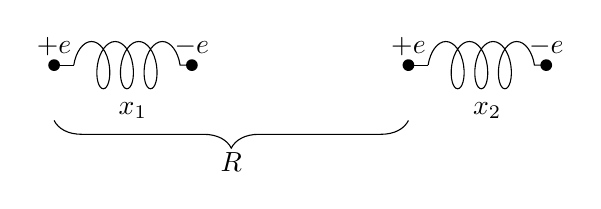
\begin{tikzpicture}
\draw[decoration={aspect=0.5, segment length=3mm, amplitude=3mm,coil},decorate] (0,0) --++ (1.5,0) node[fill=black,inner sep=1.5pt, circle]{} node[above]{$-e$} node[pos=0.5, below,yshift=-1em]{$x_1$};
\draw[] (0,0) --++ (-0.25,0) node[fill=black,inner sep=1.5pt,circle]{} node[above]{$+e$};
\draw[decoration={aspect=0.5, segment length=3mm, amplitude=3mm,coil},decorate] (4.5,0) --++ (1.5,0) node[fill=black,inner sep=1.5pt, circle]{} node[above]{$-e$} node[pos=0.5, below,yshift=-1em]{$x_2$};
\draw[] (4.5,0) --++ (-0.25,0) node[fill=black,inner sep=1.5pt,circle]{} node[above]{$+e$};
\draw[decorate,decoration={brace,amplitude=10pt,mirror},yshift=-20pt] (-0.25,0) -- (4.25,0) node[midway,yshift=-15pt]{$R$};
\end{tikzpicture}
\caption{دو  قابل تقطیب  قریبی جوہر (سوال \حوالہ{سوال_غیر_مضطرب_ون_در_وال})۔}
\label{شکل_غیر_تابع_اضطراب_قابل_تقطیب}
\end{figure}


ان جوہروں کے بیچ کولمب باہم عمل درج ذیل ہوگا ۔
\begin{align}\label{مساوات_غیر_مضطرب_جوہر_باہم_عمل}
H' = \frac{1}{4 \pi \epsilon_0} \big ( \frac{e^2}{R} - \frac{e^2}{R + x_1} - \frac{e^2}{R - x_2} + \frac{e^2}{R + x_1 - x_2} \big )
\end{align}
\begin{enumerate}[a.]
\item
مساوات  \حوالہ{مساوات_غیر_مضطرب_جوہر_باہم_عمل}  کی تفصیل پیش کریں۔  فاصلہ \عددی{ R} سے \عددی{|x_1|} اور \عددی{|x_2|} کی قیمتوں کو بہت کم تصور کرتے ہوئے درج ذیل دکھائیں ۔
\begin{align}\label{مساوات_غیر_مضطرب_تخمینی_ہیملٹنی}
H' \cong - \frac{e^2 x_1 x_2}{2 \pi \epsilon_0 R^3}
\end{align}
\item
دکھائیں کے کل ہیملٹنی  (مساوات \حوالہ {مساوات_غیر_مضطرب_جوہر_کل_ہیملٹنی}جمع مساوات  \حوالہ{مساوات_غیر_مضطرب_تخمینی_ہیملٹنی})   دو  ہارمونی مرتعش ہیملٹنیوں: 
\begin{align}
H = \big [ \frac{1}{2m} p_+^2 + \frac{1}{2} \big ( k - \frac{e^2}{4 \pi \epsilon_0 R^3} \big ) x_+^2 \big ] + \big [ \frac{1}{2m} p_-^2 + \frac{1}{2} \big ( k + \frac{e^2}{4 \pi \epsilon_0 R^3} \big ) x_-^2 \big ]
\end{align}
میں زیر  تبدیلی متغیرات:
\begin{align} 
 p \pm =  \frac{1}{\sqrt{2}} (p_1 \pm p_2) \quad \text{\RL{اور نتیجتاً}}\quad x \pm \equiv \frac{1}{\sqrt{2}} (x_1 \pm x_2)
\end{align}
علیحدہ علیحدہ ہو گی۔
\item
ظاہر ہے کہ اس ہیملٹنی کی زمینی حال توانائی درج ذیل ہوگی ۔
\begin{align}
 \omega_{\pm} = \sqrt{\frac{k \mp (e^2 / 4 \pi \epsilon_0 R^3)}{m}}\quad \text{\RL{جہاں}}\quad E = \frac{1}{2} \hslash (\omega_+ + \omega_- )
\end{align}
کولمب  باہم عمل کے بغیر یہ \عددی{E_0 = \hslash \omega_0 } ہوتی، جہاں \عددی{\omega_0 = \sqrt{k /m}} ہے۔
  یہ فرض کرتے ہوئے کہ  \عددی{k \gg (e^2 / 4 \pi \epsilon_0 R^3)} ہے، درج ذیل   دکھائیں۔ 
\begin{align}
\Delta V \equiv E - E_0 \cong - \frac{\hslash}{8m^2 \omega_0^3} \big ( \frac{e^2}{4 \pi \epsilon_0} \big )^2 \frac{1}{R^6}
\end{align}
\ترچھا{ماخوذ:} دو جوہروں کے بیچ  کششی  مخفیہ پایا جاتا ہے،   جو ان کے بیچ فاصلہ کے چھٹی  طاقت کے تغیر معکوس ہے۔ یہ دو معادل جوہروں کے بیچ \اصطلاح{ ون  در  و الس باہم عمل}\حاشیہب{Van der Waals interaction}\فرہنگ{Van der Waals interaction} ہے۔ 
\item
یہی  حساب  دو رتبی نظریہ اضطراب استعمال کرتے ہوئے  دوبارہ کریں۔ \ترچھا{ اشارہ:} غیر مضطرب حالات کا روپ \عددی{\psi_{n1} (x_1) \psi_{n2} (x_2)} ہوگا،  جہاں \عددی{\psi_n(x)} یک ذروی  مرتعش تفاعل موج ہے جس میں کمیت  \عددی{ m} اور مقیاس لچک \عددی{k} ہوگا؛ مساوات \حوالہ{مساوات_غیر_مضطرب_تخمینی_ہیملٹنی}  میں دی گئی اضطراب کے لیے زمینی حال توانائی کی دو رتبی تصحیح \عددی{\Delta V} ہوگی ( دھیان رہے کہ  اول رتبی  تصحیح صفر ہے)۔ 
\end{enumerate}
\انتہا{سوال}
\ابتدا{سوال}\شناخت{سوال_غیر_مضطرب_مسئلہ_فائنمن}
فرض کریں،  ایک مخصوص کوانٹائی نظام کی  ہیملٹنی  \عددی{H}،  کسی مقدار معلوم   \عددی{\lambda}  کی  تفاعل ہے؛\عددی{H(\lambda)} کی  امتیازی اقدار کو \عددی{E_{n}(\lambda)}،   اور امتیازی تفاعلات کو  \عددی{\psi_{n}(\lambda)} لیں۔   \اصطلاح{مسئلہ فائنمن و ہلمن}\فرہنگ{مسئلہ فائنمن و ہلمن}\حاشیہب{Feynmann-Hellmann theorem}\فرہنگ{Feynmann-Hellmann theorem}   درج ذیل کہتا ہے\حاشیہد{فائنمن نے مساوات \حوالہ{مساوات_غیر_مضطرب_مسئلہ_فائنمن} اپنی اعلٰی تعلیم کے دوران اخذ کی، جبکہ ہلمن   اسی مسئلہ کو چار سال قبل ایک غیر مشہور روسی   جریدہ میں کر چکے تھے۔}
\begin{align}\label{مساوات_غیر_مضطرب_مسئلہ_فائنمن}
\frac{\partial E_{n}}{\partial \lambda}=\big\langle{\psi_{n}|\frac{\partial{H}}{\partial{\lambda}}|\psi_{n}}\big\rangle
\end{align}
(جہاں  \عددی{E_{n}} کو غیر انحطاطی تصور کریں،  یا؛ اگر انحطاطی ہو تب،  تمام \عددی{\psi_{n}}کو انحطاطی امتیازی تفاعلات کے "موزوں" خطی جوڑ تصور کریں)۔
\begin{enumerate}[a.]
\item
   مسئلہ فائنمن و ہلمن    ثابت کریں۔\ترچھا{اشارہ :}   مساوات \حوالہ{مساوات_غیر_اضطراب_اہم_ترین} استعمال کریں ۔ 
\item
  اس کا اطلاق یک بُعدی  ہارمونی  مرتعش   پر  درج ذیل   صورتوں میں کریں۔
\begin{enumerate}[1.]  
\item
  \عددی{\lambda=\omega}لیں ( جو \عددی{V} کی توقعاتی قیمت کا کلیہ دیگا)، 
  \item
  \عددی{\lambda=\hslash}لیں (جو\عددی{\langle T \rangle}دے گا )، اور
  \item
  \عددی{\lambda=m}لیں (جو \عددی{\langle T \rangle}اور \عددی{\langle V \rangle}کا  رشتہ دے گا)۔
 \end{enumerate}
    اپنے جوابات کا سوال\حوالہ{سوال_شروڈنگر_تصدیق_کریں} اور مسئلہ  وریل   کی پیشنگوئیوں  (سوال \حوالہ{سوال_قواعد_مسئلہ_وریل})   کے ساتھ موازنہ  کریں ۔
 \end{enumerate}
\انتہا{سوال}
\ابتدا{سوال}\شناخت{سوال_غیر_مضطرب_مسئلہ_فائن_من} 
مسئلہ فائنمن و ہلمن (سوال \حوالہ{سوال_غیر_مضطرب_مسئلہ_فائنمن})  استعمال کرتے ہوئے ہائیڈروجن کے  لئے  \عددی{1/r} اور  \عددی{1/r^{2}} کی توقعاتی قیمتیں تعین  کی جا سکتی ہیں۔  رداسی تفاعلات موج    (مساوات \حوالہ{مساوات_ابعادی_رداسی_کولمب}) کی  موثر  ہیملٹنی  درج ذیل ہے 
\begin{align*}
H=-\frac{\hslash^{2}}{2m}\frac{\dif^{\,2}}{\dif r^{2}}+\frac{\hslash^{2}}{2m}\frac{l(l+1)}{r^{2}}-\frac{e^{2}}{4\pi\epsilon_0}\frac{1}{r}
\end{align*}
اور امتیازی اقدار  (جنہیں  \عددی{l} کی صورت میں لکھا گیا ہے)\حاشیہد{جزو-ب میں  ہم \عددی{l} کو استمراری متغیر تصور کرتے ہیں؛ یوں مساوات \حوالہ{مساوات_ابعادی_صدر_کوانٹائی_عدد}، جس میں \عددی{j_{\text{بلندتر}}} جو لازماً عدد صحیح ہو گا ایک مستقل ہے، کے تحت \عددی{n}متغیر \عددی{l} کا تفاعل ہو گا۔ ابہام دور کرنے کی غرض سے میں نے \عددی{n} کو خارج کیا تا کہ \عددی{l} پر  تابعیت  واضح ہو۔}  درج ذیل ہیں (  مساوات \حوالہ{مساوات_ابعادی_ہائیڈروجن_اجازتی_توانائیاں} )۔
\begin{align*}
E_n=-\frac{me^{4}}{32\pi^{2}\epsilon_0^{2}\hslash^{2}(j_{\text{\RL{بلندتر}}}+l+1)^{2}}
\end{align*}
\begin{enumerate}[a.]
\item
 مسئلہ  فائنمن و ہلمن  میں   \عددی{\lambda=e} لیتے  ہوئے \عددی{\langle1/r\rangle} تلاش کریں۔ اپنے نتیجے کی تصدیق مساوات  \حوالہ{مساوات_غیر_مضطرب_آر_ایک}  سے  کریں۔
\item
\عددی{\lambda=l} لیتے  ہوئے \عددی{\langle1/r^{2}\rangle} تلاش کریں۔ اپنے نتیجے کی تصدیق مساوات  \حوالہ{مساوات_غیر_مضطرب_آر_دوم}  سے  کریں۔
\end{enumerate}
\انتہا{سوال}
\ابتدا{سوال}
 \اصطلاح{رشتہ  کرامرس}:\فرہنگ{رشتہ!کرامرس}\حاشیہب{Kramers' relation}\فرہنگ{relation!Kramers} 
\begin{align}\label{مساوات_غیر_مضطرب_رشتہ_کرامرس}
\frac{s+1}{n^{2}}\langle r^{s}\rangle -(2s+1)a\langle r^{s-1}\rangle +\frac{s}{4}[(2l+1)^{2}-s^{2}]a^{2}\langle r^{s-2}\rangle =0
\end{align}
ثابت  کریں؛\حاشیہد{اس تعلق کو  \اصطلاح{رشتہ پسترنک}\فرہنگ{رشتہ!پسترنک}\فرہنگ{relation!Pasternack} بھی کہتے ہیں۔}    یہ   ہائیڈروجن کے حال  \عددی{\psi_{nlm}} میں الیکٹران کے لئے،  \عددی{r}کی    تین مختلف طاقتوں  (\عددی{s}، \عددی{s-1} اور \عددی{s+1})  کے     توقعاتی قیمتوں کا    تعلق پیش کرتا ہے۔  \ترچھا{اشارہ :}  رداسی مساوات  (مساوات \حوالہ{مساوات_ابعادی_رداسی_کولمب})  کو درج ذیل روپ میں لکھ کر
\begin{align*}
u''=\big[\frac{l(l+1)}{r^{2}}-\frac{2}{ar}+\frac{1}{n^{2}a^{2}}\big]u
\end{align*}
\عددی{\int(ur^{s}u'')\dif r} کو   \عددی{\langle r^{s}\rangle}، \عددی{\langle r^{s-1}\rangle}، \عددی{\langle r^{s-2}\rangle } کی  صورت میں لکھیں۔  اس کے بعد تکمل بالحصص  کے ذریعہ دہرے  تفرق  کو  گھٹائیں۔ دکھائیں کہ 
\begin{align*}
\int(ur^{s}u')\dif r&=-(s/2)<r^{s-1}>\\
\int(u'r^{s}u')\dif r&=-[2/(s+1)]\int(u''r^{s+1}u')\dif r&&\text{اور}
\end{align*}
ہوں گے۔یہاں سے آگے چلیں۔
\انتہا{سوال}
\ابتدا{سوال} \شناخت{سوال_غیر_مضطرب_طاقتی_توقعاتی_قیمتیں}
\begin{enumerate}[a.]
\item
 رشتہ  کرامرس   (مساوات  \حوالہ{مساوات_غیر_مضطرب_رشتہ_کرامرس})   میں \عددی{s=0}، \عددی{s=1}، \عددی{s=2}  اور  \عددی{s=3} ڈال کر   
\عددی{\langle r^{-1}\rangle}، \عددی{\langle r\rangle}، \عددی{\langle r^{2}\rangle}،  اور \عددی{\langle r^{3}\rangle}
 کے کلیات حاصل کریں۔ آپ دیکھ سکتے ہیں کہ  اس طرح چلتے ہے کسی بھی مثبت طاقت کے  کلیات  دریافت کیے جا سکتے  ہیں ۔
\item
البتہ، \ترچھا{مخالف}   رخ چلتے ہوئے  آپ کو ایک  مسئلہ  درپیش  ہوگا۔  آپ  \عددی{s=-1} ڈال  کر دیکھ سکتے ہیں  کہ صرف  \عددی{\langle r^{-2}\rangle} اور 
  \عددی{\langle r^{-3}\rangle} کا  رشتہ حاصل ہو  تا ہے۔
\item
 اگر آپ کسی دوسرے طریقے سے  \عددی{\langle r^{-2}\rangle}  دریافت کر پائیں،  تب آپ رشتہ کرامرس  استعمال کرکے باقی تمام منفی قوتوں کے لئے کلیات دریافت کر سکتے ہیں ۔
مساوات  \حوالہ{مساوات_غیر_مضطرب_آر_دوم} (  جو سوال \حوالہ{سوال_غیر_مضطرب_مسئلہ_فائن_من} میں اخذ کی گئی ہے)    استعمال کرتے ہوئے  \عددی{\langle r^{-3}\rangle}
تعین کریں،  اور اپنے نتیجہ کی تصدیق مساوات \حوالہ{مساوات_غیر_مضطرب_آر_تین} کے ساتھ کریں۔
\end{enumerate}
\انتہا{سوال}
\ابتدا{سوال}\شناخت{سوال_غیر_مضطرب_شٹارک_اثر}
 جوہر کو    یکساں   بیرونی برقی میدان \عددی{E_{\text{بیرونی}}} میں رکھنے سے اس کی  سطحیں   توانائی  اپنی جگہ سے سرک جاتی  ہیں،  جسے \اصطلاح{ شٹارک  اثر}\فرہنگ{شٹارک اثر}\حاشیہب{Stark effect}\فرہنگ{Stark effect}  کہتے ہیں ( اور جو  زیمان  اثر کا برقی مماثل ہے)۔ اس سوال میں ہم ہائیڈروجن کے  \عددی{n=1} اور  \عددی{n=2} حالات کے لئے شٹارک اثر کا تجزیہ کرتے ہیں۔ فرض کریں میدان \عددی{z} رخ ہے،  لہٰذا الیکٹران کی مخفی توانائی درج ذیل ہوگی۔
\begin{align*}
H'_{S}=eE_{\text{بیرونی}}z=eE_{\text{بیرونی}}r\cos{\theta}
\end{align*}
اس کو بوہر ہیملٹنی  (مساوات\حوالہ{مساوات_غیر_مضطرب_بوہر_ہیملٹنی}) میں اضطراب تصور کریں۔ ( اس مسئلہ میں چکر کا کوئی کردار نہیں ہے،  لہٰذا اسے نظر انداز کریں،  اور   مہین  ساخت کو  نظرانداز  کریں۔)
\begin{enumerate}[a.]
\item
 دکھائیں کہ اول رتبہ میں زمینی حال توانائی اس اضطراب سے اثر انداز نہیں ہوتی ۔
\item
پہلا ہیجان حال \عددی{4} پڑتا انحطاطی:    \عددی{\psi_{200}}، \عددی{\psi_{211}}، \عددی{\psi_{210}}، \عددی{\psi_{21-1}}  ہے۔ انحطاطی نظریہ اضطراب استعمال کرتے ہوئے، توانائی کی   اول رتبی  تصحیح  تعین کریں ۔توانائی  \عددی{E_{2}} کا بٹوارا  کتنے سطحوں میں  ہو گا؟
\item
 درج بالا جزو-ب میں "موزوں" تفاعلات موج کیا ہونگے ؟  ہر ایک "موزوں" حال میں برقی جفت  قطب معیار اثر \عددی{(\kvec{p}_e=-e\kvec{r})} کی توقعاتی قیمت معلوم کریں ۔ آپ دیکھیں گے کہ نتائج  لاگو کیے گئے  میدان کے تابع نہیں ہیں؛   ظاہر ہے کہ  پہلے  ہیجان حال میں ہائیڈروجن ایک \ترچھا{ دائمی}  برقی جفت قطب معیار اثر کا حامل ہوگا۔
 
  \ترچھا{اشارہ:} اس سوال میں بہت سارے تکملات  پائے جاتے ہیں،  تاہم  تقریباً  تمام کی قیمت صفر  ہے۔  اس لئے  حساب سے قبل غور کریں،  اگر  \عددی{\phi} تکمل  صفر ہو تو   \عددی{r} اور  \عددی{\theta} تکملات حل کرنے  کی ضرورت نہیں ہوگی۔اگر \عددی{\phi} تکمل صفر ہو، \عددی{r} اور \عددی{\theta} تکملات کا حساب کرنا بے معنی ہو گا! \ترچھا{   جزوی جواب:} \عددی{W_{13}=W_{31}=-3eaE_{\text{بیرونی}}}؛ باقی تمام ارکان صفر ہیں۔ 
\end{enumerate}
\انتہا{سوال}
%KKK 23 jan 2022 edited till here
\ابتدا{سوال}
 ہائیڈروجن کے \عددی{n=3} حالات کے لئے شٹارک  اثر (سوال \حوالہ{سوال_غیر_مضطرب_شٹارک_اثر})پر غور کرتے ہیں۔  ابتدائی  طور پر  (پہلے کی طرح، چکر کو نظر انداز کرتے ہوئے)  نو  انحطاطی حالات 
\عددی{\psi_{3lm}} ہونگے،  اور اب ہم  \عددی{z} رخ برقی میدان چالو کرتے ہیں۔
\begin{enumerate}[a.]
\item
اضطرابی  ہیملٹنی  کو ظاہر کرنے والا  \عددی{9\times9} قالب   تیار کریں۔ \ترچھا{ جزوی جواب:}
\begin{align*}
\langle 300|z|310\rangle =-3\sqrt{6}\,a,\,\,\langle 310|z|320\rangle =-3\sqrt{3}\,a,\,\,\langle 31\pm1|z|32\pm1\rangle=-(9/2)a
\end{align*}
\item 
امتیازی اقدار اور انکے انحطاط  دریافت کریں۔ 
\end{enumerate}
\انتہا{سوال}
\ابتدا{سوال}
\اصطلاح{  ڈیوٹریم}\فرہنگ{ڈیوٹریم}\حاشیہب{deuterium}\فرہنگ{deuterium} کے  زمینی حال \عددی{(n=1)} میں نہایت مہین منتقلی کی بدولت   خارج  نوریہ  کا طول موج ، سنٹی میٹروں میں،  تلاش کریں ۔ ڈیوٹریم درحقیقت "بھاری"  ہائیڈروجن ہے ، جس کے مرکز میں ایک اضافی نیوٹران پایا جاتا ہے؛ پروٹان اور نیوٹران  کی بندش سے  \اصطلاح{ڈیوٹیران}\فرہنگ{ڈیوٹیران}\حاشیہب{deuteron}\فرہنگ{deuteron}   پیدا ہوتا ہے،  جس کا چکر \عددی{1} اور  مقناطیسی معیار اثر
\begin{align*}
\kvec{\mu}_{d}=\frac{g_{d}e}{2m_{d}}\kvec{S}_{d}
\end{align*}
ہے؛   ڈیوٹریم کا \عددی{g}  جزو ضربی \عددی{ 1.71} ہے ۔
\انتہا{سوال}
\ابتدا{سوال}\شناخت{سوال_غیر_مضطرب_قلم}
 ایک قلم میں قریبی  بارداریہ  کے برقی میدان جوہر کی سطحیں   توانائی   کو مضطرب کرتے ہیں۔ سادہ نمونہ کے طور پر   (شکل \حوالہ{شکل_غیر_تابع_اضطراب_قلمی_جال})،    فرض کریں  ہائیڈروجن  جوہر کے گرد  نقاطی  بار  کی تین جوڑیاں پائی جاتی ہیں ۔(چونکہ    چکر  اس سوال سے   غیر متعلقہ  ہے،  لہٰذا اسے نظرانداز کریں۔ )
 
 \begin{figure}
\centering
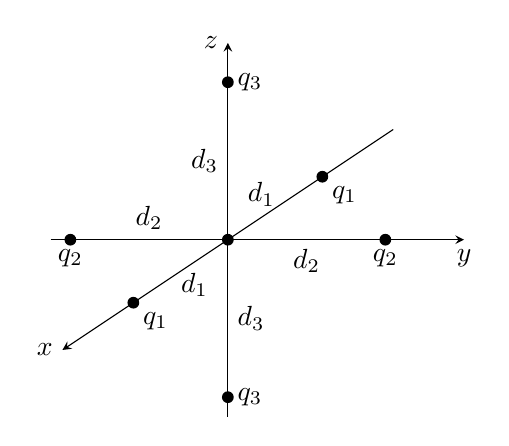
\begin{tikzpicture}[x={(-0.6cm,-0.4cm)},y={(1cm,0cm)},z={(0cm,1cm)}]
\draw[-stealth](0,-2.25,0) -- (0,3,0) node[below]{$y$};
\draw[-stealth](-3.5,0,0) -- (3.5,0,0) node[left]{$x$};
\draw[-stealth](0,0,-2.25) -- (0,0,2.5) node[left]{$z$};
\draw[](-2,0,0) node[fill=black,inner sep=1.5pt,circle]{} node[below right]{$q_1$};
\draw[](2,0,0) node[fill=black,inner sep=1.5pt,circle]{} node[below right]{$q_1$};
\draw[](0,-2,0) node[fill=black,inner sep=1.5pt,circle]{} node[below]{$q_2$};
\draw[](0,2,0) node[fill=black,inner sep=1.5pt,circle]{} node[below]{$q_2$};
\draw[](0,0,-2) node[fill=black,inner sep=1.5pt,circle]{} node[right]{$q_3$};
\draw[](0,0,2) node[fill=black,inner sep=1.5pt,circle]{} node[right]{$q_3$};
\draw[] (-1,0,0) node[shift={(-5pt,5pt)}]{$d_1$};
\draw[] (1,0,0) node[shift={(5pt,-5pt)}]{$d_1$};
\draw[] (0,-1,0) node[above]{$d_2$};
\draw[] (0,1,0) node[below]{$d_2$};
\draw[] (0,0,-1) node[right]{$d_3$};
\draw[] (0,0,1) node[left]{$d_3$};
\draw(0,0,0) node[circle,fill=black,inner sep=1.5pt]{};
\end{tikzpicture}
\caption{ہائیڈروجن جوہر کے گرد   چھ نقطی بار (قلمی جال کا ایک سادہ نمونہ؛سوال \حوالہ{سوال_غیر_مضطرب_قلم})۔ }
\label{شکل_غیر_تابع_اضطراب_قلمی_جال}
\end{figure}
%
\begin{enumerate}[a.]
\item
   فرض کریں \عددی{r\ll d_{1}}،   \عددی{r\ll d_{2}}، اور    \عددی{r\ll d_{3}} ہے۔ دکھائیں   :
\begin{align*}
H'=V_{o}+3(\beta_{1}x^{2}+\beta_{2}y^{2}+\beta_{3}z^{2})-(\beta_{1}+\beta_{2}+\beta_{3})r^{2},
\end{align*}
 جہاں  درج ذیل ہیں۔
\begin{align*}
\beta_{i}\equiv-\frac{e}{4\pi\epsilon_0}\frac{q_{i}}{d_{i}^{3}},\quad\quad V_{o}=2(\beta_{1}d_{1}^{2}+\beta_{2}d_{2}^{2}+\beta_{3}d_{3}^{2})
\end{align*}
\item
زمینی حال توانائی کی  اول  رتبی  تصحیح تلاش کریں ۔
\item
 پہلے  ہیجان حالات  \عددی{(n=2)}  کی توانائی کے    اول  رتبی  تصحیح تلاش کریں ۔ درج ذیل صورتوں میں اس  چار پڑتا  انحطاطی نظام کا بٹوارا  کتنے سطحوں میں  ہو  گا؟
 \begin{enumerate}[1.]
\item
 \اصطلاح{کعبی  تشاکل}\فرہنگ{کعبی تشاکل}\حاشیہب{cubic symmetry}\فرہنگ{cubic symmetry}،  \عددی{\beta_{1}=\beta_{2}=\beta_{3}}؛
\item
 \اصطلاح{چو  زاویہ تشاکل}\فرہنگ{چو زاویہ تشاکل}\حاشیہب{tetragonal symmetry}\فرہنگ{tetragonal symmetry}،
  \عددی{\beta_{1}=\beta_{2}\neq\beta_{3}}؛
\item
 \اصطلاح{قائمی معّین}\فرہنگ{قائمی معّین}\حاشیہب{orthorhombic symmetry}\فرہنگ{orthorhombic symmetry}  تشاکل کی  عمومی   صورت (جس میں تینوں مختلف ہوں گے) ۔
\end{enumerate}
\end{enumerate}
\انتہا{سوال}
\ابتدا{سوال}
بعض اوقات   \عددی{\psi_{n}^{1}} کو غیر مضطرب تفاعلات موج (  مساوات \حوالہ{مساوات_غیر_اضطراب_تصحیح_اول_تفاعل}) میں پھیلائے   بغیر مساوات  \حوالہ{مساوات_غیر_اضطراب_تصحیح_اول_توانائی} کو بلا واسطہ حال کرنا ممکن ہوتا ہے۔  اسکی دو   خوبصورت مثالیں  درج ذیل ہیں۔
\begin{enumerate}[a.]
\item
 \موٹا{ہائیڈروجن کے زمینی حال میں شٹارک اثر۔} 
 \begin{enumerate}[1.]
 \item
  یکساں بیرونی برقی میدان  \عددی{E_{\text{بیرونی}}} کی صورت  میں ہائیڈروجن  کے  زمینی حال کا   اول رتبی  تصحیح  تلاش کریں ( سوال   \حوالہ{سوال_غیر_مضطرب_شٹارک_اثر} ؛ شٹارک  اثر دیکھیں ) ۔\ترچھا{اشارہ :} حل کا  درج ذیل روپ 
\begin{align*}
(A+Br+Cr^{2})e^{-r/a}\cos\theta
\end{align*}
استعمال کرکے دیکھیں؛  آپ نے مستقلات  \عددی{A} \عددی{B}،  اور  \عددی{C} کی ایسی قیمتیں تلاش کرنی ہیں جو مساوات  \حوالہ{مساوات_غیر_اضطراب_تصحیح_اول_توانائی} کو مطمئن کرتی  ہوں ۔
\item
 زمینی حال توانائی کی  دوم  رتبی تصحیح   مساوات  \حوالہ{مساوات_غیر_مضطرب_دوم_رتبی_تصحیح}  کی مدد سے  تعین کریں ( جیسا اپنے سوال  \حوالہ{سوال_غیر_مضطرب_شٹارک_اثر}-الف  میں دیکھا    اول  رتبی تصحیح  صفر ہوگی) ۔\ترچھا{جواب:} \عددی{-m(3a^{2}eE_{\text{بیرونی}}/2\hslash)^{2}}
\end{enumerate}
\item
 اگر پروٹان کا \ترچھا{برقی}  جفت قطب  معیار اثر  \عددی{p} ہوتا،  تو  ہائیڈروجن میں  الیکٹران  کی مخفی توانائی درج ذیل مقدار سے مضطرب ہوتی۔
\begin{align*}
H'=\frac{ep\cos\theta}{4\pi\epsilon _0r^{2}}
\end{align*}
\begin{enumerate}[1.]
\item
 زمینی حال تفاعل موج کی  اول  رتبی تصحیح  کو مساوات  \حوالہ{مساوات_غیر_اضطراب_تصحیح_اول_توانائی} حل کرکے تلاش کریں ۔
\item
 دکھائیں  کہ  اس رتبہ تک جوہر کا  \ترچھا{کل}  برقی جفت قطب معیار اثر( حیرت کی بات ہے)  صفر ہے۔ 
\item
 زمینی حال توانائی کی   دوم  رتبی تصحیح  مساوات \حوالہ{مساوات_غیر_مضطرب_دوم_رتبی_تصحیح}  سے تعین کریں۔  اول رتبی  تصحیح  کتنی  ہوگی ؟
\end{enumerate}
\end{enumerate}
\انتہا{سوال}

